% Copyright (c) 2008-2009 solvethis
% Copyright (c) 2010-2016 Casper Ti. Vector
% Public domain.
%
% 使用前请先仔细阅读 pkuthss 和 biblatex-caspervector 的文档,
% 特别是其中的 FAQ 部分和用红色强调的部分。
% 两者可在终端/命令提示符中用
%   texdoc pkuthss
%   texdoc biblatex-caspervector
% 调出。

% 采用了自定义的(包括大小写不同于原文件的)字体文件名,
% 并改动 ctex.cfg 等配置文件的用户请自行加入 nofonts 选项;
% 其它用户不用加入 nofonts 选项,加入之后反而会产生错误。
\documentclass[UTF8]{pkuthss}

% 使用 biblatex 排版参考文献,并规定其格式(详见 biblatex-caspervector 的文档)。
% 这里按照英文文献在前,中文文献在后排序(“sorting = ecnty”);
% 若需按照中文文献在前,英文文献在后排序,请设置“sorting = centy”;
% 若需按照引用顺序排序,请设置“sorting = none”。
% 若需在排序中实现更复杂的需求,请参考 biblatex-caspervector 的文档。
\usepackage[backend = biber, style = caspervector, utf8, sorting = ecnty]{biblatex}

\usepackage{amsmath}
\usepackage{algorithm}
\usepackage{algorithmic}
\usepackage{url}
\usepackage{tabularx}
\usepackage{subcaption}

% \usepackage[demo]{graphicx}
% \usepackage{caption}
% \usepackage{subfig}


% 按学校要求设定参考文献列表中的条目之内及之间的距离。
\setlength{\bibitemsep}{3bp}
% 对于 linespread 值的计算过程有兴趣的同学可以参考 pkuthss.cls。
\renewcommand*{\bibfont}{\zihao{5}\linespread{1.27}\selectfont}

% 设定文档的基本信息。
\pkuthssinfo{
	cthesisname = {硕士研究生学位论文}, ethesisname = {Master Thesis},
	ctitle = {基于部分共享的高速缓存分配优化}, etitle = {Cache Allocation with Partial Sharing},
	cauthor = {黄子翚},
	eauthor = {Huang Zihui},
	studentid = {1401214258},
	date = {二〇一七年六月},
	school = {信息科学技术学院},
	cmajor = {计算机软件与理论}, emajor = {Computer Science},
	direction = {系统虚拟化技术},
	cmentor = {罗英伟教授}, ementor = {Prof.\ Luo Yingwei},
	ckeywords = {高速缓存,多核,分配优化,部分共享}, ekeywords = {CAT, Multicore, Optimization, Partial-sharing}
}
% 载入参考文献数据库(注意不要省略“.bib”)。
\addbibresource{thesis.bib}

% 普通用户可删除此段,并相应地删除 chap/*.tex 中的
% “\pkuthssffaq % 中文测试文字。”一行。
\usepackage{color}
\def\pkuthssffaq{%
	\emph{\textcolor{red}{pkuthss 文档模版最常见问题:}}

	\texttt{\string\cite}、\texttt{\string\parencite} %
	和 \texttt{\string\supercite} 三个命令分别产生%
	未格式化的、带方括号的和上标且带方括号的引用标记:%
	\cite{test-en},\parencite{test-zh}、\supercite{test-en, test-zh}。

	若要避免章末空白页,请在调用 pkuthss 文档类时加入 \texttt{openany} 选项。

	如果编译时不出参考文献,
	请参考 \texttt{texdoc pkuthss}“问题及其解决”一章
	“其它可能存在的问题”一节中关于 biber 的说明。
}

\begin{document}
	% 以下为正文之前的部分,默认不进行章节编号。
	\frontmatter
	% 此后到下一 \pagestyle 命令之前不排版页眉或页脚。
	\pagestyle{empty}
	% 自动生成封面。
	\maketitle
	% 版权声明。封面要求单面打印,故需新开右页。
	\cleardoublepage
	% Copyright (c) 2008-2009 solvethis
% Copyright (c) 2010-2017 Casper Ti. Vector
% All rights reserved.
%
% Redistribution and use in source and binary forms, with or without
% modification, are permitted provided that the following conditions are
% met:
%
% * Redistributions of source code must retain the above copyright notice,
%   this list of conditions and the following disclaimer.
% * Redistributions in binary form must reproduce the above copyright
%   notice, this list of conditions and the following disclaimer in the
%   documentation and/or other materials provided with the distribution.
% * Neither the name of Peking University nor the names of its contributors
%   may be used to endorse or promote products derived from this software
%   without specific prior written permission.
%
% THIS SOFTWARE IS PROVIDED BY THE COPYRIGHT HOLDERS AND CONTRIBUTORS "AS
% IS" AND ANY EXPRESS OR IMPLIED WARRANTIES, INCLUDING, BUT NOT LIMITED TO,
% THE IMPLIED WARRANTIES OF MERCHANTABILITY AND FITNESS FOR A PARTICULAR
% PURPOSE ARE DISCLAIMED. IN NO EVENT SHALL THE COPYRIGHT HOLDER OR
% CONTRIBUTORS BE LIABLE FOR ANY DIRECT, INDIRECT, INCIDENTAL, SPECIAL,
% EXEMPLARY, OR CONSEQUENTIAL DAMAGES (INCLUDING, BUT NOT LIMITED TO,
% PROCUREMENT OF SUBSTITUTE GOODS OR SERVICES; LOSS OF USE, DATA, OR
% PROFITS; OR BUSINESS INTERRUPTION) HOWEVER CAUSED AND ON ANY THEORY OF
% LIABILITY, WHETHER IN CONTRACT, STRICT LIABILITY, OR TORT (INCLUDING
% NEGLIGENCE OR OTHERWISE) ARISING IN ANY WAY OUT OF THE USE OF THIS
% SOFTWARE, EVEN IF ADVISED OF THE POSSIBILITY OF SUCH DAMAGE.

% 此处不用 \specialchap,因为学校要求目录不包括其自己及其之前的内容。
\chapter*{版权声明}
% 综合学校的书面要求及 Word 模版来看,版权声明页不需加页眉、页脚。
\thispagestyle{empty}

任何收存和保管本论文各种版本的单位和个人,
未经本论文作者同意,不得将本论文转借他人,
亦不得随意复制、抄录、拍照或以任何方式传播。
否则一旦引起有碍作者著作权之问题,将可能承担法律责任。

% 若需排版二维码,请将二维码图片重命名为“barcode”,
% 转为合适的图片格式,并放在当前目录下,然后去掉下面 2 行的注释。
%\vfill\noindent
%\includegraphics[height = 5em]{barcode}

% vim:ts=4:sw=4


	% 此后到下一 \pagestyle 命令之前正常排版页眉和页脚。
	\cleardoublepage
	\pagestyle{plain}
	% 重置页码计数器,用大写罗马数字排版此部分页码。
	\setcounter{page}{0}
	\pagenumbering{Roman}
	% 中英文摘要。
	% Copyright (c) 2014,2016 Casper Ti. Vector
% Public domain.

\begin{cabstract}
随着处理器多核技术的广泛应用,多个程序可以在不同的核上并发执行。然而,并发执行的程序会在底层共享缓存(LLC)层面产生竞争,从而出现严重的性能下降。如何有效地对共享缓存进行调控和优化是被学术界广泛研究的一个问题。现有的解决方案大多数依赖硬件层面对缓存进行划分,从而满足性能或服务质量(QoS)等方面的要求。但是,这些硬件方案都只能在模拟器中进行模拟,并没有在真实系统中实现。直到最近英特尔在服务器级处理器中引入了高速缓存分配技术(CAT)。高速缓存分配技术基于缓存的路(Cache Way),所以只能在粗粒度上进行缓存分配。直接使用高速缓存分配技术进行不重叠的划分,在并发运行的线程数较多时,并不能很好的满足各种各样的优化目标。为了克服这些限制,我们刻意地将部分划分进行重叠,通过精确的重叠控制来提升分配的粒度。

本文提出了一个支持部分共享的高速缓存分配优化框架(CAPS)。它可以在较细的粒度上实现对缓存占用的控制。CAPS基于英特尔高速缓存分配技术,并且可以在真实系统中运行,它主要包含预测和分配两个模块。预测模块负责在任意重叠的缓存分配情况下对每个并发执行程序的缓存失效率和周期指令数进行预测,分配模块负责在给定一个优化目标后生成一个优化分配策略。CAPS可以支持多种优化目标,并且在并发程序数较大时也有很好的兼容性。在本文中我们实现了五种优化策略:失效数最小化,吞吐量最大化,以及三种性能下降指标的最小化。我们对75组并发工作负载进行实验评估,每组负载包括4到15个SPEC CPU2006测试程序。平均来看,相比于自由竞争使用LLC,CAPS可以降低16.96\%的失效数,提升11.11\%的吞吐量,减少8.16\%的平均性能损失,在兼顾公平和性能的指标上提升8.17\%,将性能下降最严重的程序提升23.24\%。
\end{cabstract}


\begin{eabstract}
In a multicore system, simultaneously executed programs may suffer from performance degradation due to contention on the shared last level cache (LLC). Effective management of LLC has attracted significant research attention. Existing solutions often rely on hardware cache partitioning to ensure performance and quality of service. However, none of these hardware partitioning schemes had been implemented on a real system until Intel introduced Cache Allocation Technology (CAT) to its commodity processors recently. CAT itself implements way partitioning and thus can only allocate at a coarse granularity. It does not scale well for a large thread or program count to serve their various performance goals effectively. We overcome these limitations by deliberately and precisely sharing part of the allocations among programs and cores.

In this paper, we propose Cache Allocation with Partial Sharing (CAPS), a framework that manages shared cache occupancy at a fine granularity. It is implemented on top of CAT, and runs on the real system. CAPS consists of two parts: (1) a prediction model that estimates miss rates and IPCs of a multiprogrammed workload under any partially-overlapping CAT scheme, and (2) a simulated annealing algorithm that outputs a near-optimal solution given a specific performance goal. CAPS is able to support a wide range of performance targets and can scale to a large core count. We demonstrate its flexibility by implementing five policies targeting average MPKI, IPC throughput, average slowdown, fair slowdown and maximum slowdown, respectively. Our evaluation, with 75 workloads ranging from 4-program to 15-program co-run, shows that on average, CAPS can reduce average MPKI by 16.96\%, increase throughput by 11.11\%, cut average slowdown by 8.16\%, improve fair slowdown by 8.17\%, and lower maximum slowdown by 23.24\%, when compared to full-sharing.
\end{eabstract}

% vim:ts=4:sw=4

	% 自动生成目录。
	\tableofcontents

	% 以下为正文部分,默认要进行章节编号。
	\mainmatter
	% 序言。
	% Copyright (c) 2014,2016 Casper Ti. Vector
% Public domain.

\chapter{序言} \label{chap:introduction}
随着多处理器、多核技术的迅猛发展,多核处理器(CMP)中的核数也越来越多。核数增加一个显而易见的优点就是可以支持更多的程序并发执行,然而这也导致了存储访问的瓶颈变得尤为突出。由于中央处理器(CPU)的运算速度远远高于其访问内存的速度,为了缓解这个速度差异,通常在CPU与内存之间会设有多级高速缓存(Cache)。在多核处理器中,每个核会有1到2级私有缓存,同时所有核会共享一个底层缓存(LLC)。由于缓存大小有限,并发执行的程序会对这层共享缓存进行竞争,竞争的结果就是每个程序的性能都或多或少受到损失。

目前CPU大多采用基于LRU的缓存替换策略,它对所有的缓存访问,不管来源于哪个核,都“一视同仁”。这就带来了一个问题:一个污染性高的程序会占据大量的缓存空间,从而压缩了其他程序的缓存使用,导致它们的失效率升高,性能下降。长期以来,国内外对这个问题展开了大量的研究工作,但是并没有真正解决,尤其在真实系统环境下。前人的研究大多依赖于硬件/软件层面上对共享缓存进行划分,通过对缓存插入和替换策略的调优来改善系统效率。然而,它们都有一个共同的缺点:无法应用到真实系统上。

基于硬件的方法主要是在模拟器中进行实现~\parencite{suh2004dynamic,qureshi2006utility,qureshi2007adaptive,hsu2006communist,iyer2004cqos,kim2004fair,rafique2006architectural,xie2009pipp}。然而模拟器存在多方面的不足,比如运行速度较慢、准确度不够等等。通常一个基于模拟器的实验会运行几十亿条指令,这仅仅相当于实际运行的几秒钟。一个程序的结构和行为的复杂性无法在这么短的执行时间里体现出来。所以我们认为对于一个缓存优化方案,必须要经过长时间的执行才能证明其有效性。

基于软件的方法主要是通过页面着色技术(Page Coloring)。它通过操作系统对页面映射进行控制,从而完成对缓存占用的控制。页面着色技术本可以应用在真实系统中,然而现代处理器纷纷改用哈希算法,而不是原先一一对应的方式,来进行内存地址到缓存块的映射。所以页面着色技术目前也不再适用。

缓存调控的另一个关键点是分配的粒度。粗粒度分配技术一般是基于缓存路的划分(Way Partitioning)~\parencite{suh2004dynamic,qureshi2006utility,qureshi2007adaptive,hsu2006communist,iyer2004cqos,kim2004fair,rafique2006architectural,xie2009pipp}。一个路往往含有多个缓存块(Block),划分的时候不能把一个路切开分给两个不同的线程,并且由于体系结构的限制,路的个数不能无限制增加。所以基于路的缓存划分涉及的硬件改动较小,但是粒度较粗。另外一些研究提出了细粒度划分技术~\parencite{sanchez2011vantage,manikantan2012probabilistic,chang2014cooperative}。虽然细粒度划分提供了更强的可扩展性和灵活性,但是需要更加复杂的设计和更多的硬件改动。考虑到设计的简洁性,大部分研究还是采用了粗粒度的路划分技术。正如前文所说,路划分下分配的最小单位是路的大小。在核数/线程数增加的情况下,它的效率就会下降,因为最优的划分很可能会切在一个路的中间。极端情况下当核数/线程数等于总路数,每个线程有且只能有一个路的缓存分配,这就彻底失去了分配的灵活性。一些研究试图在保留路分配的基础上,细化分配粒度。Probabilistic Shared-Cache Management(PriSM)通过精确控制驱逐(Eviction)概率来把粒度变得更细~\parencite{manikantan2012probabilistic}。Cooperative Cache Partitioning(CCP)通过时域共享,在不同的时间片用不同的分配方案,来细化分配粒度。不过,这些研究都需要或多或少的改动硬件,所以只是在模拟器中进行实验,而暂时无法应用到实际系统中。

在本文中,我们提出了CAPS(Cache Allocation with Partial Sharing),一个基于部分共享的缓存分配优化框架。CAPS在真实系统上实现了细粒度的缓存分配,是一个纯软件的框架。CAPS依赖于英特尔高速缓存分配技术(CAT)。CAT是英特尔最近才在服务器处理器中全线引入的功能,首次在商业处理器上实现了对高速缓存的管理。CAT也是基于路的划分,所以本身是一个粗粒度的分配技术。CAT技术中可分配的路数非常有限,在最高端的处理器上也只有20个路可供分配,每个路包含数个MB的缓存空间。为此,我们提出了通过空间共享的方式来细化分配粒度。分配间的部分重叠是被CAT所允许的。通过精确地控制分配以及之间的重叠,我们可以实现一个较细粒度的缓存管理。

我们用一个小例子来说明部分共享如何优于完全共享和不共享的分配。两个SPEC CPU2006的测试程序470.lbm和471.omnetpp分别运行在两个核上,它们共享一个4路高速缓存,每路含有2816KB的缓存资源。我们在真实机器上实验了所有可能的CAT分配方案,然后选择最优的重叠方案和不重叠方案。最优这里指的是IPC(周期指令数)吞吐量的最大化,也就是这两个程序的IPC之和最大。图 \ref{fig:illustration} (a) 展示了这三种方案的分配布局,从上到下分别是:传统的完全共享LLC(full share),最优的不重叠分配(non-overlapping),和最优的重叠分配(overlapping)。图 \ref{fig:illustration} (b) 比较了这三种方案的IPC吞吐量。不难看出,部分重叠的分配方案比另外两种方案都要更优。完全重叠下两个程序的平均IPC分别为0.347465和0.954963,不重叠下分别为0.421380和0.912704, 部分重叠下为0.415268和0.967625。部分重叠相比于完全重叠,两个程序的IPC都获得提升,而相比于不重叠分配,虽然470.lbm的IPC稍微损失了一点,但471.omnetpp得到了很大的提升,所以加总的IPC吞吐量也获得了提升。

\begin{figure}[htbp] 
    \centering
    \begin{subfigure}[b]{0.4\linewidth}
        \centering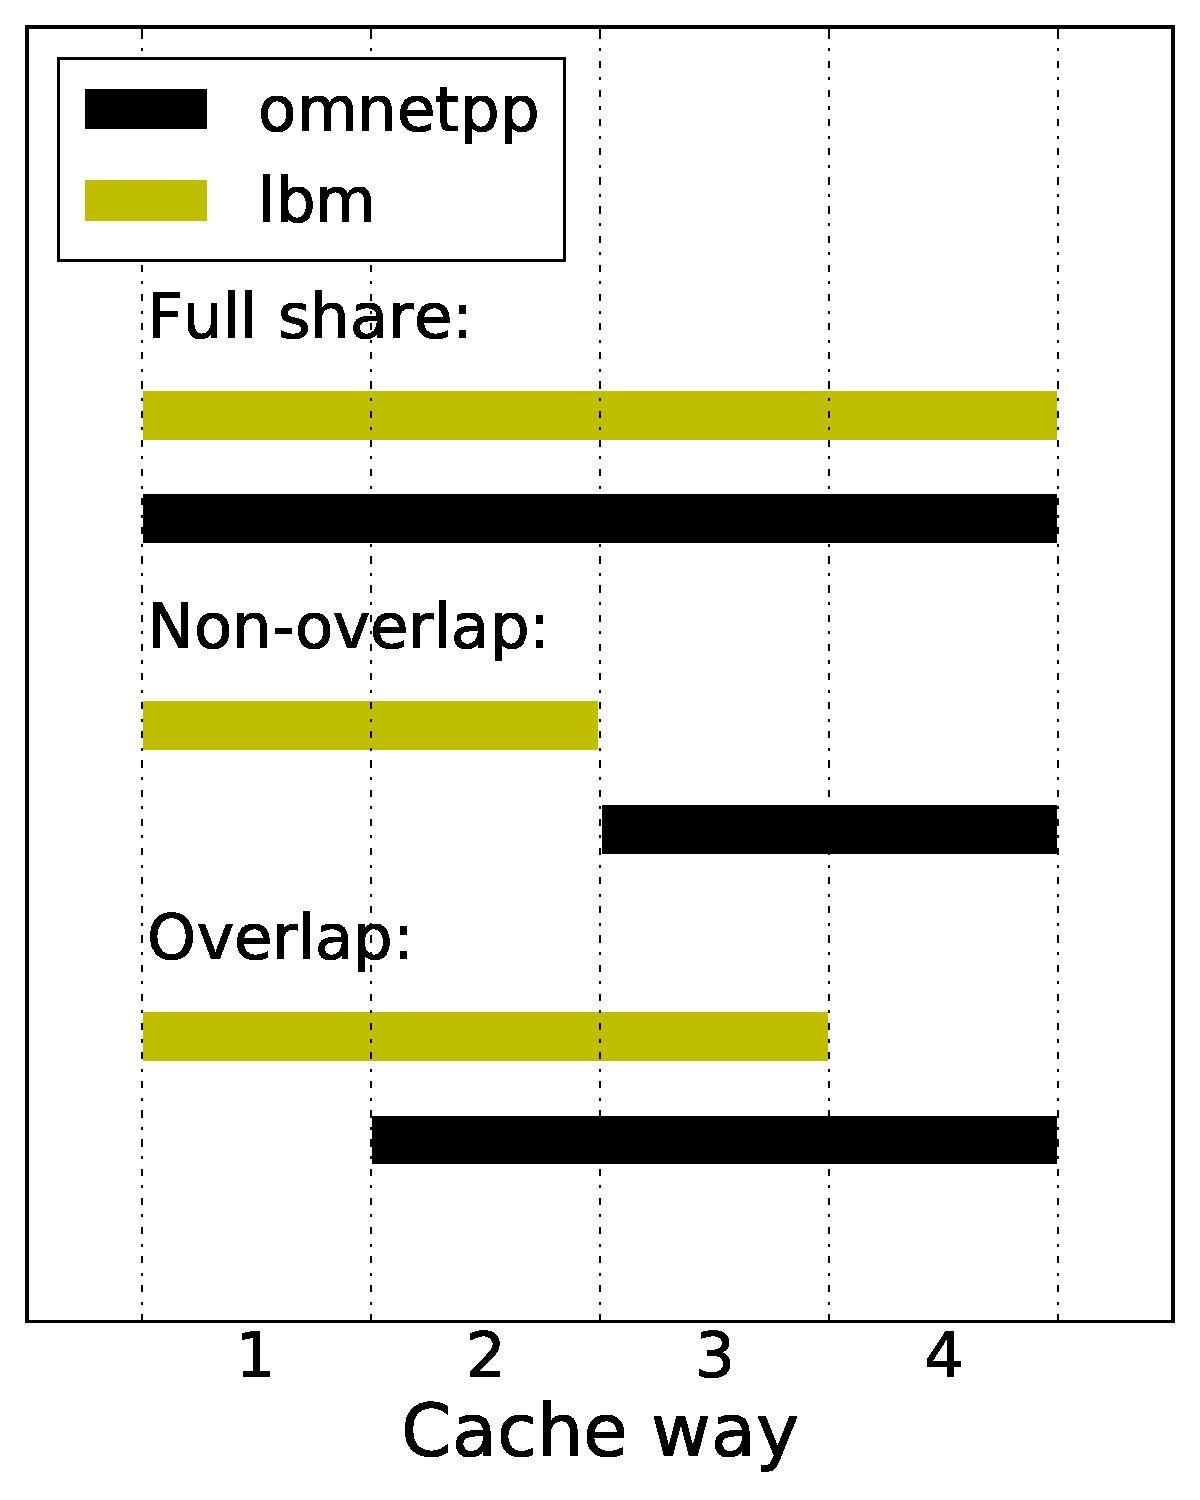
\includegraphics[width=0.9\linewidth]{figures/scheme.pdf}
        \caption{分配布局}
    \end{subfigure}%
    \begin{subfigure}[b]{0.4\linewidth}
        \centering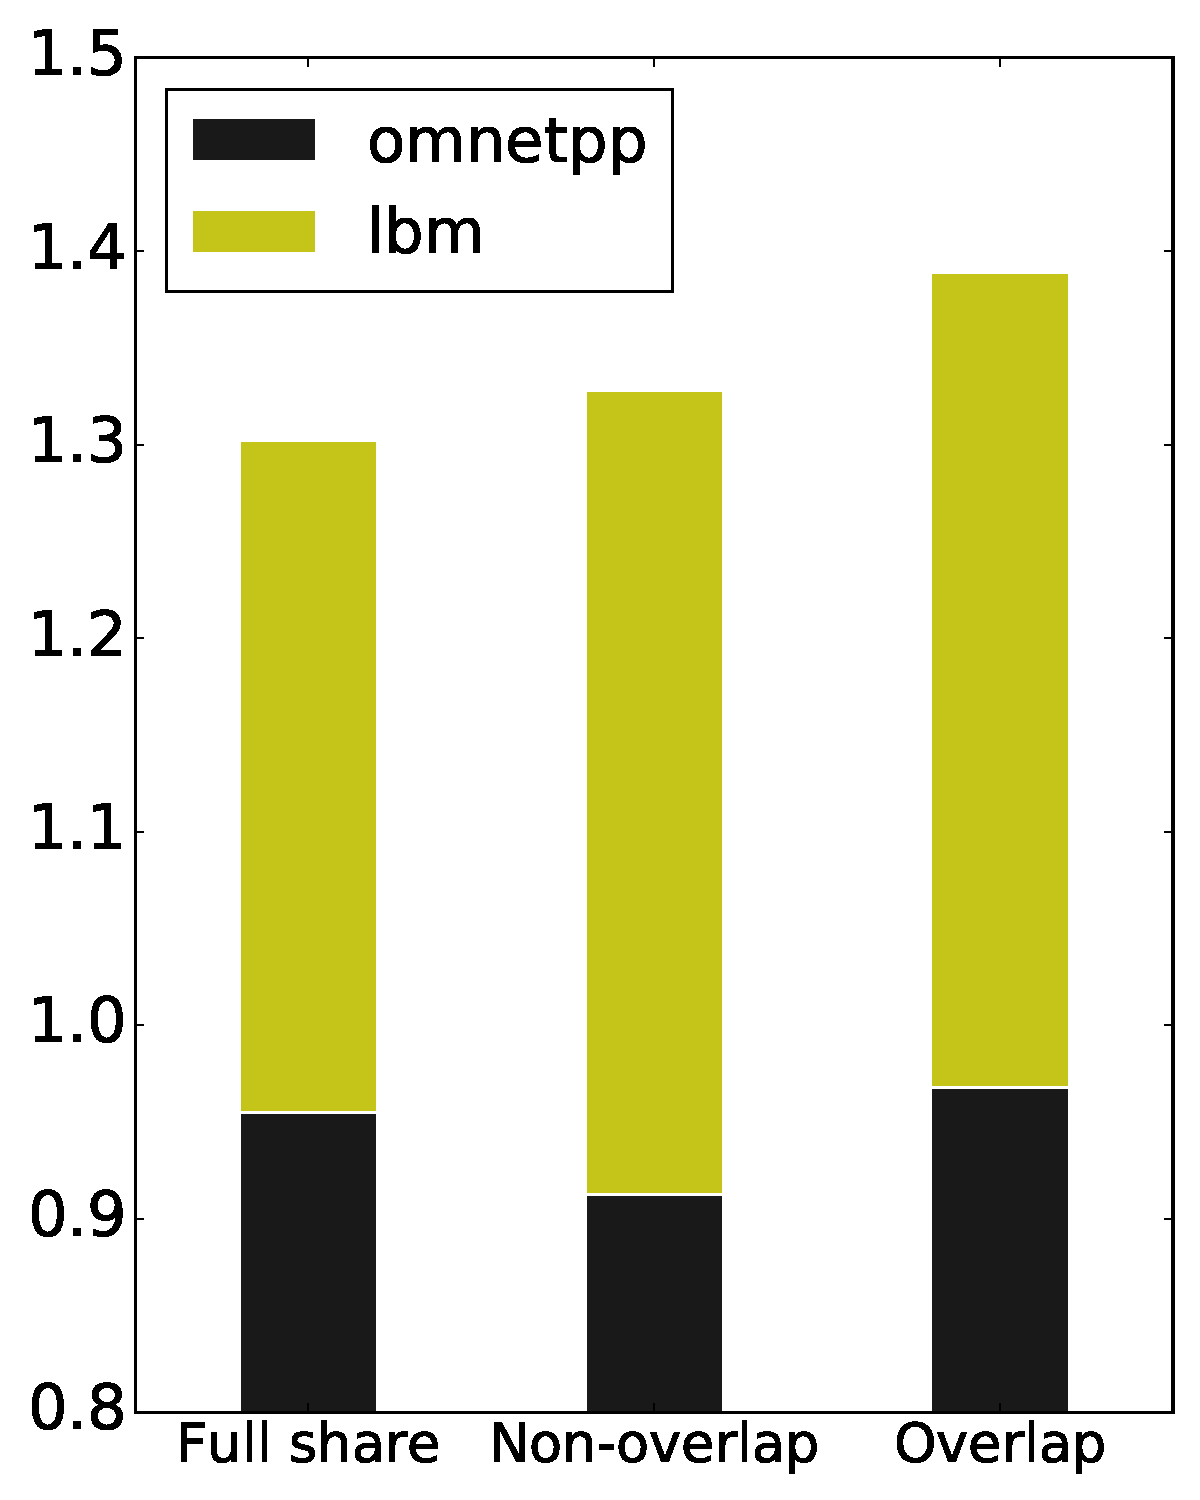
\includegraphics[width=0.9\linewidth]{figures/throughput.pdf}
        \caption{IPC吞吐量}
    \end{subfigure}
    \caption{完全重叠、不重叠和部分重叠方案的比较示例}
    \label{fig:illustration}
\end{figure}

我们更深入的研究表明,随着核数/并发线程数的增加,CAPS生成的部分重叠方案对完全重叠和不重叠划分的优势会愈发明显。CAPS包含两个部分:(1)一个预测模型可以较为准确地预测出在任意重叠CAT分配下(完全共享和不共享划分是两个特例)的并发程序的缓存失效率和IPC,(2)一个优化算法在给定一个优化目标后生成一个优化分配方案。借助于英特尔CAT技术,我们在真机上实现了CAPS并在实际系统中进行了实验评估。在评估实验中,我们把每个并发的程序都运行完毕,同时一些性能指标通过硬件性能计数器(Performance Counter)和高速缓存监控技术(CMT)来收集和记录。CAPS具有高度的灵活性,可以支持很多优化目标和策略。我们在CAPS上实现了5种策略分别锚定5个优化指标:(1)每个程序平均的1000指令失效数(Average MPKI);(2)IPC吞吐量(Throughput);(3)相比于独占缓存,每个程序平均的性能损失(Average Slowdown);(4)兼顾公平的性能损失(Fair Slowdown);(5)最大的性能损失(Maximum Slowdown)。实验结果表明,相比于自由竞争,在Average MPKI这个指标上,CAPS平均可以降低16.96\%的失效数,最好情况下可以降低23.1\%;对于Throughput,CAPS平均提升11.11\%,最好情况下提升高达31.3\%;对于Average Slowdown,CAPS在平均程度上可以减小性能下降8.16\%,最优情况下达到11.18\%;对于Fair Slowdown,平均可以被减小8.17\%,最好情况13.2\%;对于Maximum Slowdown,平均可以提升23.24\%,最好情况下高达33.42\%。

本文提出的CAPS缓存分配优化框架的主要特点和优势有以下几点:

\begin{itemize}
    \item 在细粒度上实现缓存分配。通过精确的控制分配重叠,CAPS突破了way-partitioning技术的分配粒度限制,实现了细粒度的控制,同时也没有带来额外开销。细粒度分配可以带来更好的优化效果。
    \item 支持多种优化策略。过往的研究对于不同的优化目标需要制定不同的策略,而在CAPS中,只需要简单地适配优化函数,就可以实现一个新的策略。这大大增强了优化的灵活性。
    \item 具有良好的可扩展性。随着线程数/核数的增加,可扩展性对于一个优化框架来说格外重要。过去的解决方案多是针对双核/双线程的情景,对于如今动辄十几个核的处理器就会力不从心。而CAPS对于核数少与多的情况都提供了良好的支持性。
    \item 可以在真实系统中实现。CAPS是一个纯软件的框架,通过CAT技术得以在真实系统上实现。相比于模拟器,我们在真机上可以进行更加充分的实验。同时,CAPS也更容易被应用到实际生产环境中。
\end{itemize}

据我们所知,CAPS是国内外第一个基于缓存分配技术在真实系统上实现的普适性缓存优化框架,它开创性地利用部分共享缓存空间来增强优化效果。本文的后续部分如下安排:

在第\ref{chap:related}章中,我们介绍了有关高速缓存的重要概念,CAT技术的背景知识,以及国内外相关工作的研究进展。

在第\ref{chap:prediction}章中,我们将重点介绍CAPS的性能预测模型。我们讲探讨该预测方法的基本原理,给出算法设计,并阐述实现中的关键点。

在第\ref{chap:allocation}章中,我们提出CAPS的优化算法。我们会阐述该算法如何在给定条件下生成一个优化算法,并给出算法伪代码。同时我们会对CAPS中实现的5个优化策略进行进一步分析。

在第\ref{chap:evaluation}章中,我们通过大量的实验对CAPS进行全方位的评估。评估先从平均的角度给出综合评估分析,再从个别实验样本的角度进行细致分析。

最后,我们在第\ref{chap:conclusion}章中,总结了全文的工作成果,并提出未来的研究方向。
	% 各章节。
	% Copyright (c) 2014,2016 Casper Ti. Vector
% Public domain.

\chapter{研究背景和目标} \label{chap:related}
\section{高速缓存的相关概念}
在本节中,我们将列举并解释在本文中出现的与高速缓存相关的一些重要概念。

\textbf{多级缓存}

因为内存访问的延迟较高,为了弥补CPU与内存之间的速度差异,现代计算机通常都采用了层
次化的高速缓存架构,我们称之为多级缓存(Multi-level Cache)。按照缓存距离CPU 的远近,依次将其称为L1、L2、L3 等。特别的,我们将体系结构上最远离CPU、存取速度最慢的那一级称为底层缓存(Last-Level Cache,LLC),其余的统称为高层缓存(Higher Level Cache)。在多核处理器中,每个处理器核(Core)通常具有各自独立的高层缓存,我们将它们称为核的私有缓存(Private Cache)。底层缓存却通常被多个核(甚至所有核)所共享,我们称其为共享缓存(Shared Cache)。这种设计既有助于在一定程度上保证核与核之间的隔离,同时又能使各个核在底层缓存上进行高效的数据交换,并简化处理器的硬件复杂度。

在多级缓存中,如果某级缓存所存储的数据同时存在于其下一级缓存中,我们就将这下一级缓存称为包含型缓存(Inclusive Cache)。反之,如果在同一时刻相邻两级缓存中没有重复的数据单元,我们就将较低的那级缓存称为排除型缓存(Exclusive Cache)。尽管包含型缓存造成了一定的空间浪费,但却有助于提高缓存同步(Cache Coherence)时的性能。这是因为如果发现要同步的数据不在该缓存中,我们就没有必要把同步操作再向上层传递。而且,对于共享的包含型缓存,我们还可以在其缓存单元中记录该数据还存放在哪些私有缓存中,而避免向所有上层缓存发出请求。所以,目前的商用处理器多采用包含型缓存的设计。

如图\ref{fig:cache_hierarchy}所示是一个典型的多级缓存设计,英特尔近年的微处理器架构,包括都Sandy Bridge、Haswell、Skylake,都采用了这一设计。每个处理器核拥有两层独立的私有缓存,第一层私有缓存包括L1 D-cache和L2 I-Cache,分别负责数据和指令缓存;第二层私有缓存L2 Cache。L1、L2缓存每个核都有且独占。底层缓存LLC,也可以被称为L3 Cache,为所有核所共享。

\begin{figure}[htbp] 
    \centering
    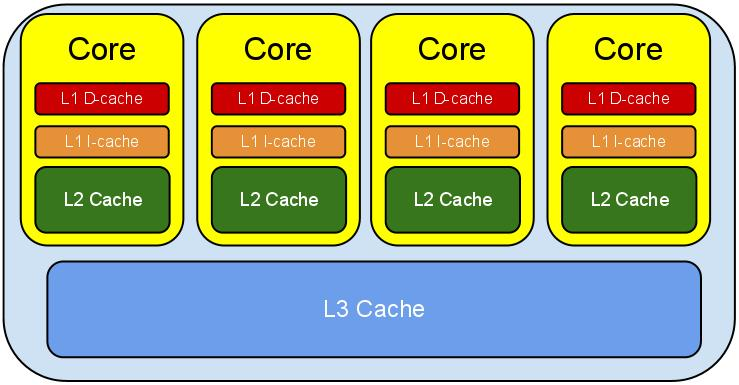
\includegraphics[width=0.8\linewidth]{figures/CacheHierarchy.jpg}
    \caption{多级缓存的示例}
    \label{fig:cache_hierarchy}
\end{figure}


\textbf{相联度}
缓存中一个最小的存储单元称为缓存块(Cache Line)。缓存的相联度(Associativity)决定了某个内存地址的数据能存放在哪些缓存块中。

相联度为1的缓存称为直接映射缓存(Direct Mapped Cache)(图\ref{fig:cache_asso}(a))。对于直接映射缓存,硬件会将内存地址的一部分作为索引,将其对应到一个唯一的缓存块。因此,每块内存数据都只能存放在一个特定的缓存块中,而如果两个内存地址的索引部分相同,就将导致冲突(Conflict)。

如果缓存的相联度和缓存块的总数相同, 则称之为全相联缓存(Full Associative Cache(图\ref{fig:cache_asso}(b))。在全相联缓存中,一个内存地址能缓存在任何一个缓存块中,硬件通过全相联比较器确定该内存地址被缓存的位置。全相联缓存能够使缓存空间得到更有效的利用,但却需要极大的硬件复杂度。

组相联缓存(Set Associative Cache)是以上两种类型的混合(图\ref{fig:cache_asso}(c))。它按照相联度将缓存块平均分为若干缓存组(Set),同组内的各缓存块称为路(Way),路的数目就是缓存的相联度。分配缓存时,硬件首先根据内存地址的一部分确定该数据所对应的缓存组,数据可以缓存在该组内的任何一个缓存块中。硬件设计人员可以通过控制相联度,在冲突失效率及硬件复杂度之间做出权衡。现代处理器多采用这种设计。

\begin{figure}[htbp] 
    \centering
    \begin{subfigure}[b]{0.24\linewidth}
        \centering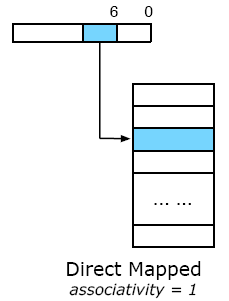
\includegraphics[width=0.9\linewidth]{figures/CacheAsso1.png}
        \caption{直接映射}
    \end{subfigure}%
    \begin{subfigure}[b]{0.24\linewidth}
        \centering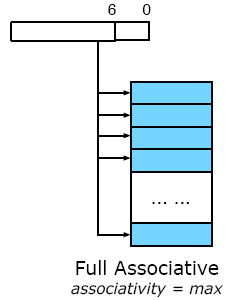
\includegraphics[width=0.9\linewidth]{figures/CacheAsso2.png}
        \caption{全相联}
    \end{subfigure}%
    \begin{subfigure}[b]{0.52\linewidth}
        \centering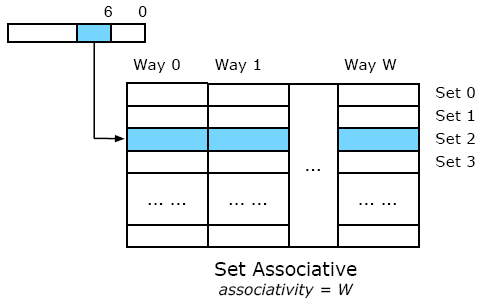
\includegraphics[width=0.9\linewidth]{figures/CacheAsso3.png}
        \caption{组相联}
    \end{subfigure}
    \caption{缓存的相联度}
    \label{fig:cache_asso}
\end{figure}

\textbf{管理策略}
为了管理全相联缓存和组相联缓存中自由的缓存空间,硬件通常以队列的逻辑形式来组织这些缓存块。当缓存失效(Cache Miss)时,新数据将插入队列的什么位置取决于缓存的插入策略(Instertion Policy)。当要缓存的内容超过缓存容量时,硬件就会按照某种策略从队列中淘汰一个缓存块,这个策略称为替换策略(Replacement Policy)。当缓存命中(Cache Hit)时,如何调整命中的缓存块在队列中的位置取决于缓存的晋升策略(Promotion Policy)。

由于局部性原理,最近最少使用(Least Recently Used,LRU)是最为被广泛使用的缓存队列组织形式。在LRU 队列中,我们将队首的位置称为MRU(Most Recently Used),将队尾的位置称为LRU。那么其管理策略就可以概括为:新数据插入到MRU 的位置,从LRU 的位置淘汰数据,命中的数据将晋升到MRU的位置。

由于程序的数据访问在时间和空间上会有局部性的特性,即如果一个信息项正在被访问,那么在近期它很可能还会被再次访问;以及在最近的将来将用到的信息很可能与现在正在使用的信息在空间地址上是临近的。所以LRU策略可以提供较好的缓存管理效率。严格的LRU在实现上比较困难,且会带来较大的额外开销,所以现代处理器多采用近似LRU的管理策略。

\section{缓存划分的相关研究}
在LRU策略下的共享缓存LLC中,不管访问来源与哪个核都被一视同仁,也就是说所有核在竞争使用LLC。然而,竞争的结果往往不是效率最高的结果。因为某些高污染程序,比如流媒体应用,往往会占据大量的缓存资源,从而导致同时运行的其他程序因为没有足够的缓存而性能下降。如何高效地管理和优化共享缓存是学术界非常关心的一个问题。优化共享缓存的一个关键点就是通过缓存的划分,来改善系统的整体性能。我们广泛调研了关于缓存划分技术的相关研究,将其归纳为硬件技术和软件技术两大类。

\textbf{硬件技术}
基于硬件的研究主要通过改良缓存硬件、优化缓存管理策略等方法来完成缓存的优化。

Suh等首先提出了动态缓存划分的思想来优化共享缓存的利用率~\parencite{suh2002new,suh2004dynamic,suh2014analytical}。他们采用了一种软硬件结合的方法,首先由修改过的硬件动态构造出一个失效率曲线,然后操作系统利用该曲线求出使得总失效率最低的一种划分方案,最后再由CPU通过修改缓存替换策略完成缓存分割。这种方法带来了很大的硬件开销。

Qureshi等对上述方法加以改进~\parencite{qureshi2006utility,qureshi2007adaptive},他们将增加单位缓存后某个程序减少的失效数称为效用(Utility),并实现了以最大化全局效用为目标的缓存划分方法。其主要优化包括:为每个核构造单独的失效率曲线图,以提高决策的准确度、用组采样(Set Sampling)来降低硬件开销,以及优化寻找最优划分的贪心算法。试验表明,该方法能够用较小的硬件开销实现平均情况下11\%的性能提升。

Rafique等给出了一种通用的、让操作系统自由控制缓存配额的软硬件接口
~\parencite{rafique2006architectural}。他们设计了该接口的体系结构支持,并在模拟器上评测了若干策略。他们认为,这种策略与机制相分离的方法具有更强的适用性。

Srikantaiah等提出了一种自适应组独占(Adaptive Set Pinning)的方法~\parencite{srikantaiah2009sharp}。它能自动根据需要,将某些缓存组分配给某个处理器核独占使用一段时间,从而同时减少核与核间由于同步操作导致的缓存失效,以及处理器核自身由于容量限制或地
址冲突导致的缓存失效。

Xie 等提出了一种称为PIPP的缓存“伪划分”技术~\parencite{xie2009pipp}。他们首先用Qureshi 的方法得到一个最优的划分方案,再通过调整缓存的插入策略和晋升策略,使缓存的分配动态平衡在想要的划分比例。他们的实验结果表明,这种方法避免了刚性划分所引起的缓存空间利用不当,能够综合Qureshi工作的优点。

此外,还有一些研究针对不同的优化目标。Iyer等提出了基于服务质量(Quality of Service, QoS)的优化模型。针对多核平台下任务多样性的新趋势,QoS 存储架构能够根据应用的优先级,可控地分配缓存空间和内存带宽等资源~\parencite{iyer2004cqos}。Kim 等提出了以性能公平性(Fairness)为目标的共享缓存管理策略~\parencite{kim2004fair}。Hsu等总结了基于性能、服务质量以及公平性这三方面的优化目标~\parencite{hsu2006communist},并提出相应的优化策略。

上述这些研究,虽然在优化目标、策略及算法上有所不同,但实现缓存划分的方式都是基于路的划分(Way Partitioning)。路划分技术是将缓存的路(Way)分配给各个核,它的最小划分单位为一个缓存路。之所以路划分技术被广泛使用是因为其设计简单,不需要很复杂的硬件修改。但是它的不足之处在于分配的粒度较粗,一个路往往会有很多缓存块,这在核数较多时会显得力不从心,因为最优划分很可能会且在一个路的中间。对于一个处理器而言,缓存的路数在设计之处就已经确定,而且数目不会太多,当核数增加时,分配的灵活性将会大大下降。当核数等于路数时,每个核有且只能被分配一个路,这就彻底失去了灵活性,只能起到隔离的效果。

一些研究试图改进路划分技术,提高分配粒度。Chang等提出了称为CCP共享缓存的技术~\parencite{chang2006cooperative,chang2014cooperative}。这种方法从时间和空间两个维度上分配共享的缓存资源。它可以通过控制处理器核使用某个缓存分区的时间片长短来保证公平性,并通过伸缩每个缓存分区的大小来控制服务质量。通过时间共享来细化划分粒度。Manikantan提出了PriSM通过精确地控制缓存失效概率来细化分配粒度~\parencite{manikantan2012probabilistic}。还有一些研究抛弃了路划分,采用更加复杂的硬件设计来实现细粒度缓存分配~\parencite{sanchez2011vantage}。

所有的硬件研究因为涉及到硬件修改,所以基本都是在模拟器中进行。

\textbf{软件技术}
软件方面主要依赖于“页面着色”(Page Coloring)这一技术。Lin等首先提出了“页面着色”技术~\parencite{lin2008gaining},在Linux 操作系统上实现了无需硬件支持的缓存分区,它们提出了一种按照失效率和敏感度对应用程序使用缓存的特征进行分类方法,并利用该方法设计了若干组基准程序,评估了页面着色方法对他们的效果。之后多个学者对这一技术进行了更深入的研究和应用~\parencite{zhang2009towards,soares2008reducing,tam2007managing,azimi2009enhancing,lu2009soft}。

页面着色的基本原理是通过操作系统控制页面到缓存块的映射,从而限制缓存被分配的区域。这种技术可以在真实系统上通过软件实现,而且原则上来说可以将分配粒度细化到一个缓存块。然而,目前处理器纷纷采用哈希算法映射物理地址到缓存块,而不是过去的一一对应。在不知道哈希函数的情况下,就无法通过页面着色来控制缓存块的分配。所以现在页面着色技术已经不再适用。

\section{英特尔高速缓存分配技术}
英特尔在2016年发布的第四代至强处理器产品家族中全线引入了资源调配技术(RDT),高速缓存分配技术(CAT)是其中重要的组成部分。高速缓存分配技术首次在商用处理器上实现了对共享缓存(LLC)容量的管理。通过CAT技术,我们可以在软件层面为每个核分配可使用的缓存资源。下面我们简要介绍CAT的使用方法。

CAT通过一个被称为CLOS(Class of Service)的单元来控制缓存的分配。每个CLOS包含一个CBM(Capacity Bitmask)的容量掩码,代表该CLOS可以使用哪些缓存。CBM是由一串连续的1构成01串,1代表当前位这一路的缓存可以被适用,0代表不能被使用。将处理器核与某个CLOS绑定,该核就只能占用被CLOS中的CBM所指定的缓存。

图 \ref{fig:CLOS}是一个CLOS与CBM的例子。CLOS[0]分配有第19到第16路的缓存,CLOS[1]分配有第15到第12路缓存,CLOS[2]分配有11到第6路缓存,这一部分与CLOS[3]发生了重叠。一个核与某个CLOS绑定后就会受到其限制了。

\begin{figure}[htbp] 
    \centering
    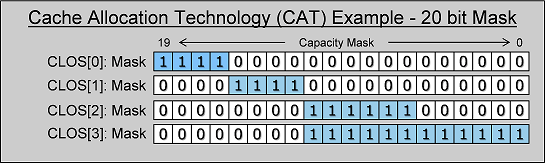
\includegraphics[width=0.8\linewidth]{figures/CLOS.png}
    \caption{CLOS与CBM的示例}
    \label{fig:CLOS}
\end{figure}

CAT借鉴了前人的研究成果,采用了路划分(Way Partitioning)技术这一设计。前人在模拟器中可以调整缓存路数,然而真实处理器中的路数是固定的。CAT可分配的路数非常有限,在最高端的CPU中仅有20路可供分配,每一路高达几兆字节的缓存空间,所以说CAT的分配粒度很粗。

此外CAT技术与以往的技术有两点很大的不同:
\begin{itemize}
\item 分配必须是连续的。CBM必须包含连续的1,例如,“0111”是一个有效的分配,而“1011”则不行。
\item 分配间允许重叠。例如,可以把“1110”分配给一个核,“0111”分配给另外一个核,中间两路缓存两个核所共享。
\end{itemize}

这两个特点意味着在CAT中分配的位置也需要被考虑。以往的研究通常只需要考虑分配“多少”缓存,因为分配不一定要连续而且不会重叠。而CAT中因为连续的要求和允许重叠,所以分配在“哪里”也同样重要。

目前关于CAT的研究都集中在QoS方面~\parencite{lo2015heracles, herdrich2016cache, funaro2016ginseng}。它们主要通过提供给高优先级的程序足够的缓存资源来满足QoS要求,而让低优先级程序共享剩余的缓存。这种思路并不需要细粒度的缓存控制,所以CAT可以轻松胜任。

\section{研究目标}
随着处理器中的核数越来越多,共享缓存的竞争问题也愈发严重。目前,还没有一个可以在真实系统上可以运行的缓存优化框架,我们希望通过我们的努力实现这样一个框架的原型。我们称之为CAPS,它可以满足以下几个方面的要求:(1)\textbf{可以在真实系统中运行};(2)\textbf{实现细粒度分配控制};(3)\textbf{良好的可扩展性,在核数较多时依然有很好的适应性};(4)\textbf{具备灵活性,支持多种优化策略}。

共享缓存分配优化的步骤一般包含以下三步:
\begin{enumerate}
\item 预测。首先需要在任意分配情况下,对每个并发程序的性能进行预测和评估。性能参数包括失效率(Miss Rate)和周期指令数(IPC)等等。预测的指标用来为后面的决策提供参考依据。
\item 决策。根据预测的指标,和优化目标,做出一个分配决策。针对不同的优化目标,可能会采取不同的策略和算法。
\item 实施。将决策的分配付诸实践,让分配真正产生效果。
\end{enumerate}

若要在真实系统上实施分配,CAT技术是目前唯一的方法。所以CAPS必须倚仗于CAT作为最后实施分配的方法。而分配技术对前两个步骤,即预测和决策又有深远的影响,因为决策所得到的分配必须符合分配技术的要求,而预测又是为决策所服务。如上节所述,CAT技术要求分配必须连续以及有限的可分配资源都为实现细粒度、可扩展和灵活的分配优化带来了极大的困难。然而,CAT允许重叠这一特性却带来很大的操作空间。虽然重叠分配,尤其是部分重叠,为预测模型和分配决策带来了更大的挑战,但是我们通过研究探索,在CAPS中实现了一个全新的预测模型,以及一个基于模拟退火的决策算法,可以支持部分重叠下的CAT分配的性能预测和优化决策,让上述提出的四点目标得以满足。在下一章中,我们将首先介绍CAPS预测模型。


	% Copyright (c) 2014,2016 Casper Ti. Vector
% Public domain.

\chapter{CAPS设计与实现} \label{chap:design}
\section{CAPS综述}
随着处理器中的核数越来越多,共享缓存的竞争问题也愈发严重。目前,还没有一个可以在真实系统上可以运行的缓存优化框架,我们希望通过我们的努力实现这样一个框架的原型。我们称之为CAPS,它可以满足以下几个方面的要求:(1)\textbf{可以在真实系统中运行};(2)\textbf{实现细粒度分配控制};(3)\textbf{具有良好的可扩展性,在核数较多时依然有很好的适应性};(4)\textbf{具备灵活性,支持多种优化策略}。

共享缓存分配优化的步骤一般包含以下三个过程:
\begin{enumerate}
\item 预测过程(Prediction)。首先需要在任意分配情况下,对每个并发程序的性能进行预测和评估。性能参数包括失效率(Miss Rate)和周期指令数(IPC)等等。预测的指标用来为后面的决策提供参考依据。
\item 决策过程(Decision-making)。根据预测的指标和优化目标,做出一个分配决策,给出优化分配方案。针对不同的优化目标,可能会采取不同的策略和算法。
\item 执行过程(Enforcement)。通过某种技术实施优化分配分配方案,让分配真正产生作用。
\end{enumerate}

若要在真实系统上实施分配,CAT技术是目前唯一的方法。所以CAPS必须倚仗于CAT作为执行分配方案的技术。而采用哪样的分配技术对前两个步骤,即预测和决策过程,又有深远的影响,因为决策所得到的分配必须符合分配技术的要求,而预测又是为决策提供服务。如上一章所述,CAT技术要求分配必须连续,有限的可分配路数的情况下,要实现细粒度、可扩展和灵活的划分是非常困难的。然而,CAT允许分配之间重叠的这一特性却带来很大的操作空间。虽然在分配重叠,尤其是部分重叠,会给预测模型和分配决策带来了更大的挑战,但是我们通过研究探索,在CAPS中实现了一个全新的预测模型,以及一个基于模拟退火的决策算法,可以支持部分重叠下的CAT分配的性能预测和优化决策,让上述提出的四点目标得以满足。

CAPS框架的整体架构如图\ref{fig:caps_overview}所示。首先,需要对并发工作负载中的每个程序进行一次离线采样分析,分析得到该程序的缓存特征,包括缓存失效率曲线(MRC),以及访存频率(API)。离线采样分析只需要进行一次即可,结果被保存在硬盘中以便之后使用。CAPS最重要的两个模块是预测模型和优化算法。预测模块可以对任意CAT分配下,包括部分重叠的分配方案,对每个程序的性能进行预测。预测指标包括缓存失效率(Miss Rate)和周期指令数(IPC)。优化算法依赖于预测模块,它通过模拟退火算法,在CAT分配方案的解空间中进行启发式搜索,对于每个可行解调用预测模块进行预测,再根据预测结果找到一个最优分配方案。最后,通过CAT技术实施这一方案。

\begin{figure}[htbp] 
    \centering
    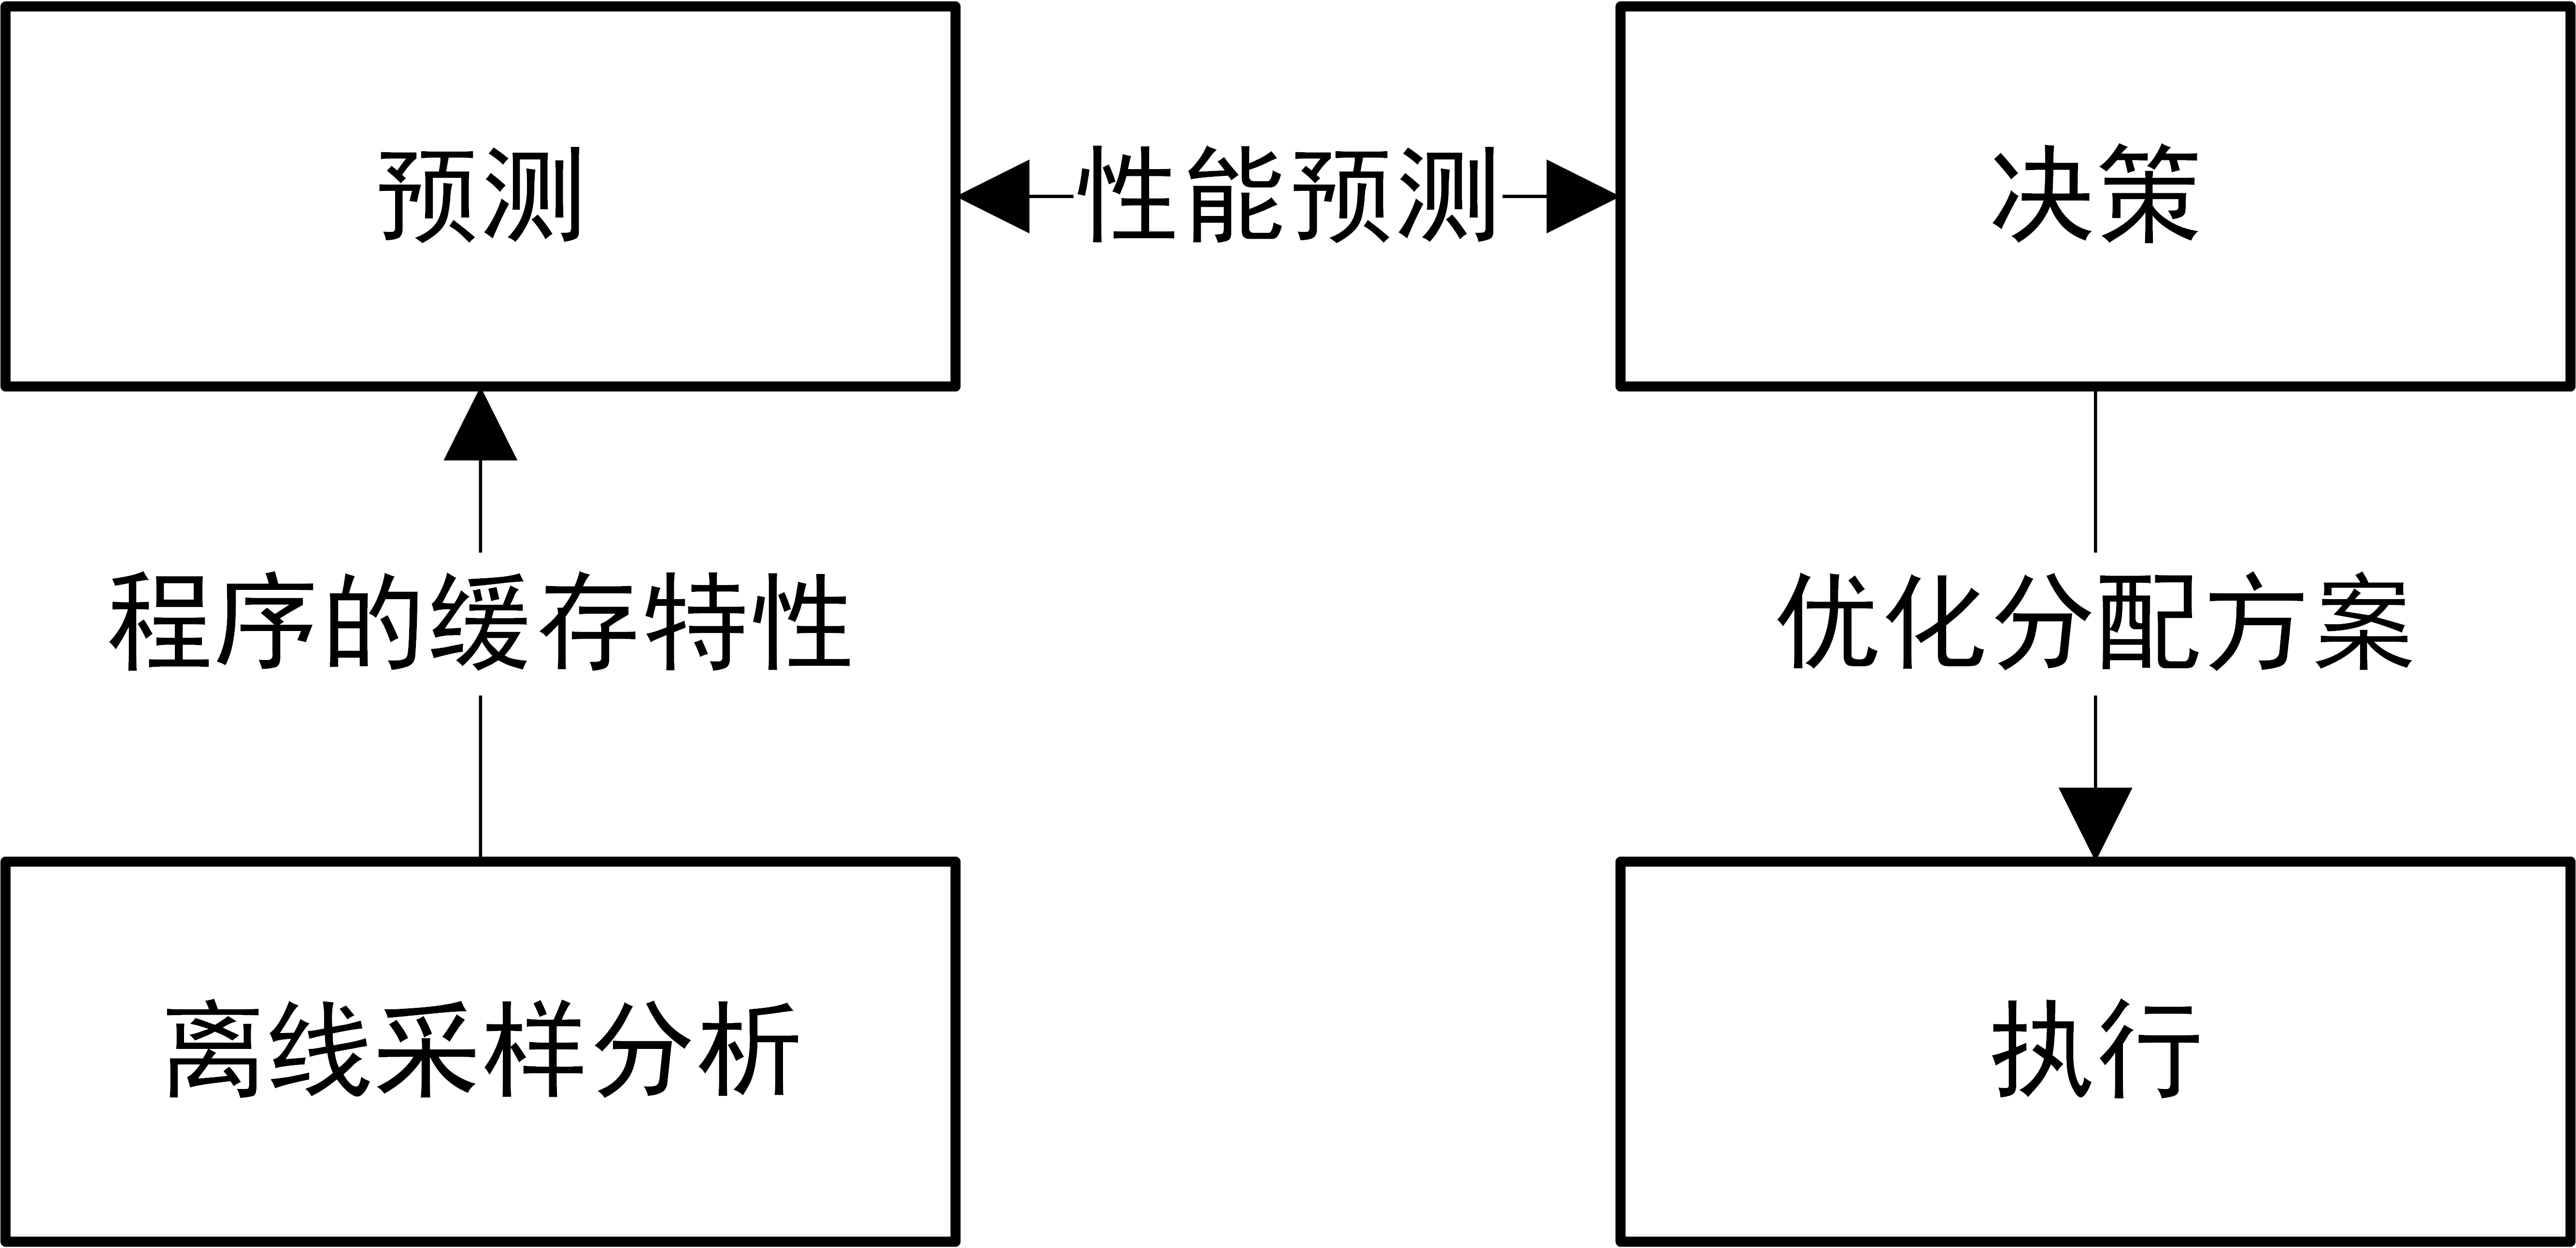
\includegraphics[width=0.6\linewidth]{figures/caps_overview.png}
    \caption{CAPS架构}
    \label{fig:caps_overview}
\end{figure}

CAPS框架两个最重要的模块是预测模型和优化算法。在给定一个优化目标后,预测模块与优化模块两者相互协作,在较短时间内可以生成一个优化分配方案。同时CAPS还具有良好的可扩展性,支持多种多样的优化目标。我们在本文中实现了5种优化指标及相应的策略,这些目标分别侧重性能、公平性以及服务质量(QoS)等不同的方面。经过我们在真机上的实验评估,无论在哪个优化指标下,CAPS都能起到良好的优化效果。

\section{预测模型} \label{sec:prediction}
\subsection{模型概述}
在本章中,我们将介绍CAPS的预测模型。对缓存失效率的预测是优化的基础,它的准确性会直接影响到整个优化框架的效果。由于优化决策依赖于预测模型提供的信息,不准确的预测结果可能会导致错误的分配决策。虽然前人对失效率预测进行了大量工作,但它们都不适用于CAT下的预测,因为前人的研究都没有考虑过分配间部分重叠的情况。为了应对部分重叠的问题,我们为CAPS推导了一个全新的预测模型。

CAPS预测模型可以较为准确地预测出,多个并发执行的程序在任意CAT分配下,每个程序的缓存失效率(Miss Rate)和周期指令数(IPC)。一个CAT分配包括每个线程/核的分配(CLOS)的集合。CAPS预测模型的输入包括每个并发程序的失效率曲线(Miss Rate Curve,MRC)和访存指令占比(Accesses per Instruction, API),以及加载于它们身上的CAT分配。MRC和API可以描绘出一个程序的局部性和缓存访问频率等特征,这两个指标都可以通过离线采样分析得到,在第\ref{sec:prediction_sample}节中会详细介绍。MRC刻画了失效率随缓存大小变化的情况,它是描述某个程序的缓存敏感度的一种有效手段。MRC是这样一条曲线,它的横轴是缓存占用,纵轴是失效率。API用来刻画程序的访存频率,它代表了程序对缓存的污染程度,通常访存频率越高,在与别的程序竞争中越有优势。

CAT技术规定,一个程序的分配可与一个或多个其他程序的分配重叠。重叠的部分就意味着有不止一个程序会竞争使用这一缓存区域。对于独占的缓存区域,程序的缓存占用就是分配的大小,而对于共享区域,每个程序实际占用的缓存大小就不是一目了然了。预测的关键问题就在于弄清楚这些重叠部分的竞争结果,即程序在竞争下实际得到的缓存大小。我们通过一个迭代算法解决了这一问题,算法会在第\ref{sec:prediction_iteration}节中详细阐述,简而言之,该算法通过迭代过程找到均衡状态时每个程序的实际占用,每次迭代相当于一小段程序执行周期,在这个过程中,它们的缓存占用发生了改变。我们假设每个程序的访存模式都是稳定的,所以在均衡状态下,各个程序的缓存占用也会达到稳定,这个稳定值就是我们要求的答案。根据真实占用和MRC很容易推导出每个程序的失效率,再根据失效率估计出IPC,就得到了模型的输出。值得一提的是,实际中每个程序的访存模式都会随着运行阶段的变化而变化,CAPS预测模型也可以适应于这种变化,但是需要实时地获取MRC。在本文中,我们只关注程序的平均性能,所以只使用离线采样的平均MRC和API作为输入。

在我们对4到15个程序的工作负载进行了多达750次实验,结果表明CAPS预测模型具有较高的预测准确率,同时还能保持较低的额外开销,具体的实验评估见第\ref{chap:evaluation}章。


\subsection{离线采样分析} \label{sec:prediction_sample}
本节中,我们将介绍如何通过PIN这一工具离线采样得到程序的MRC和API。研究者们对于如何获取MRC进行了大量的研究,在CAPS中,我们借鉴了基于平均淘汰时间(Average Eviction Time,AET)的技术~\parencite{hu2016kinect}。任何MRC采样技术都需要程序的访存序列,它是构建MRC的基础。在本文中,我们使用PIN~\parencite{luk2005pin}这一工具对访存序列进行追踪。

Pin是一款针对x86 指令系统的二进制代码分析工具(Binary Instrumentation Tool)。它能够在不改变原有程序执行逻辑的前提下,在该程序的任何指令前后插入用户自定义的代码片段。Pin 包含引擎(PinEngine)和工具(PinTools)两个部分。PinEngine是一个不开源的可执行程序,是其核心部分,它负责完成二进制代码解析和改写。PinTools是由用户自己编写的一些函数库,定义了代码替换的具体规则、以及要插入的代码片段。当Pin执行时,PinTools 会以模块的形式被动态链接到PinEngine中,二者协同完成整个代码替换。

Pin与AET结合构建MRC的工作流程如下:
\begin{enumerate}
\item 被测试的基准程序作为输入被Pin引擎读入翻译缓存,PinEngine对它的二进制代码进行静态分析,标记出函数、基本块等;
\item 完成一批代码分析后,PinEngine会自动调用PinTools中注册的代码替换回调函数(Instrumentation Callback)。该函数根据用户自己的需要,扫描Pin分析出来的指令流,再调用PinEngine提供的代码替换接口,将自定义的指令回调函数(Execution Callback)插入到程序的指令流中。本例中,我们在所有访存指令之前加入了自己的代码memop(ip, ea);
\item PinEngine将修改后的代码片段载入其执行缓存,并跳转执行它。
\item 执行到访存指令时,修改后的代码片段自动调用先前插入的指令回调函数memop(),且PinEngine会计算出该指令的指令指针ip和被访问的内存地址ea,作为参数传递给回调函数。回调函数memop()的行为非常简单,它将内存地址ea这个参数以二进制的方式写入Memory Trace文件中。
\item 当被测试的基准程序执行完毕或执行到指定时间后,将Memory Trace文件作为输入AET模型进行失效率曲线MRC构建。
\item AET模型计算完毕后,输出失效率曲线MRC。
\end{enumerate}

\begin{figure}[htbp] 
    \centering
    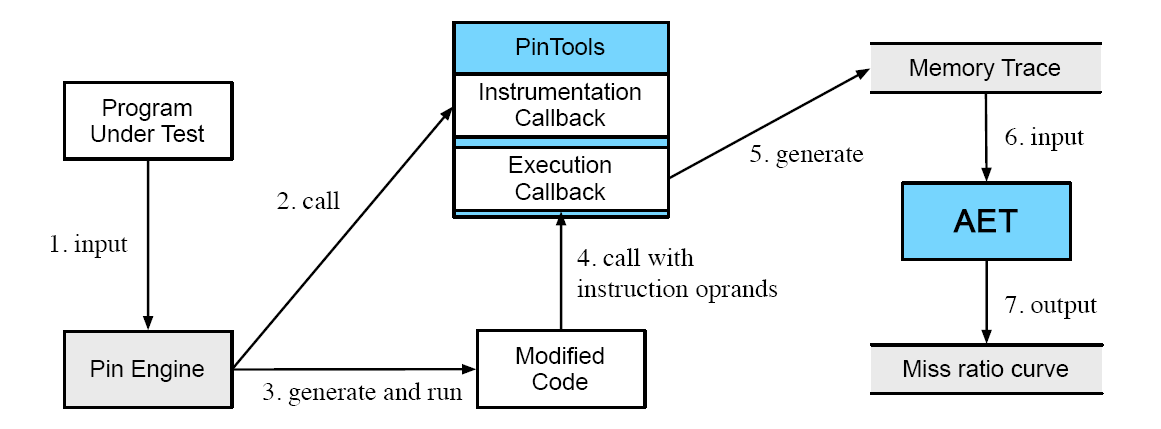
\includegraphics[width=0.8\linewidth]{figures/pin.png}
    \caption{利用Pin和AET构建MRC的流程图}
    \label{fig:pin}
\end{figure}

AET是一个先进的MRC采样技术,它可以在较低的时间空间开销下根据访存序列得到一个准确的MRC。虽然额外开销对于离线优化框架来说并没有那么重要,但我们仍然想控制时空开销,因为我们计划在未来将CAPS拓展到在线环境中。AET具有线性的时间复杂度,并且可以通过随机采样来减少运行时间,同时也能保持较高的MRC准确率。

以往的MRC技术多是基于重用距离,它被定义为对同一数据的相邻两次访问间所间隔的不同数据数。通过构造出重用距离直方图,然后累加得到MRC。但是完整地统计出重用距离直方图会带来巨大的时间和空间开销。从渐进意义上来说,对于$N$个读写访问到$M$个不同的地址,构造重用距离直方图的时间复杂度为$O(N\log M)$,空间复杂度为$O(M)$~\parencite{olken1981efficient}。

基于AET的方法引入了平均淘汰时间(Average Eviction Time,AET)这一概念。失效时间(Eviction Time)被定义为最近一次访问到失效所经历的时间。LRU缓存可以被看作是一个栈,栈中数据按最近访问时间排序。最近访问多的在栈顶,最近访问少的在栈底。栈底被挤出去的就是被替换掉了。AET实际上就是缓存块从栈顶移动到栈底并出栈的平均时间。AET模型的输入是重用时间而不是重用距离,两者的差别在于,前者并不需要统计两次重用之间不同的访问次数,只需要统计总次数,所以可以通过随机采样的方式大大减少时间和空间消耗,因为只要采样的重用时间分布与真实的分布一样,AET一样可以得到准确的MRC。通过随机采样一小部分的访存,大量的时间和空间开销可以被节省下来。然而,对于部分共享的情况,只有MRC是不够的,下一节我们将介绍如何通过一个迭代算法来求解重叠情况下的预测问题。

% 在步骤6 中,计算重用距离需要知道与上次访问该地址之间间隔的不同地址的
% 数目。这需要用一个散列表记住所有访问过的内存地址,然后用链表将它们串起,
% 在软件中模拟LRU 队列的行为。由于程序的访存操作数以百亿计,优化这一算法
% 是十分必要的。本文采用了文献[56]中提到的树算法来加速重用距离的近似计算。

\subsection{迭代预测算法} \label{sec:prediction_iteration}


在分配没有重叠的情况下,系统给定的分配大小就是该程序缓存占用的的实际大小,根据MRC就可以直接得到失效率。然而,在分配重叠的情况下,问题就变得复杂了。有一些研究针对完全重叠的情况进行预测~\parencite{chandra2005predicting, suh2014analytical, xiang2011all, xiang2011linear, hu2016kinect}。但是,这些研究对于我们所面对问题,即部分重叠分配的预测,都无能为力。简单地把部分重叠分配下的每个完全重叠片段看成是一个自由竞争的小缓存块是不正确的。因为CAT是通过缓存失效来驱动的,在CAT下,如果是一个缓存命中,那么它可以命中在LLC的任何地方,即使是在这个核的分配之外,此时CAT不发挥作用。CAT只在缓存失效时才发生作用,CAT限制了该缓存失效只能替换掉分配区域内的一个缓存块。所以,对于处理器核来说,它发出的访问请求并不是均匀分布在它的分配中,而是它引起的失效均匀分布到它的分配中。因此,我们不能把每个重叠的缓存片段当成一个独立的完全共享的缓存,所以之前很多对于完全共享缓存的研究不能套用到部分共享的情况下来。

为了解决部分共享下失效率的预测问题,我们推导了一个全新的模型,通过一个迭代算法来预测部分共享缓存的情况下各个程序的缓存占用和失效率。首先,我们根据每个分配的起点和终点,将整个缓存空间划分成多个缓存片段。每个缓存片段是一个完全重叠子区域,它们组合在一起构成整个LLC。图\ref{fig:interval}展示了这个分段方法的示例,可以看到,该示例中有三个线程分别被分配了各自的缓存区域,根据分配的起点和终点,该缓存空间被划分成了5个片段,每个片段都是一个独占或完全重叠的子区域。

\begin{figure}[htbp] 
    \centering
    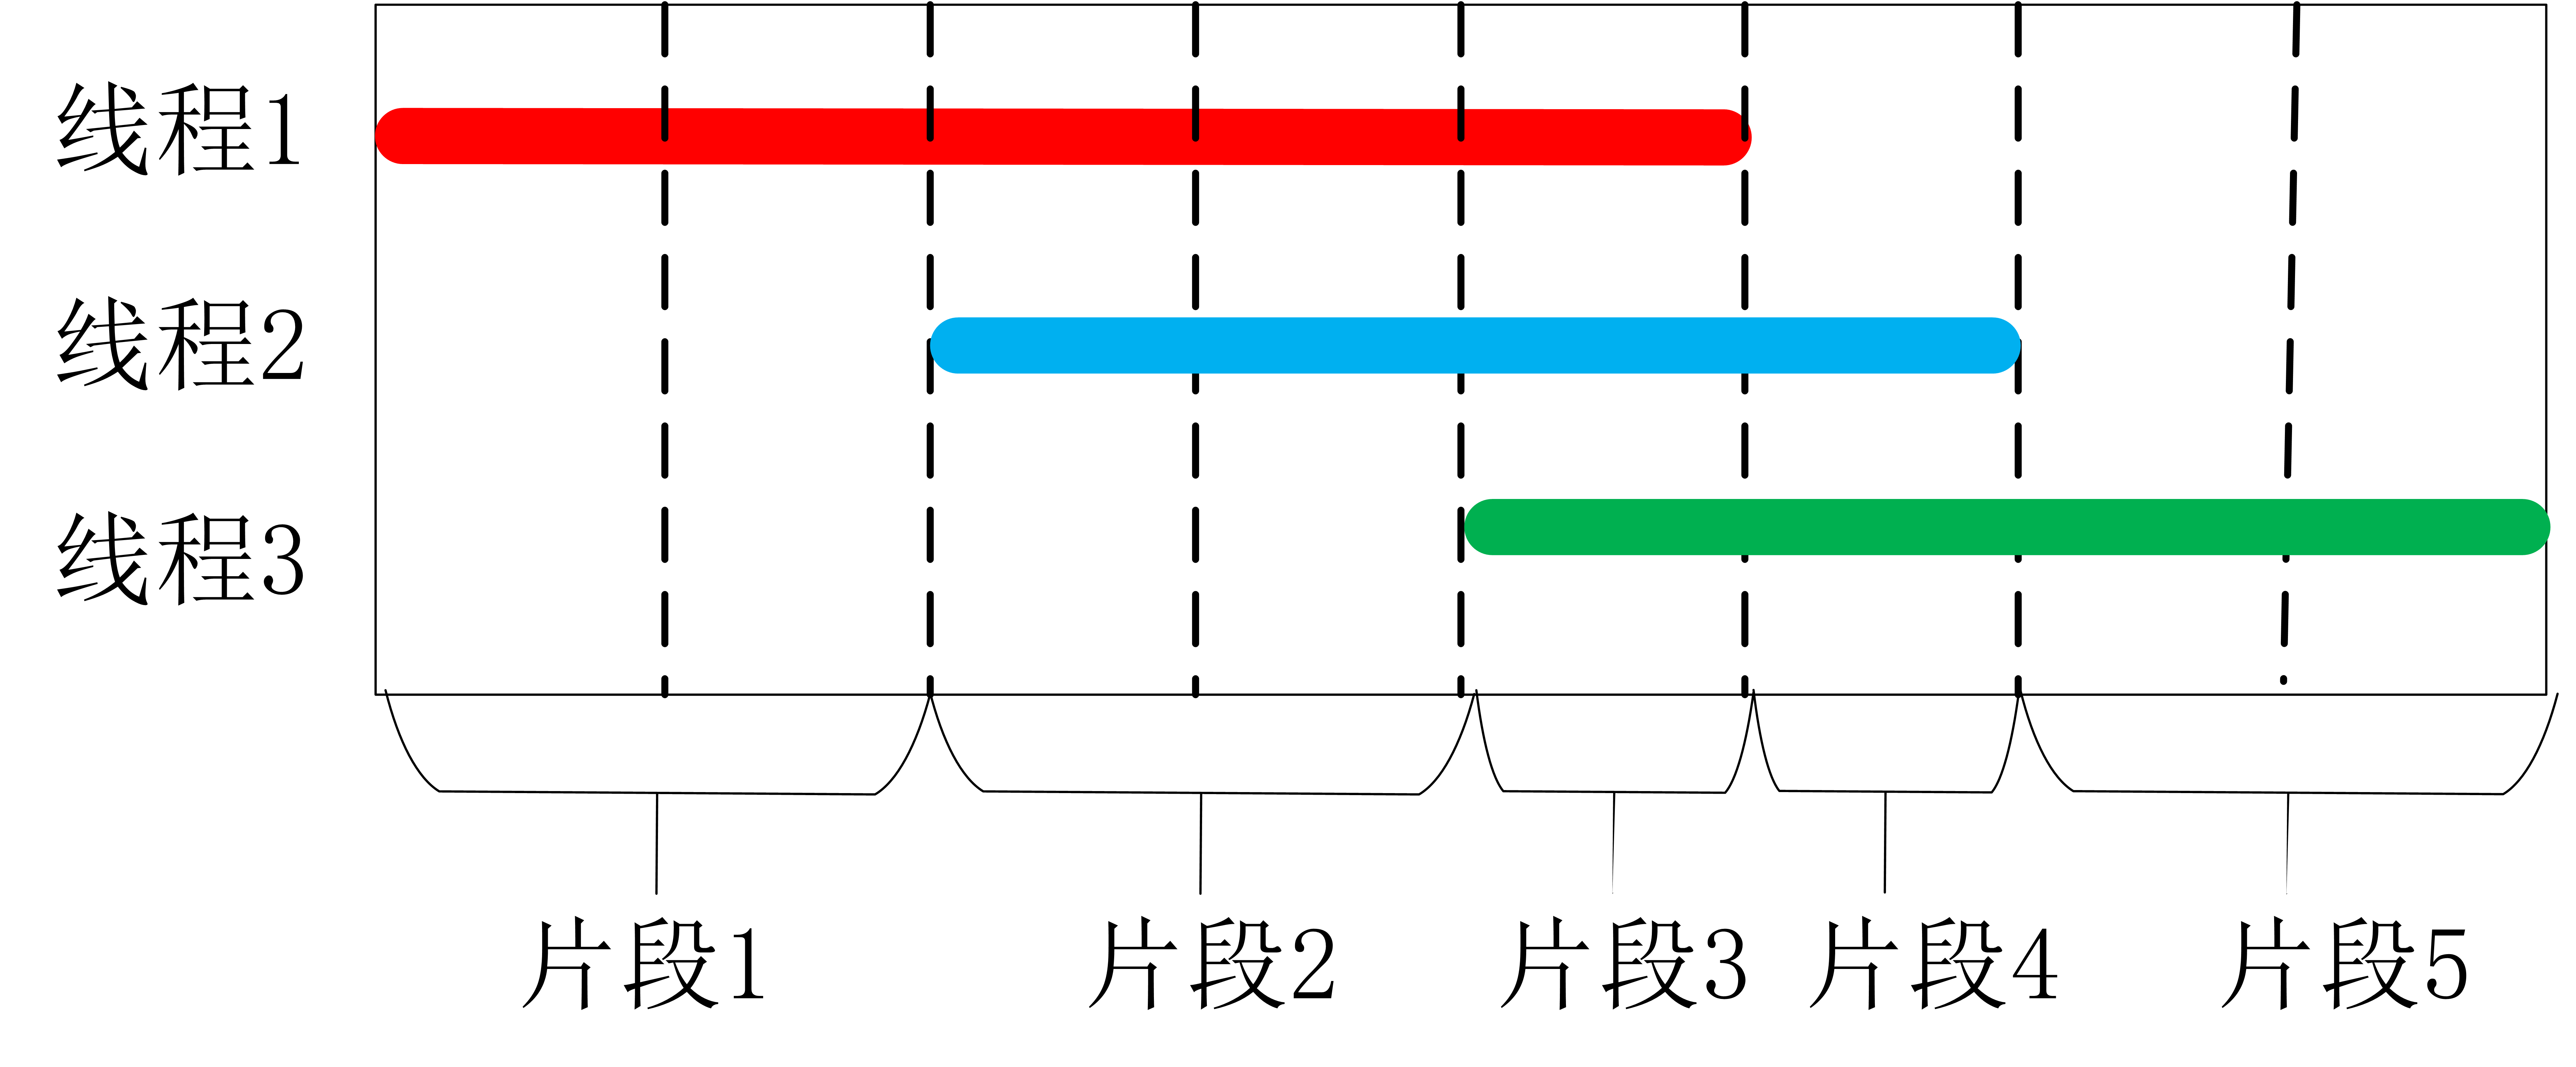
\includegraphics[width=0.8\linewidth]{figures/interval.png}
    \caption{缓存分段示意图}
    \label{fig:interval}
\end{figure}

分段过后,一个程序的分配区域可以被看成几个连续的缓存片段的组合。显然,无论在何种分配组合下,总的缓存片段数都会小于等于总的缓存路数。在每个缓存片段中,分配中包含这段的程序之间互相竞争,我们预测算法的核心就在于预测每个缓存片段的竞争结果。只要得到了每个缓存片段中各个程序的实际缓存占用,我们就可以汇总得到程序总的缓存占用,再通过MRC曲线就可以得到该程序的失效率。

在竞争中,缓存占用和失效数息息相关,竞争的深层原因实际上就是缓存失效淘汰了别的程序所占用的缓存块从而占为己有。失效数与缓存占用存在着一种负反馈的关系。失效数越多,往往意味着更多的缓存占用;反过来看,更多的缓存占用意味着更少的失效。在负反馈关系下,最后会达到一个稳定的状态,这个状态下的失效数和缓存占用都会稳定下来。假设程序的访存模式是恒定的,这个稳定状态就是程序运行时长期保持的状态,稳定状态时的缓存占用和失效率就是真实的缓存占用和失效率。CAPS预测模型的核心就是通过一个迭代算法求解这个稳定状态,算法伪代码如算法\ref{alg:pred}所示。

\begin{algorithm}
\caption{预测算法伪代码}
\label{alg:pred}
\begin{algorithmic}[1]
\renewcommand{\algorithmicforall}{\textbf{foreach}}
\renewcommand{\algorithmicrequire}{\textbf{Input:}}
\renewcommand{\algorithmicensure}{\textbf{Output:}}
\REQUIRE $MRC[i][]$ and $API[i]$ of each program $i$; a CAT scheme
\ENSURE $MissRate[i]$, $IPC[i]$ for each program $i$
\STATE Partition cache space to shared intervals based on allocations' starting and finishing points
\STATE Initialize $occupancy[i][j]$ for program $i$ in interval $j$ = (size of interval $j$) / (number of programs sharing the interval)
\WHILE {aggregate change of occupancies > threshold}
	\STATE {/* occupancy to miss rate */}
    \FORALL {program $i$}
    	\STATE $occ$ = $0$
    	\FORALL {interval $j$}
			\STATE $occ$ += $occupancy[i][j]$
        \ENDFOR
        \STATE $MissRate[i]$ = $MRC[i][occ]$
        \STATE $IPC[i]$ = $1 / (CPI_{base} + MissRate[i] * API[i] * MissPenalty)$
        \STATE $Miss[i]$ = $MissRate[i] * API[i] * IPC[i] * step$
    \ENDFOR
    \STATE {/* miss rate to occupancy */}
    \FORALL {interval $j$}
    	\STATE $TotalIntervalMiss$ = $0$
   		\FORALL {program $i$ in interval $j$}
        	\STATE $IntervalMiss[i][j]$ = $Miss[i] * IntervalSize[j] / AllocationSize[i]$
            \STATE $TotalIntervalMiss$ += $IntervalMiss[i][j]$ 
		\ENDFOR
        
        \FORALL {program $i$ in interval $j$}
        	\STATE $occupancy[i][j]$ =  $occupancy[i][j] + IntervalMiss[i][j] * (IntervalSize[j] - occupancy[i][j]) / IntervalSize[j] - (TotalIntervalMiss - IntervalMiss[i][j]) * occupancy[i][j] / IntervalSize[j]$
		\ENDFOR
    \ENDFOR
    \IF {$step$ > $minStep$}
    	\STATE $step$ = $step * StepReductionRatio$
    \ENDIF
\ENDWHILE

\STATE \textbf{return} $MissRate[]$, $IPC[]$

\end{algorithmic}
\end{algorithm}

每个程序的失效率曲线(MRC)和访存指令占比(API)是该预测算法的输入参数,该算法通过迭代过程得到稳定状态下的实际缓存占用。作为迭代的初始状态,我们首先需要给出一个初始占用。这个占用可以是随机的,并不影响最后的结果,但是会影响迭代收敛的速度。在CAPS的实现中,我们使用平均分配作为初始占用。在每次迭代的前半部分,我们根据当前的占用结果计算得到每个程序的失效率、失效数和IPC;在迭代的后半部分,我们根据当前的失效数和IPC推导出下一阶段的占用。直到缓存占用的变化程度小于一定的阈值,我们认为迭代收敛,此时的占用即是我们要求的稳定状态下的真实占用。

在介绍之前,我们引入了一个迭代步长参数$Step$来控制收敛过程。$Step$模拟在冷启动中每次迭代的步长,它也可以被看成公式\ref{eq:accesses}中的周期数。更大的步长通常意味着更快的收敛速度,但是同时也可能造成某次迭代越过了均衡点,导致迭代在均衡点两侧跳动从而无法收敛。另一方面,较小的步长可能会影响收敛速度,降低预测算法的效率。在CAPS中,我们选择了一个较大的初始$Step$,然后逐渐地降低它,每轮迭代降低5\%,直到设定的最低点。这样的话,我们可以在保证收敛到均衡点的同时提升了收敛速度。

首先我们来看迭代的前半部分,即通过当前的缓存占用来推导失效率、失效数和IPC。事实上,上一节的离线采样我们已经得到了每个程序的$MRC$,根据当前的缓存占用直接查阅MRC就可以得到失效率$MissRate$。失效数和IPC可以通过以下两个公式推导:

\begin{equation}
Misses = MissRate \times API \times IPC \times Step 
\label{eq:accesses}
\end{equation}

\begin{equation}
IPC = \frac{1}{CPI_{base} + API \times MissRate \times MissPenalty}
\label{eq:IPC}
\end{equation}

有了$MissRate$可以根据公式\ref{eq:accesses}计算得到失效数$Misses$。而$IPC$比较难以估计,因为很多因素都可以影响到IPC。这里,我们通过公式\ref{eq:IPC}来做一个近似估计。$CPI_{base}$和$MissPenalty$通过真实机器上的实验来估计。$CPI_{base}$通过一个失效率很低的测试程序来估计,而$MissPenalty$通过LLC的失效延迟来估计。   

注意,公式\ref{eq:accesses}得到的是该程序总的失效数。因为英特尔处理器使用了特殊的哈希函数来处理内存地址到缓存块的映射,可以近似地认为这种映射方式是充满了随机性的,所以缓存失效可以近似地被认为在分配区域内均匀分布。某个缓存片段中产生的失效占总体失效数的比例与片段大小占总的分配大小的比例是相同的。根据总的失效数和缓存片段大小占该程序分配区域的比例,就可以就可以得到每个缓存段的失效数。

我们再来看迭代的后半部分,即通过当前的失效数和IPC,来推导并更新缓存的占用情况。考虑到每个缓存片段的大小和竞争的程序都是不同的,对于每个缓存片段,我们分个击破。那么如何根据失效数和IPC来推导新的缓存占用呢?West等在一篇论文中介绍了一种双线程下缓存占用实时预测的方法\parencite{west2010online},该研究是通过硬件实时抓取到失效率来预测两个线程的缓存占用情况。虽然使用场景与我们的场景并不相同,但这个研究启发了我们建立了一个类似的定理用来计算多个程序的缓存占用。为了简化模型,我们假设所有程序都是单线程的,且在不同的核上执行。

\textbf{定理:}\emph{考虑一个容量为$C$的LLC,被$N$个并发程序所共享。每个程序目前分别占用了$C_1, C_2, ... , C_N$的缓存大小,并且在这一阶段分别产生了$M_1, M_2, ... , M_N$个失效。设$M$为失效数的总和,则对于程序$i$来说,它更新后的缓存占用为:$C_i' = C_i + \frac{C-C_i}{C} \cdot M_i - \frac{C_i}{C} \cdot (M-M_i)$.}

\textbf{证明:}首先,我们假设整个LLC空间已经被这$N$个程序充满。事实上,除了冷启动外,绝大多数时间LLC都是被充满的。充满状态下,每一次的失效都会淘汰一个缓存块。这时,如下公式成立:

\begin{equation}
C = \sum_{i=0}^{N} C_i
\label{eq:sumc}
\end{equation}

其次,我们假设每个缓存块都有均等的概率被替换。虽然在LRU策略下,这个假设通常是不正确的。失效的访存会替换掉最近最少被使用(LRU)的那个缓存块,这就意味着经常被访问的缓存块被替换的概率较小。然而,为了模型简洁性,我们仍然使用这一假设。事实上,这一假设不会给准确率带来很大影响\parencite{west2010online}。

当程序$i$发生了一个失效时,它淘汰掉的缓存块属于其他程序的概率为:$\frac{C-C_i}{C}$,这就相当于把缓存块从其他程序那里抢夺过来。程序$i$在单位时间内总共产生了$M_i$个失效,所以因为失效而抢夺过来的缓存块数量为:$\frac{C-C_i}{C} \cdot M_i $。在另一方面,其他程序的失效也可能从它这里抢夺一部分缓存块。一个缓存块属于程序$i$的概率为$\frac{C_i}{C}$,其他程序产生的失效数为$(M-M_i)$,所以其他程序从它这里抢夺的缓存块数量为:$\frac{C_i}{C} \cdot (M-M_i)$。在这个阶段过后,该程序占用的缓存块数量变动即为,抢夺来的缓存块减去被抢夺走的缓存块:

\begin{equation}
 \Delta C = \frac{C-C_i}{C} \cdot M_i - \frac{C_i}{C} \cdot (M-M_i)
 \label{eq:deltac}
\end{equation}

更新后的缓存占用为:

\begin{equation}
 C_i' = C_i + \frac{C-C_i}{C} \cdot M_i - \frac{C_i}{C} \cdot (M-M_i)
 \label{eq:occupancy}
\end{equation}

更新后的缓存占用仍然符合公式\ref{eq:sumc},所有$C_i'$之和仍然为$C$。在CAPS预测模型中,我们对于某个缓存片段,使用公式\ref{eq:occupancy}计算每轮迭代更新后的缓存占用,然后将所有缓存段的占用加总,就得到了该程序在当前迭代轮的总缓存占用。

此时就完成了一轮迭代,然后进入下一轮迭代的前半部分,根据更新后的缓存占用再来计算新的失效率、失效数和IPC。当缓存占用的变化率小于一定的阈值后,我们认为迭代已经收敛,即我们要求的稳定状态已经达到,CAPS预测模块会输出此时每个程序的失效率和IPC。

\section{分配优化} \label{sec:allocation}
% Copyright (c) 2014,2016 Casper Ti. Vector
% Public domain.

\subsection{算法综述}

本章节中,我们将介绍CAPS的优化算法。该优化算法基于上一章节的预测模型,可以针对一个优化目标,在较短时间内生成一个优化CAT分配方案。同时,该算法还支持不同的优化目标,我们在CAPS中实现了五个优化策略,在后文中会着重阐述。

缓存的优化问题可以被概括为一句话:给定一个优化目标,找到一个最优分配。但是在CAT技术下的优化问题将面临更大的挑战,之前的研究不用考虑部分重叠和分配位置,但CAT下的分配优化无法绕过这两点。相比于之前只考虑分配数额的优化问题,CAT优化问题的搜索空间更加庞大。之前的优化算法只需要决定每个线程需要被分配多少缓存空间,而CAT下需要决定每个分配是从哪到哪,而且还允许部分重叠。显然,搜索整个解空间显然是不现实的,搜索的时间和空间开销都是极其惊人的。可以证明,在这种情况下找到一个最优分配是一个NP-hard问题。

因此,我们的算法并不寻求一个全局绝对最优的分配方案,而只需要一个较优解。事实上,由于预测的准确率并不十分精确,所以一个全局上的绝对最优解并没有太大意义,反而在短时间内找到一个较优解有更大的意义。为此,我们从经典的模拟退火算法中吸取智慧,构建了一个基于“模拟退火”的优化算法。我们的实验表明该算法在任何优化目标下都能起到良好的效果,具体实验评估结果见第\ref{chap:evaluation}章。

\subsection{优化目标} \label{sec:opt_goals}

在介绍优化算法之前,我们先来讨论一下优化的目标。优化的目标是一个优化策略锚定的指标,是驱动一个优化算法的重要动力。一个优化指标是对系统的总体优化目标的一个量化,不同的指标侧重点也不同,总体来说可以被概括为三个方面:性能(Performance)、公平(Fairness)和服务质量(QoS)。当然,一个指标也可以兼顾两个方面,但同时兼顾三个方面是不现实的~\parencite{hsu2006communist}。优化策略的目标就是将锚定的指标最小化或最大化,同时该指标也用来在实验中评估策略的有效性。

前人的研究中提出了许多指标来抽象多个并发程序的整体效能。这些指标大多依赖于IPC和失效率这两个参数,这也是CAPS预测模型会输出这两个参数的原因。我们希望我们的优化策略具有灵活性,可以很容易适应多个指标,而不用对不同的指标设计截然不同的策略。事实上,因为预测模型预测出了失效率和IPC,只要是基于这两个参数的指标,我们的优化策略都可以直接适配。在本文中,我们选择实现了五个指标作为参考。这五个指标涵盖了各种场合下的优化需求,包括上述所说的性能、公平和服务质量这三个方面。

我们在CAPS中实现的五个指标为:

\begin{itemize}

\item \textbf{平均失效数(Average MPKI):}平均失效数Average MPKI代表平均每1000条指令的失效数(Misses Per 1000 Instructions, MPKI)。MPKI是系统评估中的常用指标之一,平均失效数代表所有并发程序的平均MPKI,它可以体现出该并发系统的缓存利用效率。较小的平均失效数意味着较高的缓存利用效率,所以针对该指标的优化策略目的就是让平均MPKI尽可能的小。另一方面,LLC缓存失效就意味着该访存指令需要访问内存,所以最小化MPKI也意味着降低内存总线的竞争。在下述公式中,我们定义$MissRate_i$为程序$i$在和别的程序并发执行时的失效率,$APKI_i$是程序$i$每1000条指令的访存指令数。Average MPKI是一个越小越好的指标。

\begin{equation}
AverageMPKI = \sum ( MissRate_i \times APKI_i ) / \#program
\label{eq:mn}
\end{equation}
	
\item \textbf{吞吐量(Throughput):}吞吐量Throughput被定义为所有程序的IPC之和,这也是一个被广泛使用的指标。针对该指标的策略力求让系统整体的IPC吞吐量最大化。它把所有并发程序看成一个整体,使得整个系统的执行效率最高。但是,该指标可能会对一些本身IPC就比较低的程序不太公平,因为降低它们的IPC并不会对整体系统的IPC之和产生非常大的影响。在下述公式中,我们定义$IPC_i$为程序$i$在并发负载中的IPC。Throughput是一个越大越好的指标。

\begin{equation}
	Throughput = \sum IPC_i
	\label{eq:IPCsum}
\end{equation}

\item \textbf{平均效率下降(Average Slowdown):}平均效率下降Average Slowdown代表着在平均情况下,程序的在共享LLC与独占LLC的执行时间之比。因为相比于一个程序独占LLC,共享的情况下或多或少都会受到一定的性能损失,所以每个程序的Slowdown一定是大于1的,平均Slowdown自然也大于1。我们定义对于程序$i$来说,它的Slowdown为$SingleIPC_i/IPC_i$,这里$SingleIPC_i$指的是当它单独运行使用全部LLC时每周期执行的指令数(IPC),$IPC_i$是在多程序并发负载中的IPC。平均Slowdown的概念与前人研究中多次提到的另一个指标,加权效率提升(Weighted Speedup),有很大相似之处~\parencite{snavely2000symbiotic,qureshi2006utility}。Weighted Speedup把并发执行的程序看成一个整体,Speedup是Slowdown的倒数,用来加总的Speedup而不是平均意义上的Slowdown,可以概括系统作为一个整体因为并发带来的效率提升。但是我们认为,每个并发的程序还可以看作独立的个体,每个程序执行各自不同的任务,这样的话针对单个程序的Slowdown可以更好地反映出程序的执行效率。相比于独占LLC,共享情况下的性能必定会下降,所以一定会引起每个程序或多或少的效率下降,换句话说每个并发程序的Slowdown一定大于1。我们把所有程序的Slowdown做算术平均,就可以得到该并发负载因为共享LLC导致的整体性能下降。Average Slowdown是一个越低越好的指标。

\begin{equation}
	AverageSlowdown = \sum\frac{SingleIPC_i}{IPC_i} / \#program
\end{equation}

\item \textbf{公平效率下降(Fair Slowdown):}公平效率下降指标Fair Slowdown兼顾了整体性能和公平性。这个指标借鉴了多个前人的研究经验~\parencite{luo2001balancing, chang2014cooperative}。如果只考虑公平性而无视性能是没有意义的,因为大家效率都很差的话,即使再公平也意义不大。我希望通过指标能在提升性能的基础上兼顾公平。与上一个指标Average Slowdown不同之处在于,本指标被定义为各个程序Slowdown的调和平均。调和平均鼓励大家的差距尽量小,鼓励各个程序的Slowdown得到均匀地改善。Fair Slowdown是一个越小越好的指标。

\begin{equation}
	FairSlowdown = \#program / {\sum\frac{IPC_i}{SingleIPC_i}}
\end{equation}

\item \textbf{最大效率下降(Maximum Slowdown):}最大效率下降Maximum Slowdown指的是所有并发程序中Slowdown最大的那一个,它兼顾了性能与服务质量(QoS)。事实上,QoS是比较难以被量化的,因为判断哪些程序优先级较高,哪些程序优先级较低本身就比较主观。在本文中,我们不讨论程序间优先级不同这一主观因素,我们把并发负载看成一个木桶,把QoS定义成木桶中最短的那块短板,也就是Slowdown最高的那个程序。这种表达QoS的方法也被之前的研究者所使用~\parencite{manikantan2012probabilistic}。Maximum Slowdown是一个越小越好的指标。

\begin{equation}
MaxSlowdown=\max(\frac{SingleIPC_i}{IPC_i})
\label{eq:qos}
\end{equation}

\end{itemize}

\subsection{优化算法}

在本节中,我们将介绍CAPS生成优化分配的算法。一个CAT分配组合包含对每一个核/线程的分配所构成的集合,一个分配是LLC中任意一段连续的路。我们的目标是找到一个优化分配,使得给定的优化指标最大或最小化。之前研究面对的分配问题只需要决定分配的数量,而CAT下由于要求分配是连续的且允许部分重叠,所以分配的位置也需要被考虑进去。

CAT下的优化算法主要存在两点挑战:

首先,搜索空间随着核数增加而呈指数级增长,当核数较多时解空间会变得极其巨大。举例来说,对于一个20路的LLC,一共有210(1+2+3+..+20)种CLOS,或者说是可能的分配情况。对于一个$N$核的工作负载,$N$个程序并发执行,那么一共可能的CAT分配数为$210^N$。在4核情况下,解空间的规模就已经达到了1,944,810,000,全部搜索一遍显然是不太现实的,甚至搜索一小部分都要耗费大量的时间。

其次,之前的优化方案都不能适用于CAT。为了避免搜索的时间消耗,之前的解决方案多是通过启发式算法来找到优化分配,例如贪心算法~\parencite{suh2004dynamic}、前瞻算法(Lookahead Algorithm)~\parencite{qureshi2006utility}等。但这些解决方案都有一个隐含的假设,就是一个缓存路只能分配给一个核,并不能被两个或多个核所共用。这个假设在它们的分配技术下是成立的,然而在CAT下并不成立。所以这些解决方案都不能直接套用在CAT上。

因此,我们需要一个全新的算法来解决CAT下的分配优化问题。我们从经典算法中吸取经验,设计了一个基于模拟退火(Simulated Annealing)的算法,它可以针对任意优化目标生成一个优化分配方案。模拟退火算法是一个随机化算法,它可以在一个庞大的解空间中找到一个全局近似最优解~\parencite{aarts1988simulated,hwang1988simulated}。该算法适合被应用在搜索空间较大并且离散的情况下,CAT优化问题的搜索空间正符合这一特征。同时,模拟退火适合在有限时间内找到一个近似最优解,而不是全局最优解。在CAT优化问题中,短时间内找一个优化解确实比花费大量时间找到一个全局绝对最优解有更大的意义。综上,模拟退火算法是CAT优化问题的一个有效的解决思路。

\begin{algorithm}
\caption{优化算法伪代码}
\label{alg:opt}
\begin{algorithmic}[1]
\renewcommand{\algorithmicforall}{\textbf{foreach}}
\renewcommand{\algorithmicrequire}{\textbf{Input:}}
\renewcommand{\algorithmicensure}{\textbf{Output:}}
\REQUIRE concurrent programs and a metric function
\ENSURE a near-optimal CAT scheme
\STATE Profile $MRC[i][]$ and $API[i]$ for each program $i$
\STATE Initialize temperature $T$ and a random allocation $scheme$
\STATE $IPC[]$,$MissRate[]$ = Predict($scheme$)
\STATE $metric$ = CalculateMetric($IPC[]$,$MissRate[]$)
\WHILE {$T < T_{min}$}
	\STATE $scheme'$ = RandomNeighbor($scheme$)
    \STATE $IPC[]$,$MissRate[]$ = Predict($scheme'$)
    \STATE $metric'$ = CalculateMetric($IPC[]$,$MissRate[]$)
    \IF {$metric'$ is better than current $bestMetric$}
    	\STATE $bestMetric$ = $metric'$ 
        \STATE $bestScheme$ = $scheme'$
    \ENDIF
    \IF {$metric$ is lower-is-better}
    	\STATE {$diff$ = $metric'$ - $metric$}
    \ELSE
    	\STATE {$diff$ = $metric$ - $metric'$}
    \ENDIF
    \IF {$diff$ < 0 \OR $\exp(-diff / (k * T)) \leq Random(0,1)$ }
    	\STATE {$metric$ = $metric'$}
        \STATE {$scheme$ = $scheme'$}
    \ENDIF
    \STATE $T$ = $T$ * $TemperatureReductionRatio$
\ENDWHILE
\STATE \textbf{return} $bestScheme$

\end{algorithmic}
\end{algorithm}

CAPS的优化算法伪代码如算法\ref{alg:opt}所示。算法过程可以被看作在CAT分配方案的解空间中的随机游走。我们随机生成的一个CAT分配组合作为游走的起始节点。每一轮,本算法从两个决策中选择一个执行:停留在当前节点,或者走到一个相邻节点。我们认为两个分配组合是相邻的,当且仅当这个两个分配组合中只在某一个核的分配上相差一个缓存路的配额。

不同于爬山算法(Hill Climbing Algorithm)每次都往更好的方向走,模拟退火算法有可能会朝更坏的方向走。爬山算法的劣势在于会陷入局部最优解,只能找到最近的山顶而不是全局的山顶。另一方面,模拟退火算法由于允许往更坏的节点走,就会跳出局部的小山,从而找到别处更高的山峰。

我们的算法从随机生成的初始分配方案出发,每次会从当前节点的分配方案中,随机选一个核的分配,然后随机从该分配中的左边或右边选择一边,再随机决定加一个路或减一个路,这样来随机生成一个相邻的分配方案,作为下一步的潜在节点进行考察。值得一提的是,随机生成的邻居分配方案必须是合法的,换句话说说该方案内的每个核的配额都必须大于等于0且小于等于总的路数。

考察的方法,就是将该分配方案输入到上一章介绍的预测模型中,得到每个程序的失效率和IPC参数。这两个参数用来计算得到优化指标的值,这里的优化指标具备灵活性,只要是基于失效率和IPC的指标都可以被该算法所接受。比如说,对于IPC吞吐量这个指标,我们就将预测得到的每个程序的IPC相加。

得到邻居分配方案的指标数值后,我们将该指标与当前节点的指标相比较,看是更好了还是更坏了。如果邻居节点更好,算法将会无条件走到这个节点上。如果邻居更差,那么算法还是有一定的概率会走向这个节点。这个概率与当前的“温度”有关,这也是模拟退火算法的精华之处。简而言之,在温度较高时,有更大的概率走向更差的节点,而在温度较低时,走向较差节点的概率更小。温度正是模拟了金属退火的降温冷却过程。初始温度较高,走动随机性更强,而随着温度逐渐降低,走动会越来越偏向于往更优的方向走。这种游走方式可以有效地防止陷入到局部最优解中。

具体来说,算法中允许走到更差节点的概率与选定的指标是越小越优还是越大越优有关。对于越小越优的指标,接受一个较差移动的概率为$\exp(-\Delta e / (kT))$;而对于一个越大越优的指标,概率为$\exp(\Delta e / (kT))$。这里的$\Delta e$指的是待考察的邻居节点与当前节点的指标差额,$k$是一个可以控制的常量参数,$T$是当前的温度。通常,温度$T$的变化会由一个单调递减函数决定。

常量参数$k$的选取,以及$T$的变化函数,对算法的执行时间和有效性都有较大影响。越高的初始温度,越慢的下降速度,越大的$k$,会带来越大的随机性,会搜索到更多的节点,所以也更可能搜索到更优的结果。但同时,时间的开销也会增加。为了平衡算法的效率和效果,我们通过大量的实验选择了合适的参数和温度变化函数,使得算法可以在短时间内找到一个比较好的解。具体的实验评估结果会在下一章给出。
	% Copyright (c) 2014,2016 Casper Ti. Vector
% Public domain.

\chapter{实验评估} \label{chap:evaluation}

\section{实验方法}

我们的实验测试机器采用了英特尔至强Xeon E5-2699 v4处理器。该处理器支持CAT技术,拥有22个处理器核心,它们共享一个20路、大小为55MB的L3缓存,每一个缓存路的容量为2816KB。处理器一共包含16个CLOS,也就是说最多支持16种不同的分配。此外,每个核有一个32KB的私有L1指令缓存、一个32KB的私有L1数据缓存和一个256KB的私有L2缓存。因为多级采用了包含式设计,所以在CAPS中我们并没有考虑私有的L1和L2缓存。该实验环境的内存带宽为76.8GB/s,同时拥有64GB的内存,所以内存竞争的干扰因素较小。我们把测试程序封装到Docker中,每个Docker中运行一个不同的测试程序,并把各个Docker绑在不同的核上。我们通过一个英特尔提供的开源工具来执行CAT分配~\parencite{pqos}。因为不同的程序执行的时间长短也不一样,运行结束的时间点也会不同,在测试时,我们会让早结束的程序反复执行,直到最慢的程序执行完毕。在程序实时运行的同时,一些关键参数,比如运行时IPC、LLC失效数等等会通过硬件计数器(Performance Counter)统计收集,并且真实的缓存大小占用也通过会缓存监控技术(CMT)进行采集。

我们从SPEC CPU2006中选择了20个测试程序作为我们的评估对象,如表\ref{tab:benchmarks}所列。从中我们选择4到15个不同的程序组成一个并发执行的工作负载。虽然我们也想尝试测试更大的并发度,但是由于目前最高端的处理器只支持16个CLOS,同时一个默认的CLOS需要留给操作系统等其他程序,所以目前最大支持的并发度就是15。

对于每个程序,我们采用第\ref{sec:prediction_sample}节介绍的方法进行离线采样分析,得到每个程序的失效率曲线和访存频率,这两个特征会被预测模型所用到。为了了解多程序工作负载中各个程序的的特性,我们进一步将这20个测试程序分成了三个类别,如表\ref{tab:benchmarks}所示。这种分类方式和前人所提倡的类似~\parencite{lin2008gaining}。分类依据两个维度来考察每个程序:敏感度和污染度。敏感程度代表程序从缓存中的收益,一个敏感型程序会从较大的缓存占用获得较大收益,反之如果缓存占用较小会收到较大损害;而一个缓存不敏感的程序无论分配的缓存是大是小都不会受到太大影响。这里我们用缓存分配从6MB下降到1MB引起的程序运行效率的下降(Slowdown)来量化程序的敏感程度。由于CAT分配下一个路的大小动辄就几MB,所以Slowdown无法通过实测来得到。这里我们通过失效率曲线来估计程序的Slowdown。污染度主要指的是在竞争中该程序所能抢占的缓存多少,抢占的越多,别的程序得到的就越小,说明污染程度越重。污染度主要跟程序的访存频率相关,一般访存指令越多污染程度就越高。通常情况下,缓存敏感的程序因为有大量的访存指令,所以会占据较多缓存。但反过来并不成立,污染度较高的程序并不一定都是缓存敏感的。

我们把Slowdown大于10\%的归位A类。这一类程序对缓存敏感,同时它们通常也有较大的缓存需求,在竞争中会占用较多缓存资源,A类测试程序一共有9个,剩下11个程序根据它们的访存指令占比进一步划分为B类和C类。Slowdown小于等于10\%且每1000条指令的L3访存数大于5的程序被归位B类,这一类程序是不敏感但污染度较高的程序。B类程序有5个,它们会侵占大量的缓存然而并不会从中受益很多。最后,剩下的6个程序被归位C类,它们的Slowdown小于10\%,并且每1000条指令造成的L3访问也小于5,这一类程序属于既不敏感也不污染。多程序工作负载中A类、B类和C类程序的比例可能会对优化效果有影响,为了模拟各种情形,我们在实验中采用了不同的配比。

\begin{table}[htbp]
\caption{Benchmark classification}
\label{tab:benchmarks}
\centering
\begin{tabularx} {1\textwidth}{|l|l|l|X| } 
 \hline
 Type & Slowdown & APKI & Benchmarks \\
 \hline
 A & $> 10\%$ & $> 5$ & 401.bzip2 403.gcc 429.mcf 436.cactus 465.tonto 470.lbm 471.omnetpp 473.astar 482.sphinx\\ 
 \hline
 B & $\leq 10\%$ & $> 5$ & 410.bwaves 434.zeusmp 437.leslie3d 459.GemsFDTD 462.libquantum\\ 
 \hline
 C & $\leq 10\%$ & $\leq 5$ & 433.milc 445.gobmk 453.povray 456.hmmer 458.sjeng 464.h264ref\\
 \hline 
\end{tabularx}
\end{table}

正如在第\ref{sec:opt_goals}节所介绍的,我们选择并实现了5种优化策略,分别针对5种指标:平均失效数(Average MPKI)、吞吐量(Throughput)、平均效率下降(Average slowdown)、公平效率下降(Fair slowdown)和最大效率下降(Maximum slowdown)。前3个主要针对系统的综合性能,Fair slowdown兼顾了公平性和性能,而Maximum slowdown表示了QoS和性能。因为除了CAPS以外,目前并没有一个可以在真机上运行的优化框架可以做比较,所以我们实验只和完全竞争,以及无重叠分配方案做了比较。完全竞争就是传统意义上自由共享的LLC,也可以被认为所有分配都包含整个LLC且完全重叠。不重叠方案是前人研究普遍采用的分配方式,各个分配之间无重叠无共享。我们通过检索所有可能的无重叠方案,分别输入到CAPS预测模型中进行预测,然后找到一个最优的无重叠方案。因为重叠不存在,所以CAPS预测模型无需迭代,只要经过一次计算就可以得到预测结果。

我们对75个不同的工作负载进行实验,负载中包含的测试程序数从4个到15个不等。在下一节的实验结果中,我们在这5种优化目标下,分别对比了CAPS部分重叠方案、无重叠方案和完全重叠的自由竞争。

\section{实验结果}

因为预测模型是优化算法的基础,它的准确率对优化效果有重要影响。在我们的所有实验中,CAPS预测模型对失效率预测的平均准确率高达90.5\%,对IPC的预测平均准确率高达80.1\%,单次的预测时间平均为0.01秒。所以该预测模型无论从准确率还是开销上,都可以被接受。

\begin{figure}[htbp]
\centering
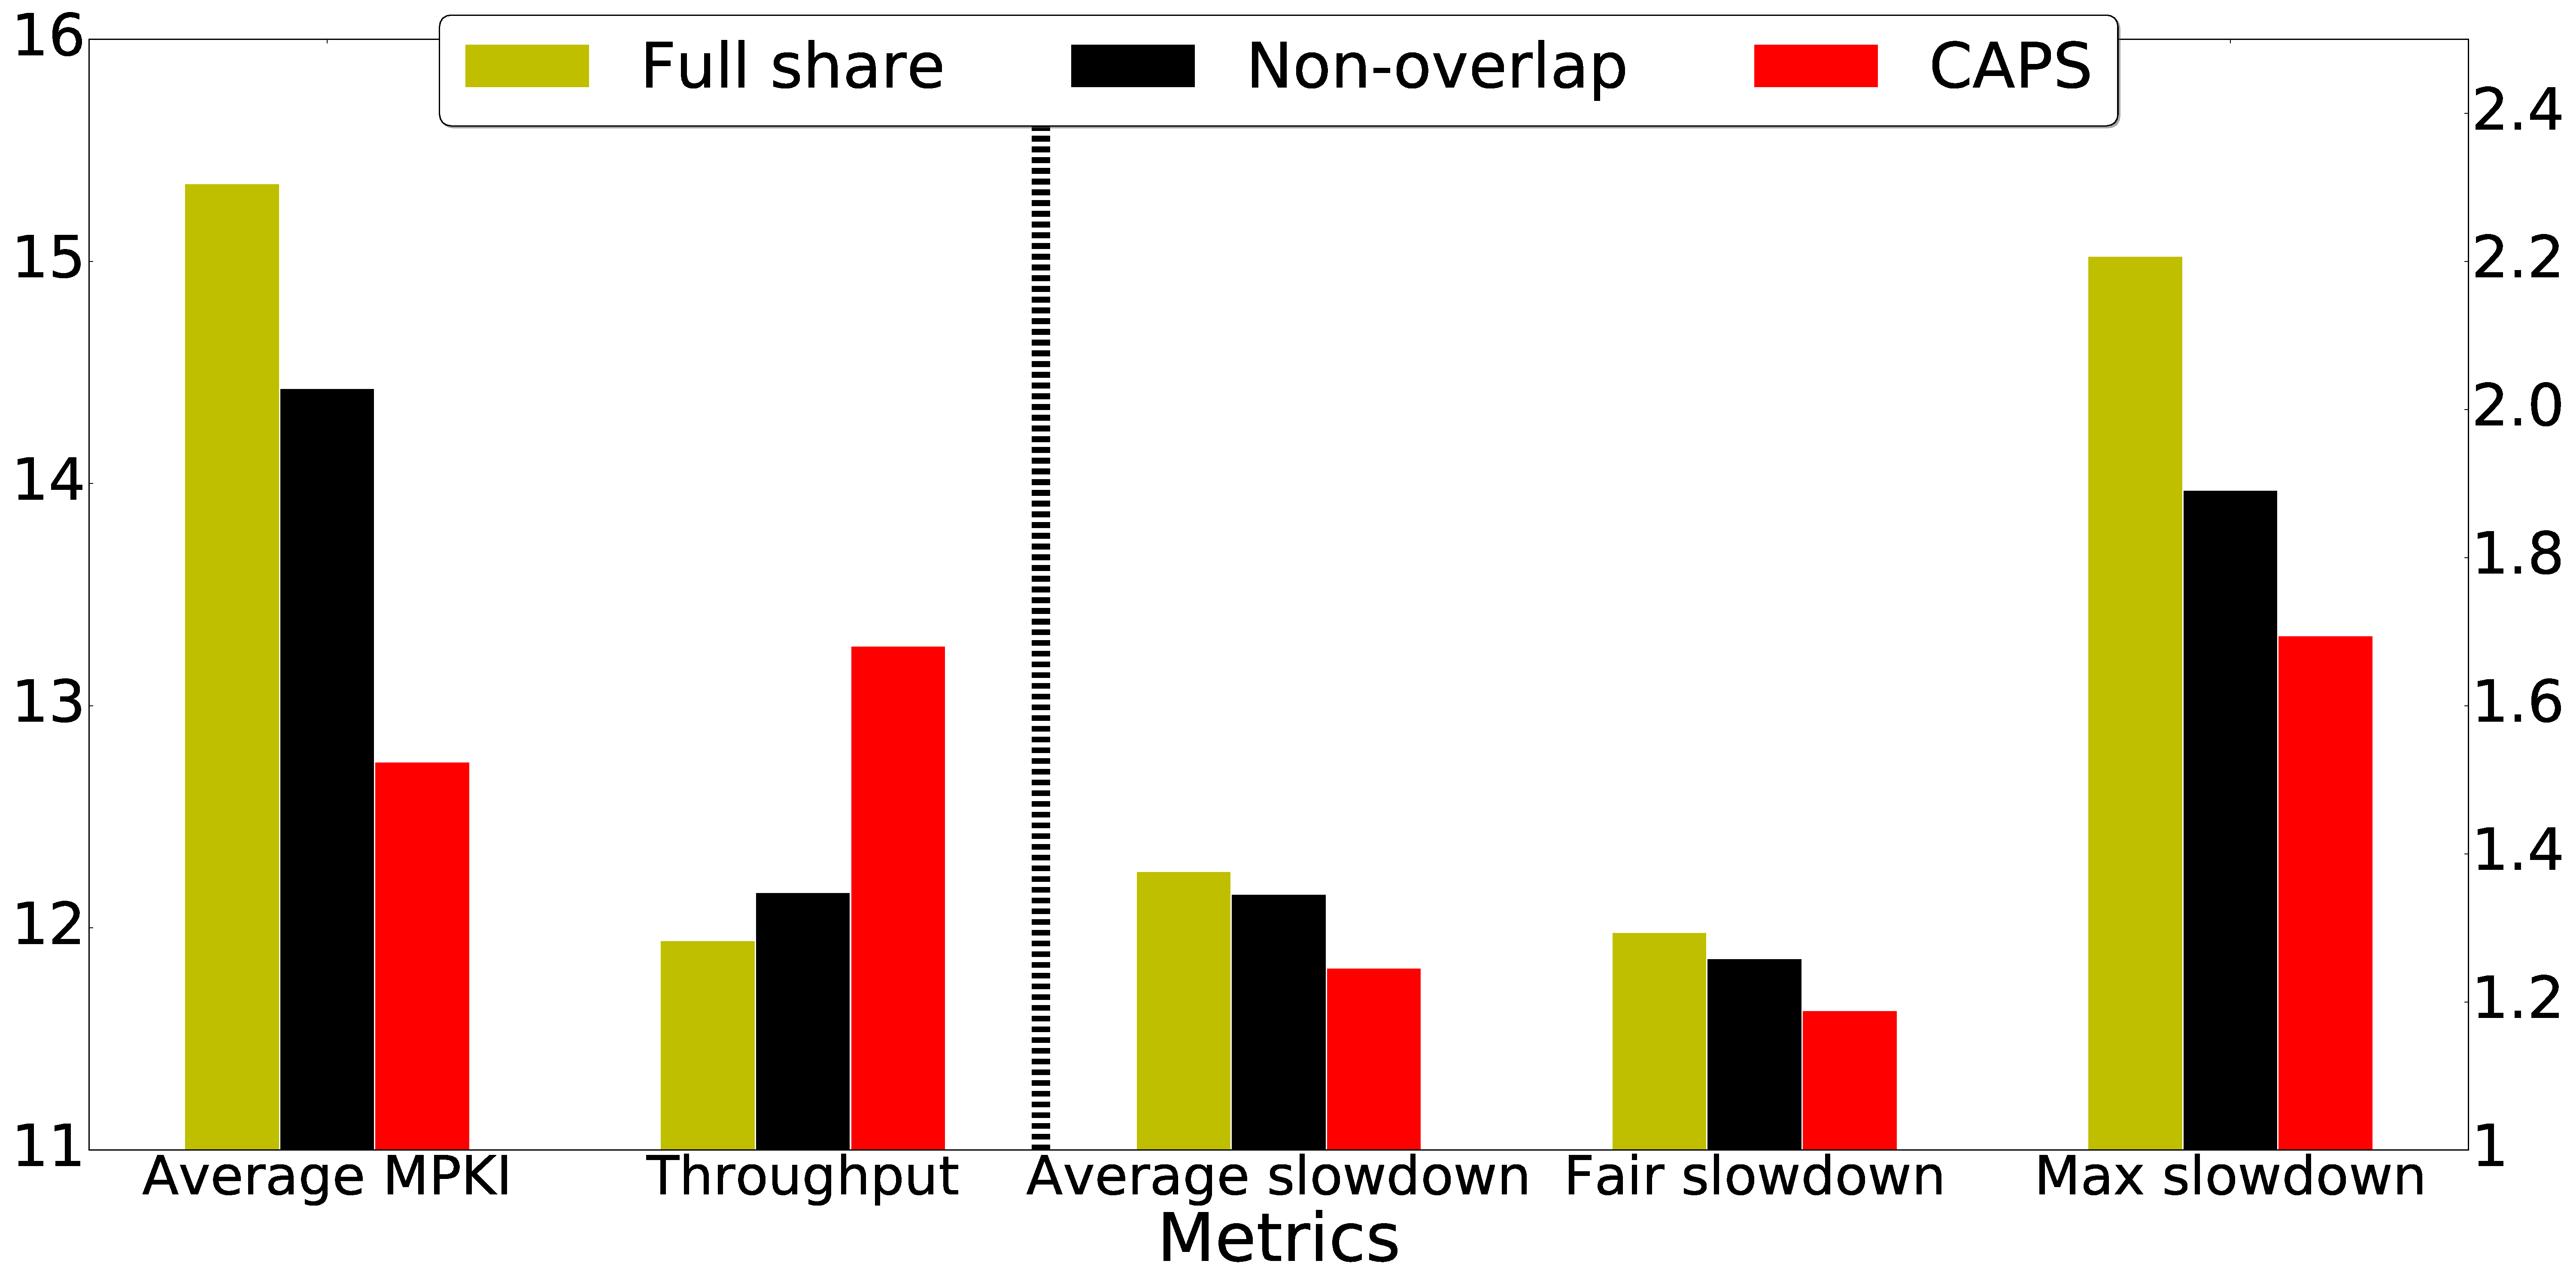
\includegraphics[width=0.9\columnwidth]{figures/avg_analysis.pdf}
\caption{完全重叠、不重叠与CAPS部分重叠方案的平均性能对比}
\label{fig:avg_an}
\end{figure} 

我们实现了5种优化目标。Average MPKI、Average slowdown、Fair slowdown和Maximum slowdown是越小越好的指标,而Throughput是越大越好的指标。对于每一个指标,CAPS会输出一个部分重叠的优化分配方案。我们将这个方案在真机上运行,将硬件计数器测量到的参数计算成指标值,与不重叠方案、完全重叠方案进行比较。我们一共测试了75种工作负载:4、6、8、12和15个并发程序的各10种,10个程序的25种。测试的平均结果如图\ref{fig:avg_an}所示。

\begin{itemize}
    \item 对于Average MPKI, CAPS相比于完全竞争在平均情况下可以减少16.96\%的失效数,最好情况下可以减少高达23.1\%。
    \item 对于Throughput,CAPS相比于完全竞争可以平均提升11.11\%,最好情况下可以提升31.3\%。
    \item 对于Average slowdown,CAPS平均可以缓解8.16\%,最好情况下达11.18\%。
    \item 对于Fair slowdown,CAPS平均可以优化8.17\%,最好情况下13.2\%。
    \item 对于Maximum slowdown,CAPS平均可以优化23.24\%,最好情况下33.42\%。
\end{itemize}

通常情况下,在核数/线程数较多时,在缓存敏感和污染程序较多时,CAPS可以提供更好的优化效果。在一共375次比较中(75个工作负载 * 5个指标),CAPS在354中胜出,比完全共享和不重叠方案中最好的那个还要好。CAPS的平均需要20秒左右来生成一个优化方案,这个时间并不包括对程序进行离线采样分析的过程。虽然对于一个离线优化方案,时间开销并不重要,但我们希望在未来可以把CAPS应用的在线实时优化上。对于在线优化的需求,我们可以通过降低算法\ref{alg:opt}的初始温度以及提升降温速度来进一步提升算法那效率。


\section{不同核数的评估分析}

在图\ref{fig:core_count}中,我们比较了在不同核数/线程数的情况下CAPS的优化效果与完全竞争和不重叠分配方案的对比。我们对比了4核、6核、8核、10核、12核以及15核的情况,对于$N$核的情况,我们选取$N$个不同的测试程序,绑在不同的核上同时执行,这样组成一个$N$核的工作负载。对于每一个核数,我们选取10到25种不同的工作负载,这些负载涵盖了不同的A类程序、B类程序和C类程序比例。平均测试结果见图\ref{fig:core_count}。

\begin{figure}[htbp] 
    \centering
    \begin{subfigure}[b]{0.5\linewidth}
        \centering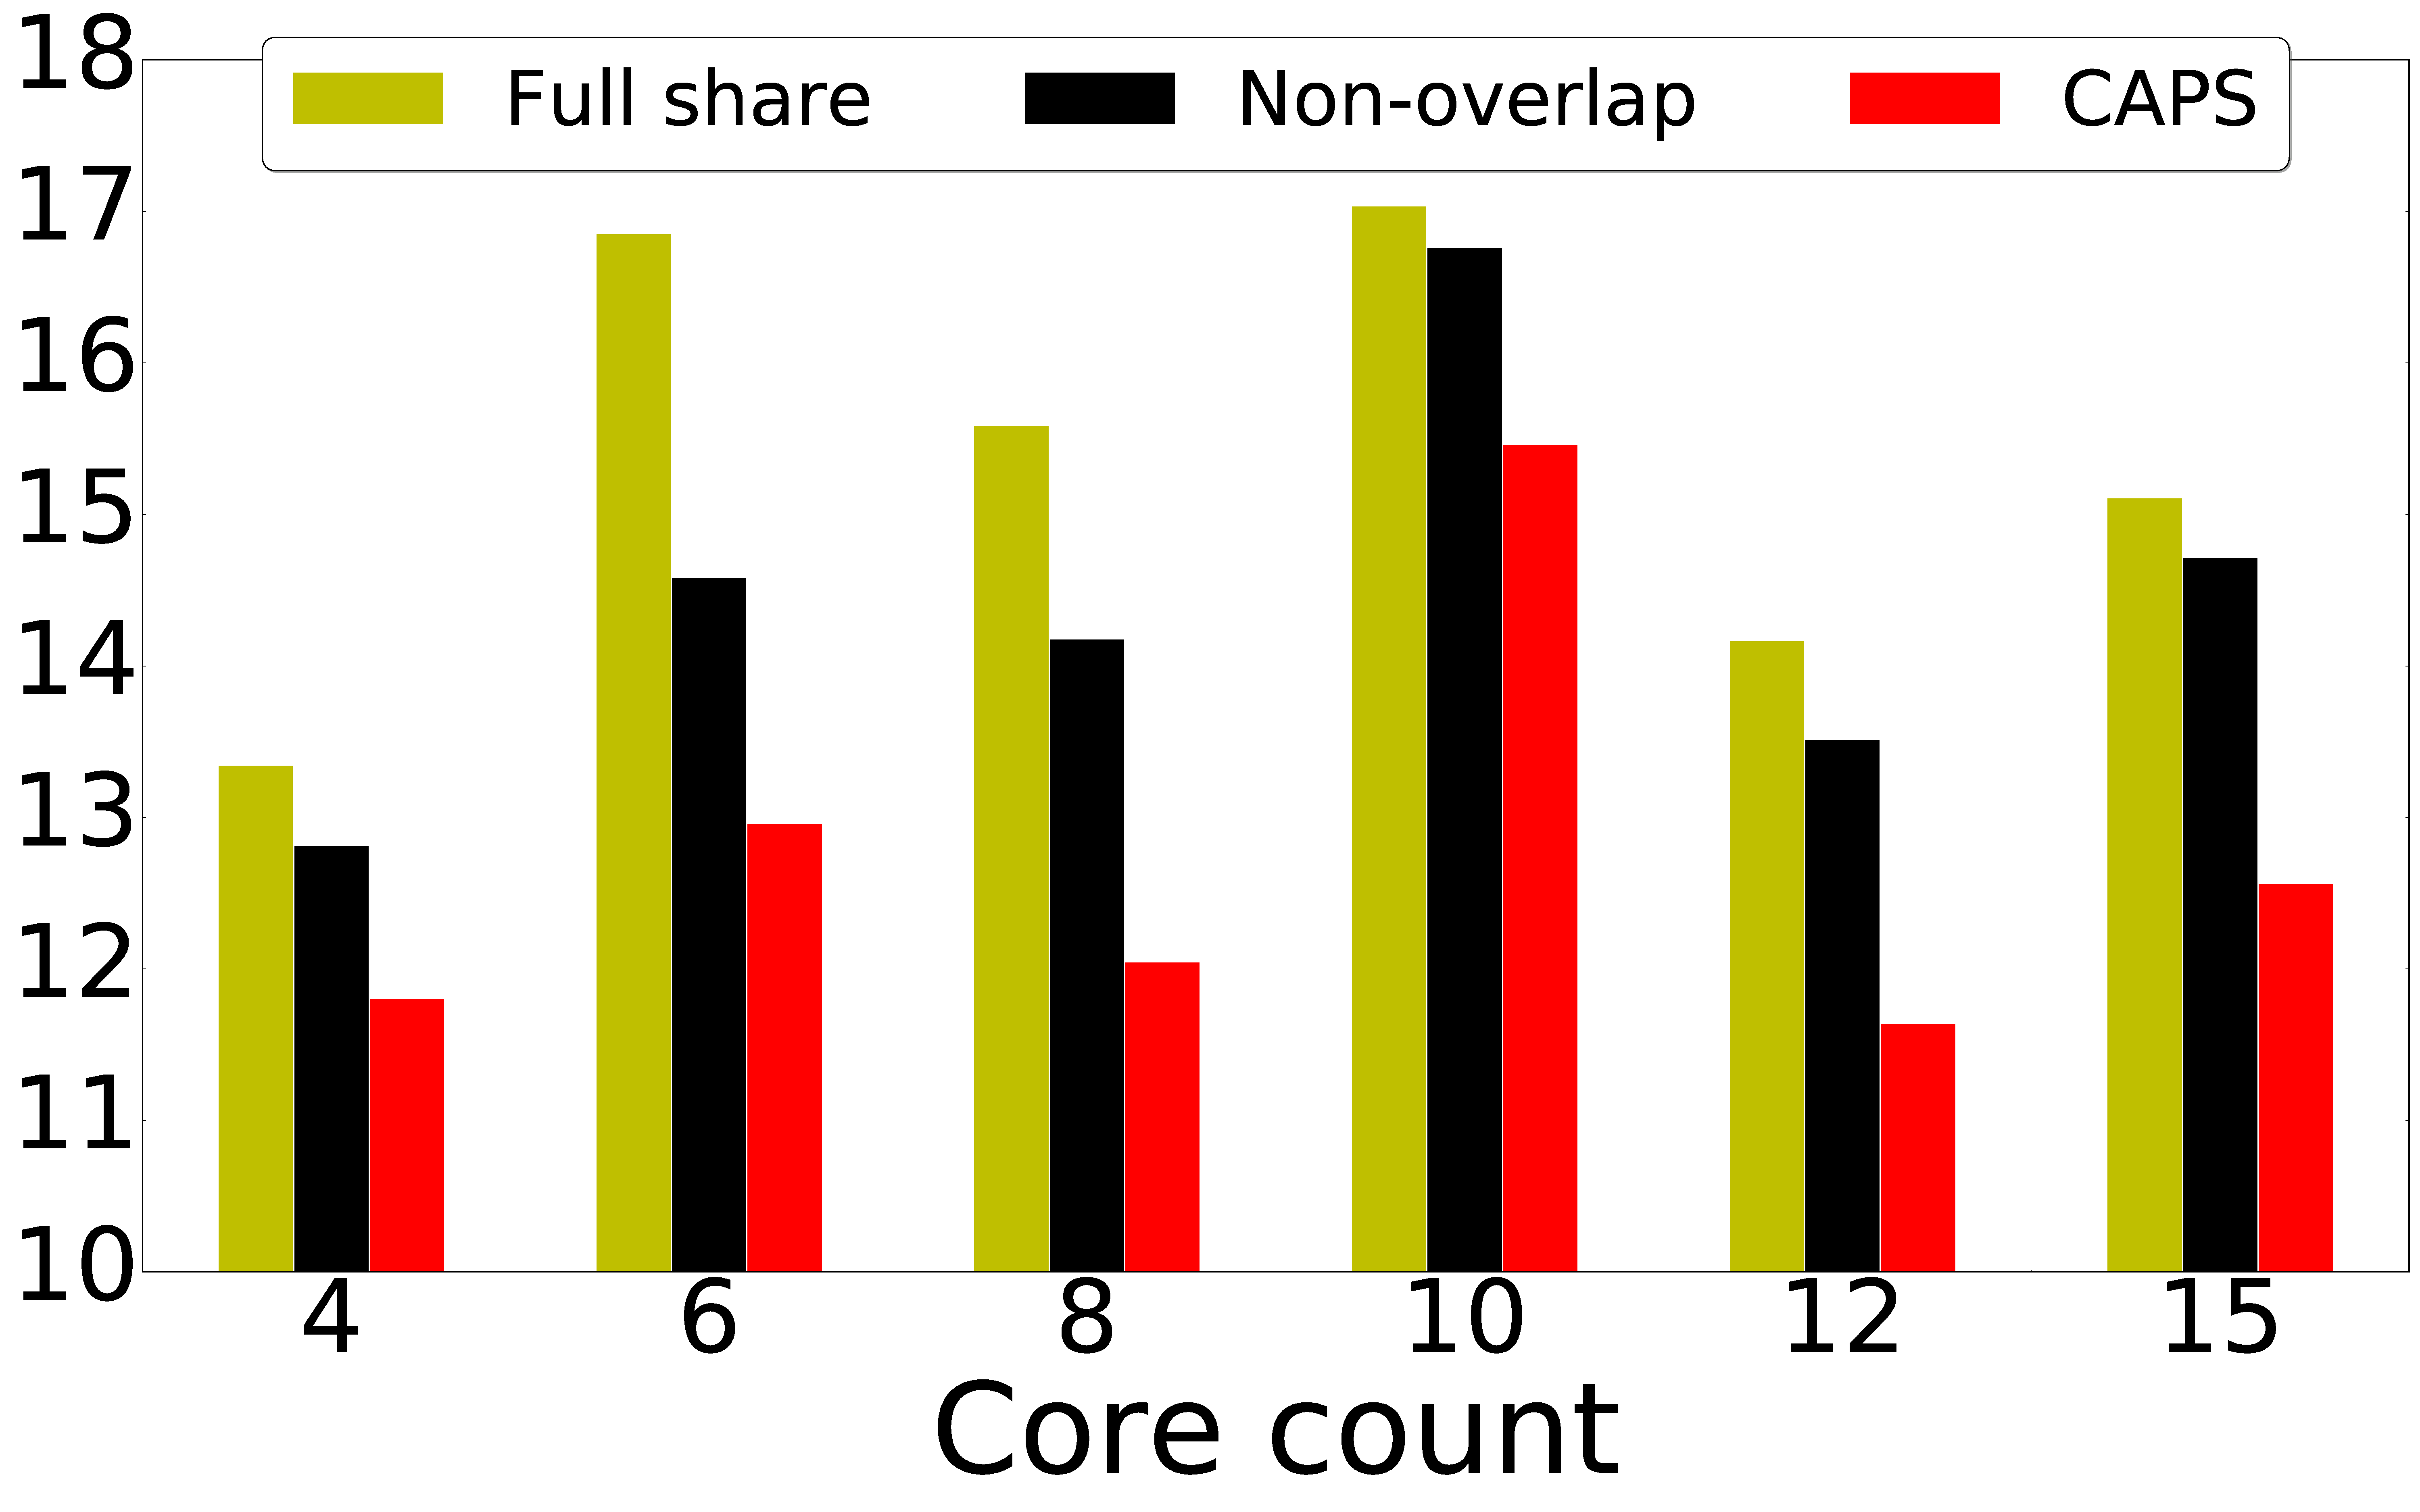
\includegraphics[width=0.9\linewidth]{figures/mpki.pdf}
        \caption{Average MPKI}
    \end{subfigure}%
    \begin{subfigure}[b]{0.5\linewidth}
        \centering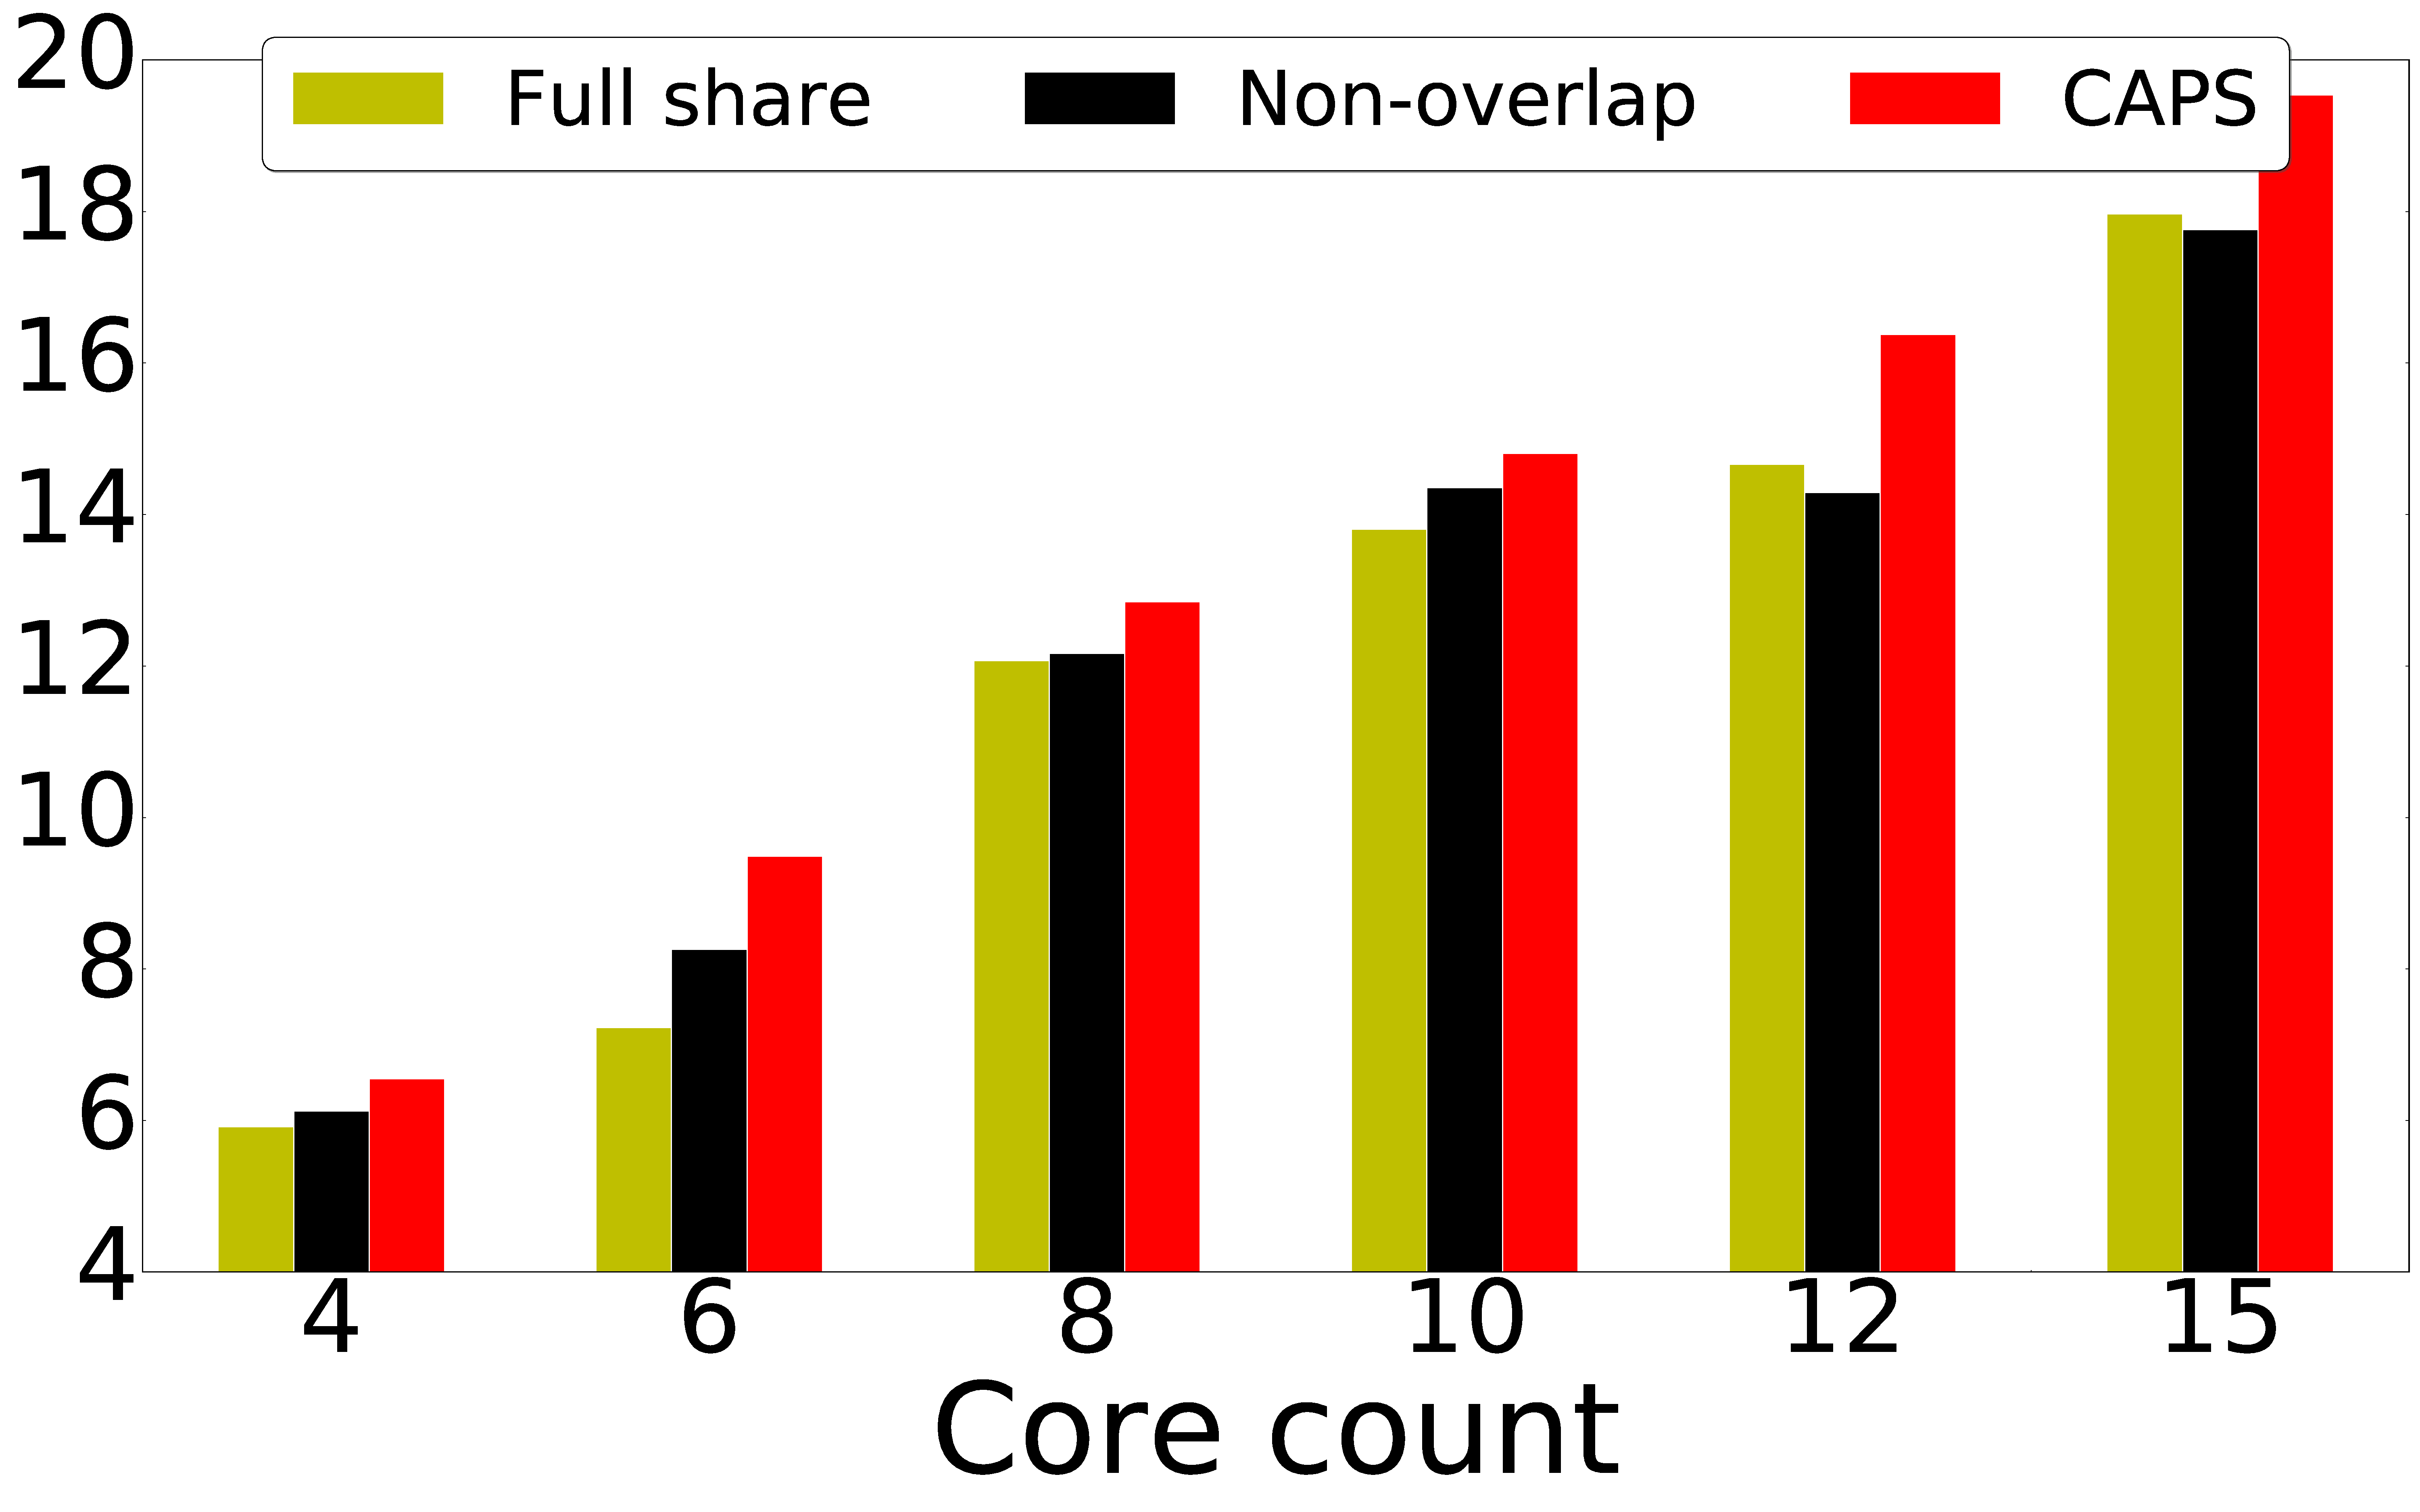
\includegraphics[width=0.9\linewidth]{figures/ipc.pdf}
        \caption{Throughput}
    \end{subfigure}
    \begin{subfigure}[b]{0.5\linewidth}
        \centering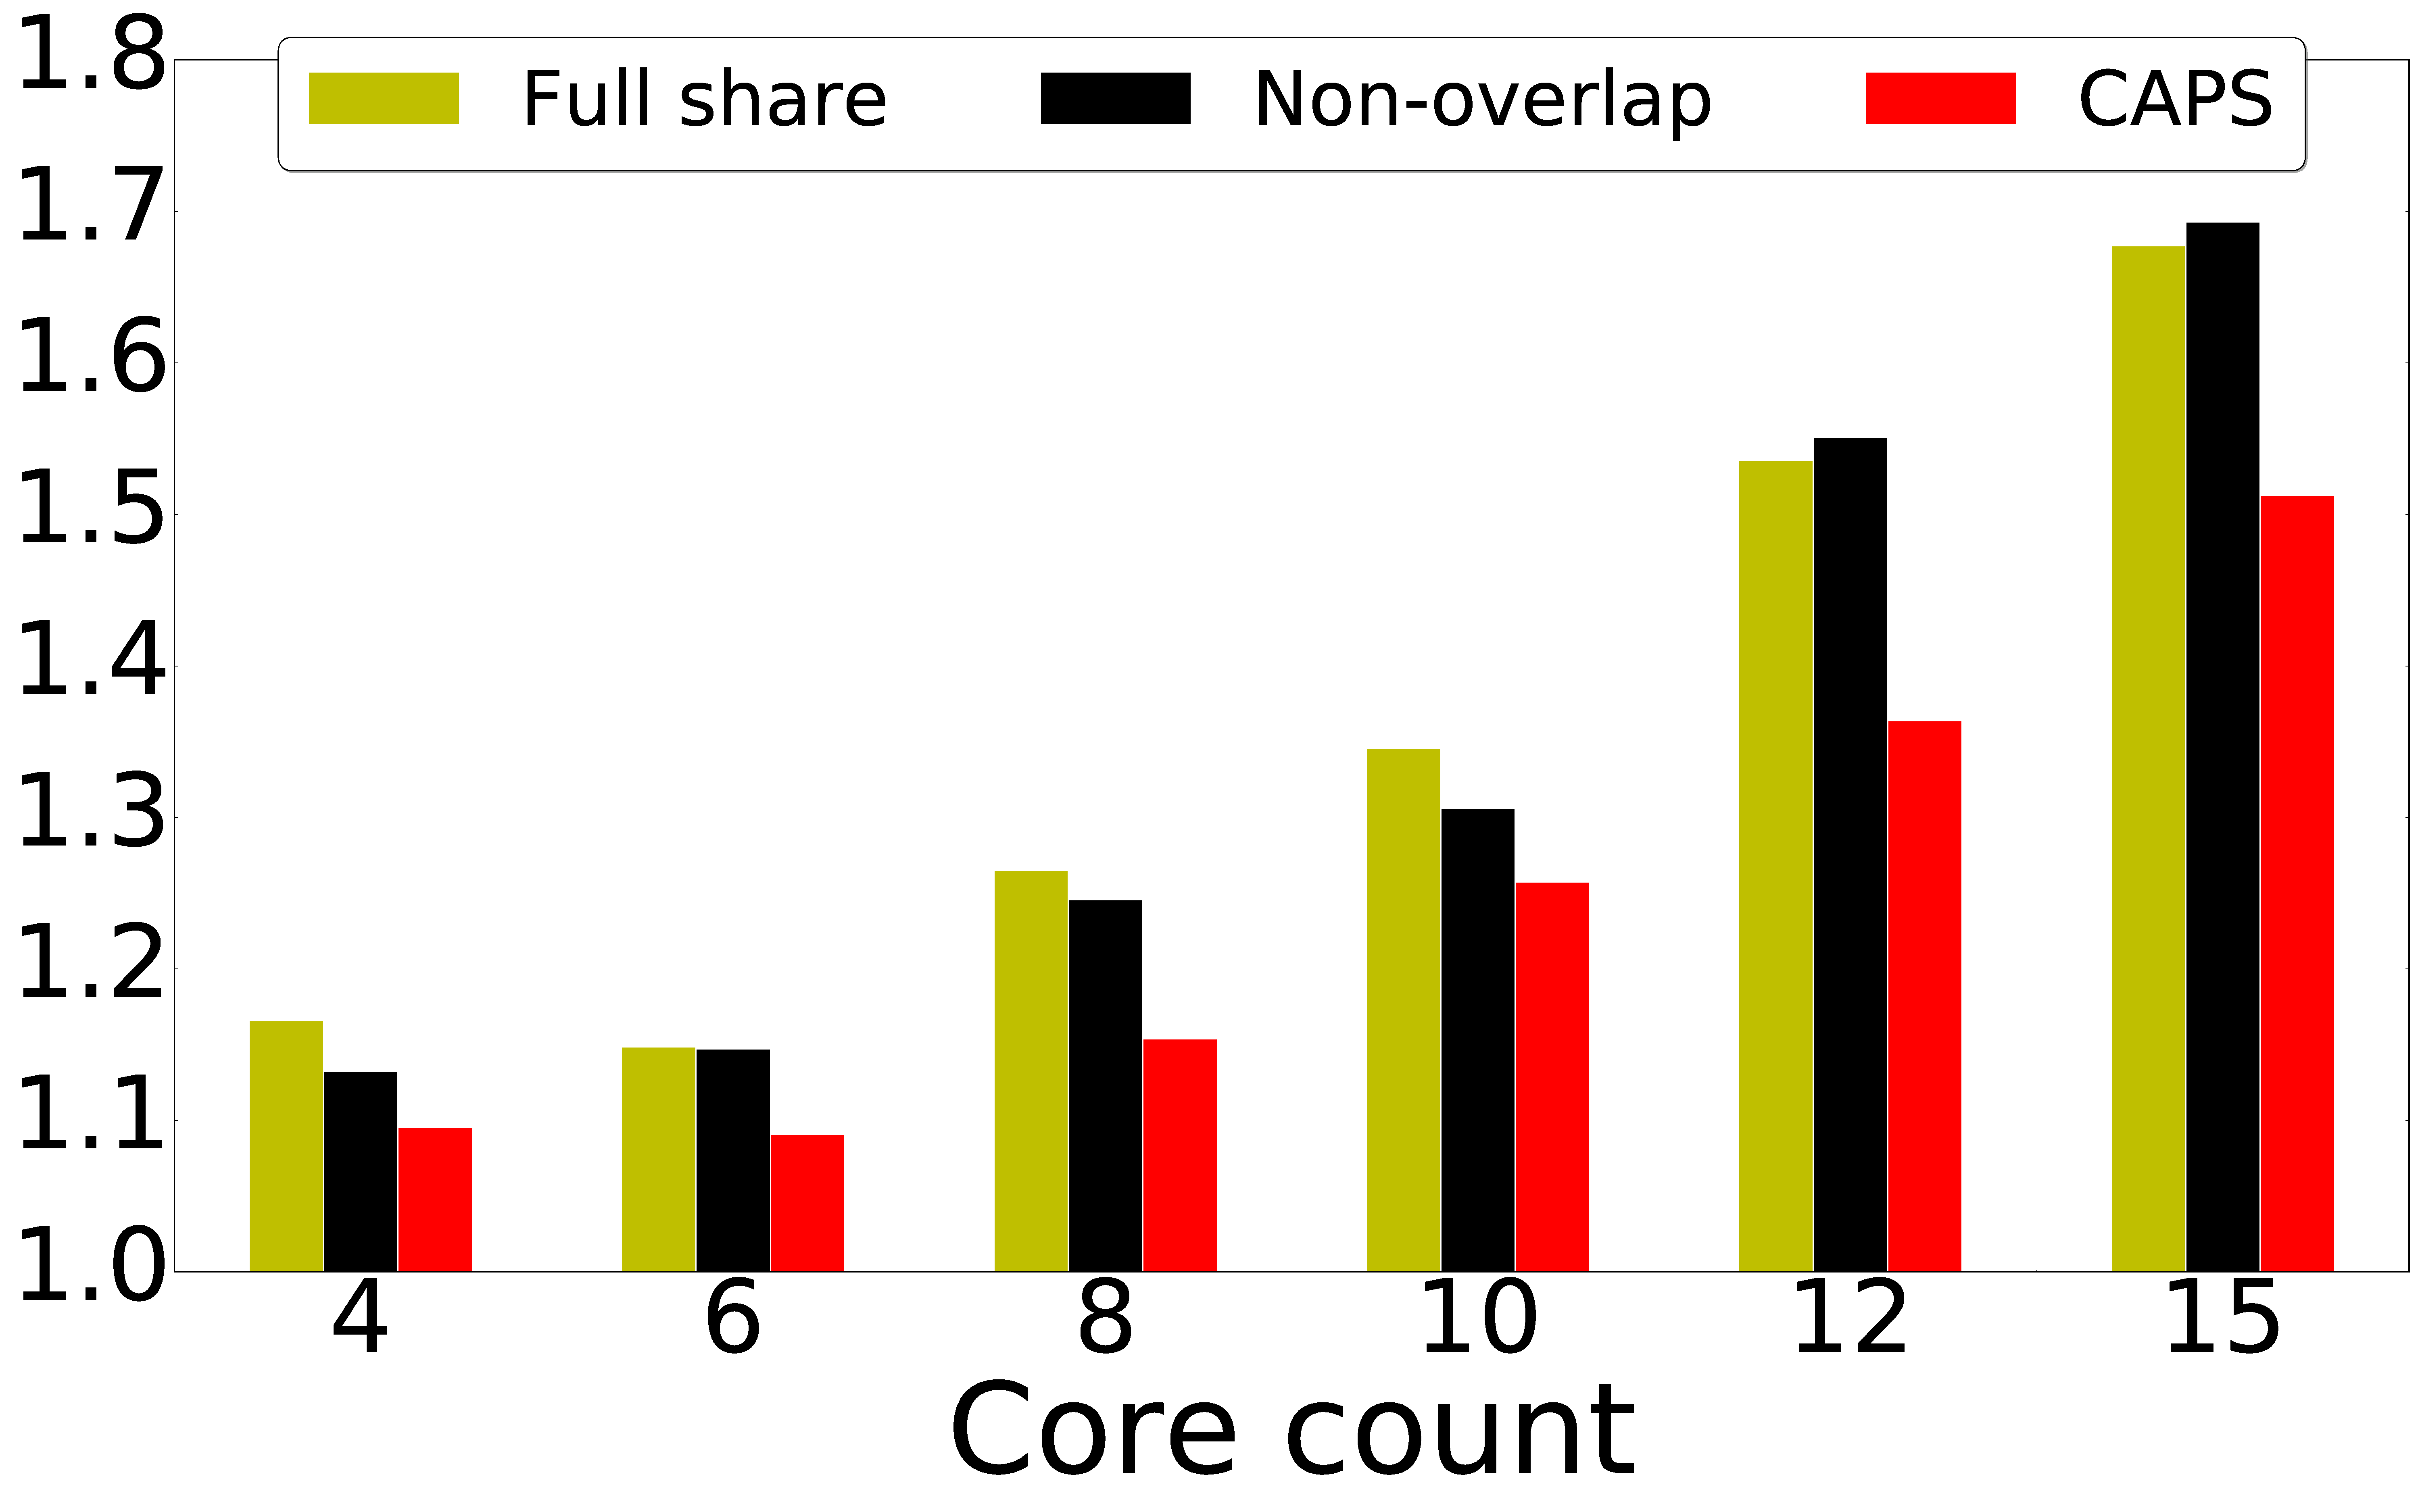
\includegraphics[width=0.9\linewidth]{figures/ws.pdf}
        \caption{Average slowdown}
    \end{subfigure}%
    \begin{subfigure}[b]{0.5\linewidth}
        \centering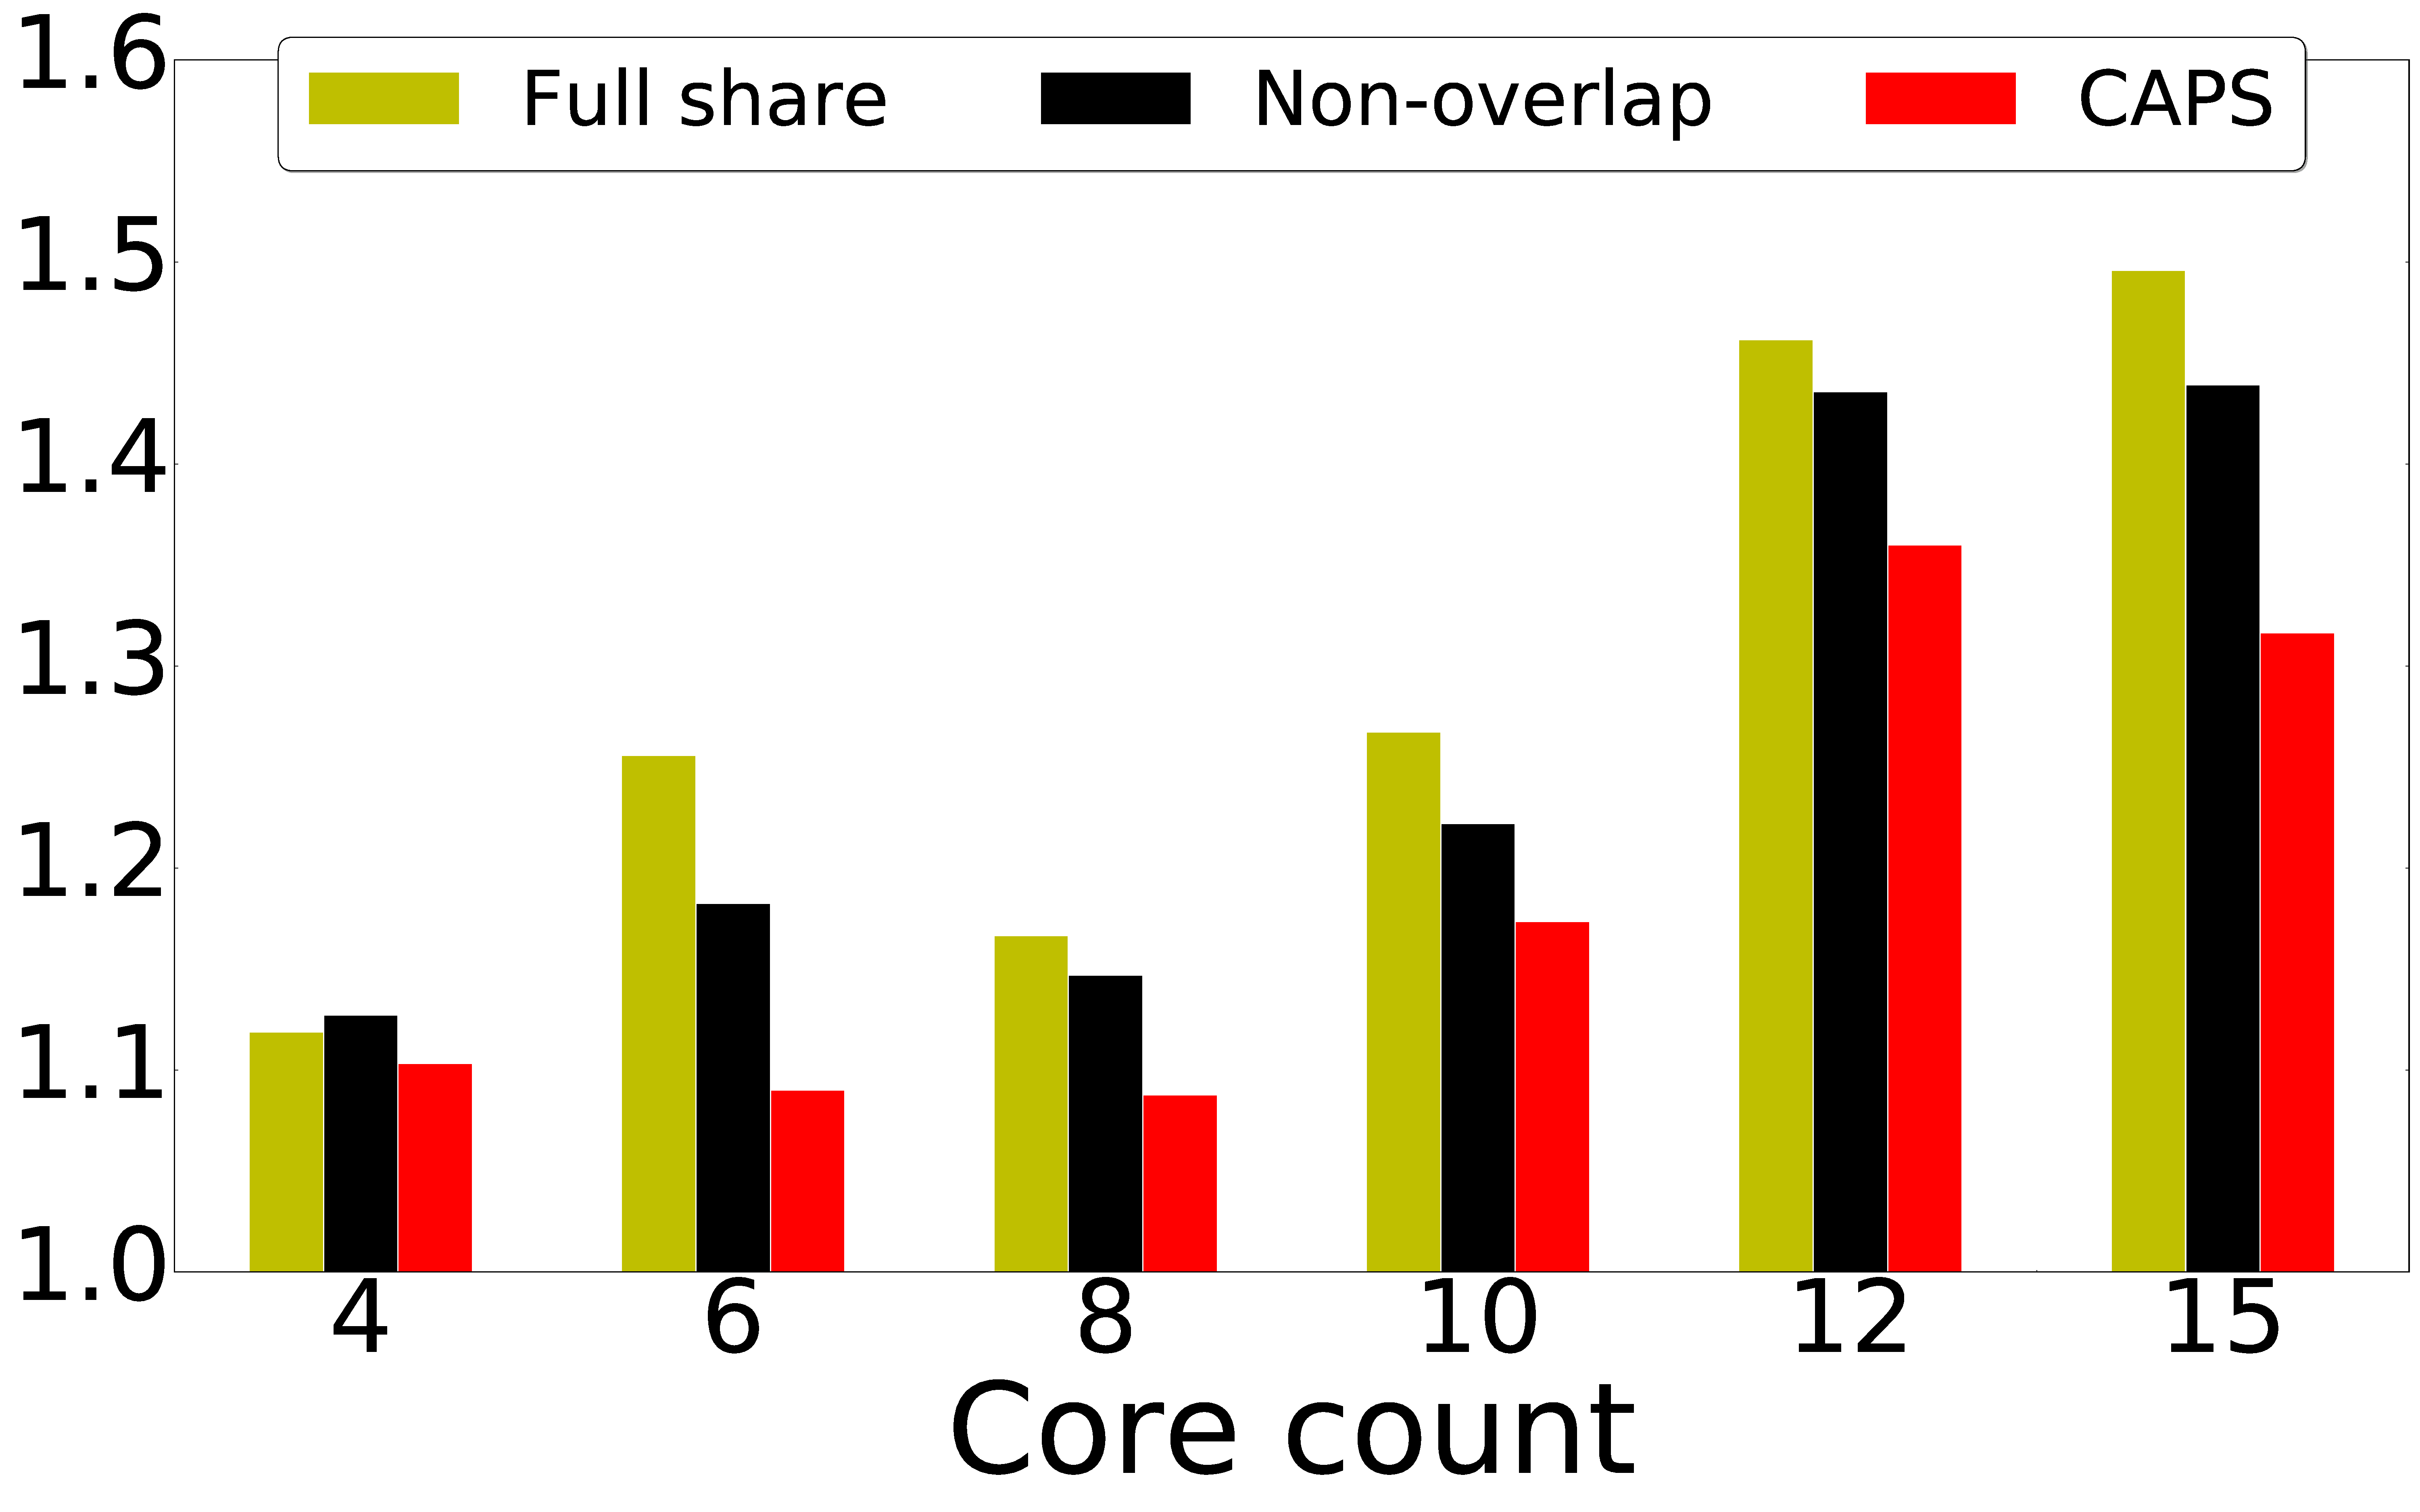
\includegraphics[width=0.9\linewidth]{figures/fs.pdf}
        \caption{Fair slowdown}
    \end{subfigure}
    \begin{subfigure}[b]{0.5\linewidth}
        \centering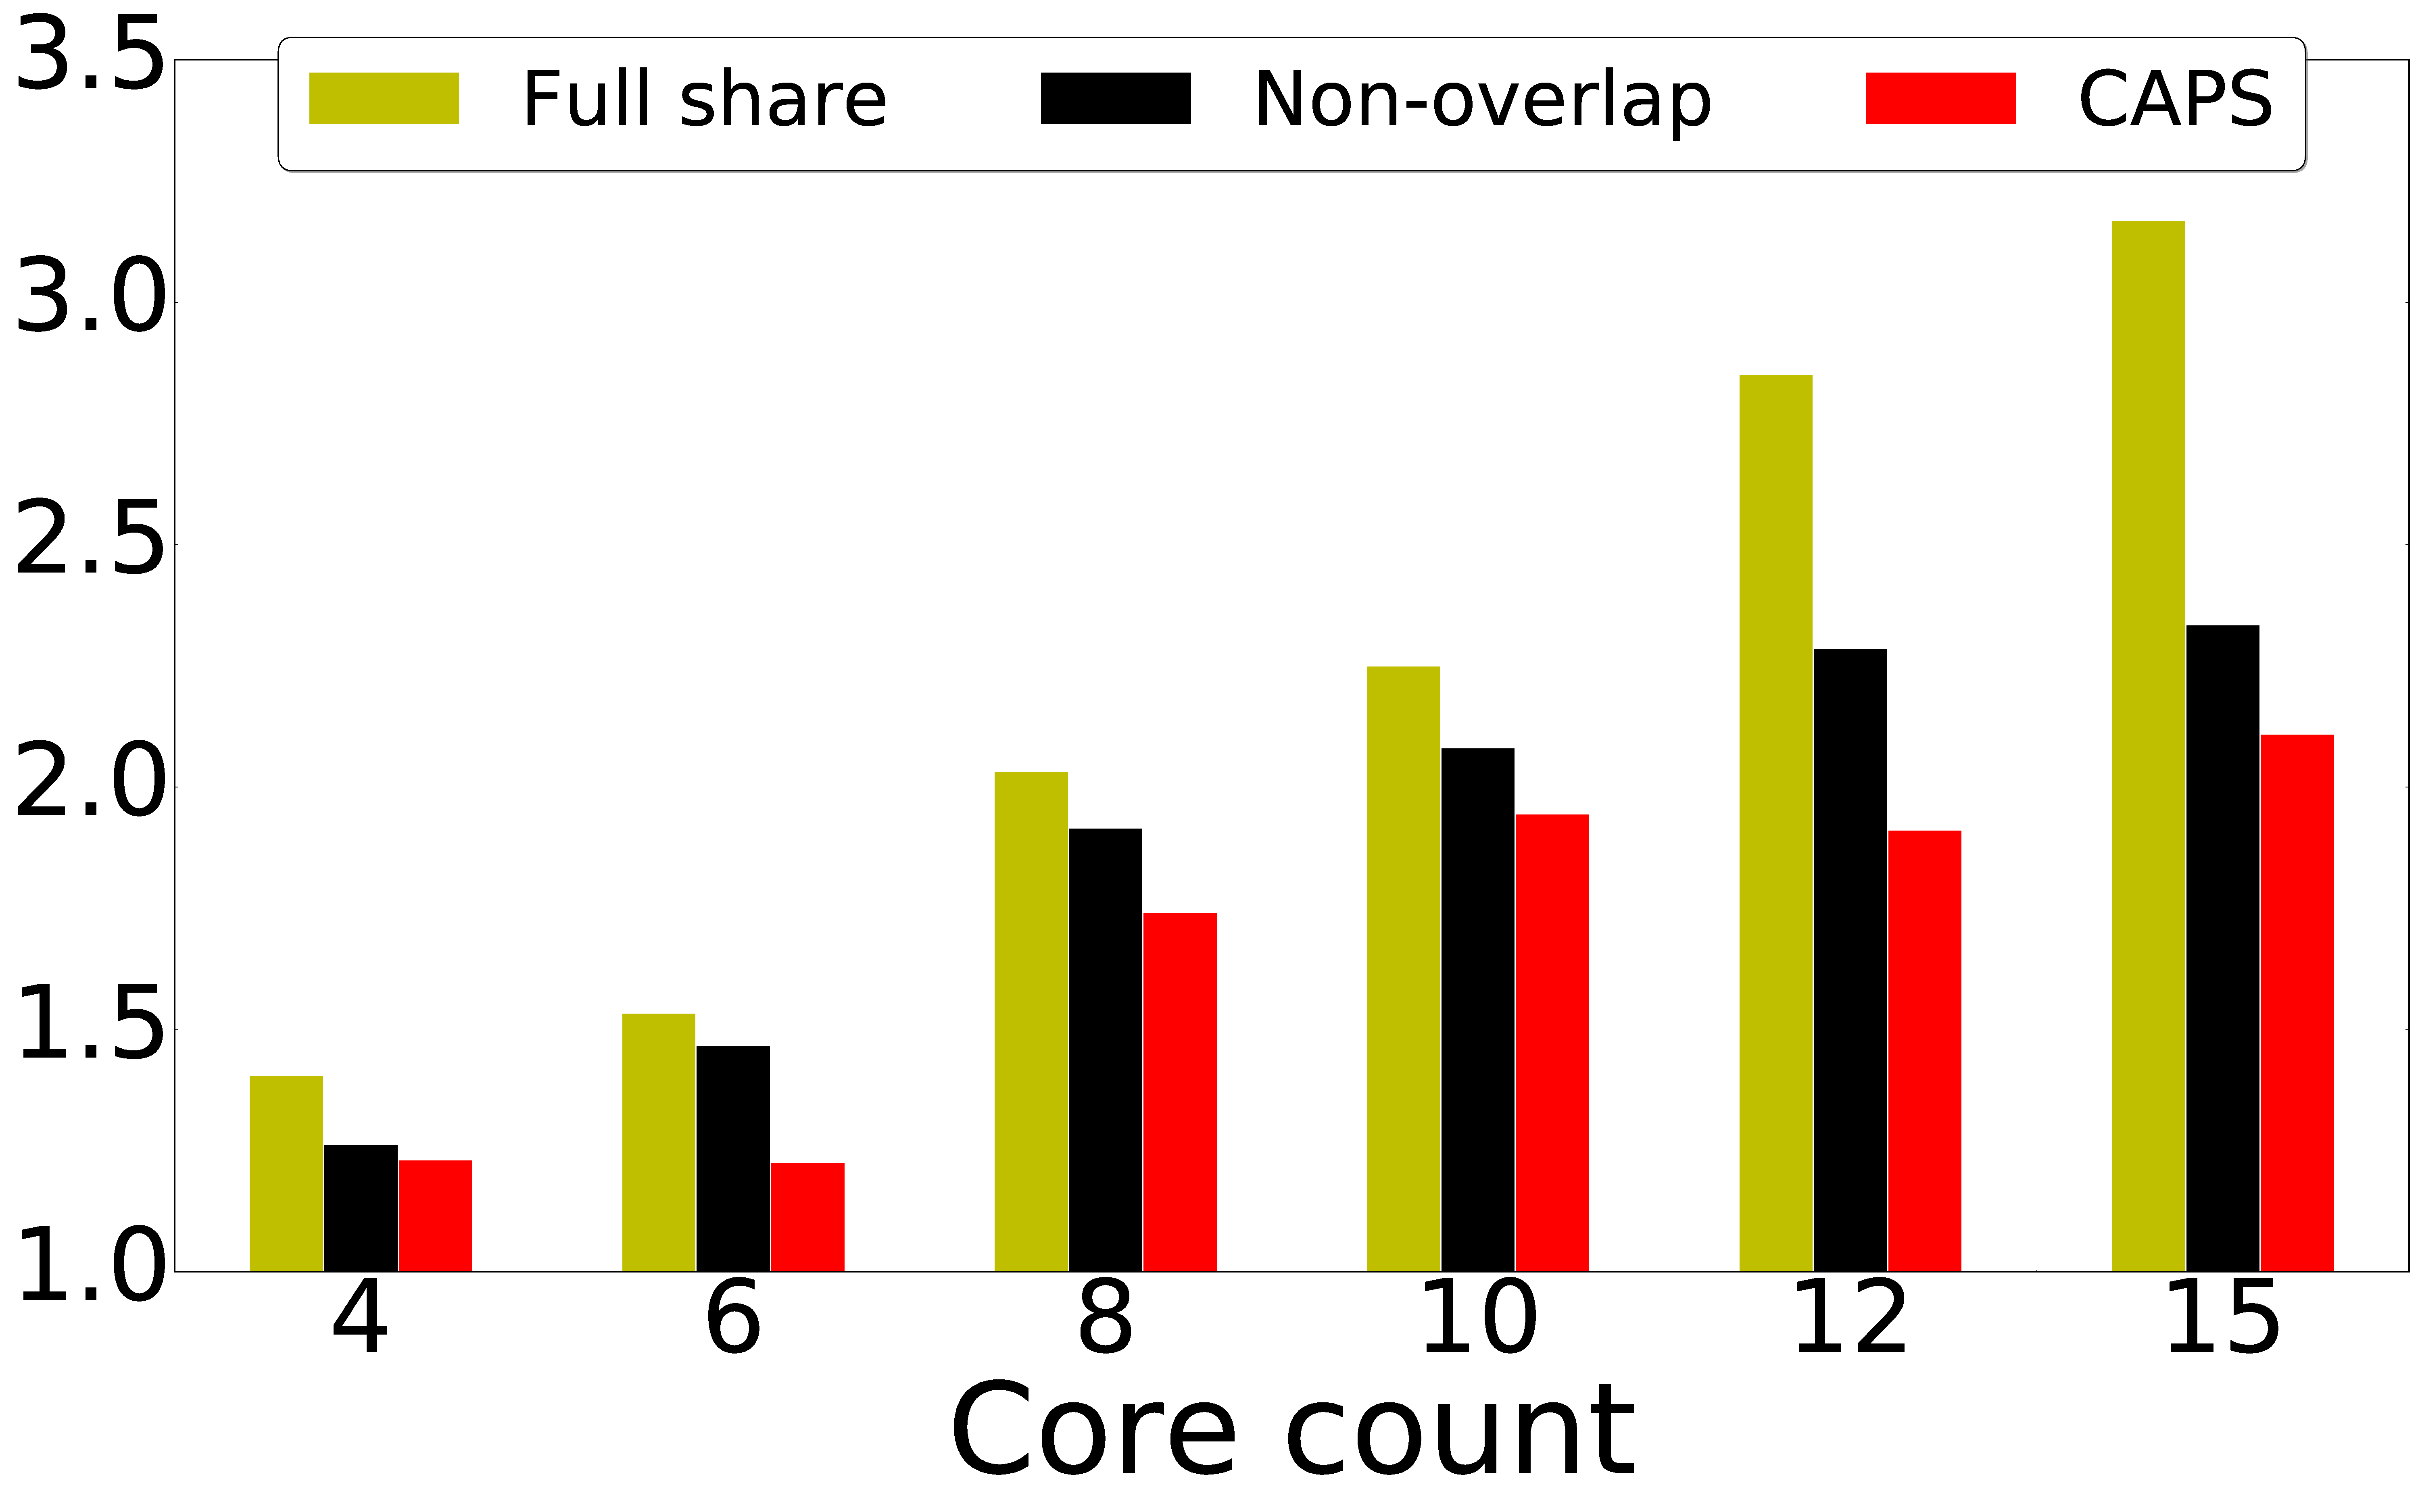
\includegraphics[width=0.9\linewidth]{figures/ms.pdf}
        \caption{Maximum slowdown}
    \end{subfigure}
    \caption{完全重叠、不重叠与CAPS部分重叠方案在不同核数下的5个优化指标对比}
    \label{fig:core_count}
\end{figure}

从图中可以看出,无论核数多少,CAPS生成的部分重叠方案基本上都是效果最好的方案。其次,随着核数的增加,对LLC的竞争愈发增加,性能下降也更为明显,这也给了CAPS更大的优化空间。可以看出随着核数的增加,CAPS对比自由竞争和不重叠的优势更加显著。特别地,在Average slowdown上,4核下CAPS平均可以把自由竞争下的1.166的Slowdown降低到1.095,优化效果达6.1\%,而在12核下,CAPS可以把1.536的Slowdown降低到1.364,提升效果达11.2\%。

不重叠分配方案在大多数情况下比自由竞争要稍微好一些。但是,随着核数的增加,不重叠方案的优化效果会越来差,在某些情况下甚至会起到反作用,比如在Average slowdown指标下12核和15核的情况,不重叠方案都比自由竞争还要差一点。之所以不重叠方案在高核数下效果不好,是因为其粒度过粗,不具有很好的扩展性。极端情况下当核数等于缓存路数的时候,该方案只能给每个核分配一个路,就彻底失去了灵活性,而只能起到隔离效果。与之不同的是,对于Maximum slowdown这个指标来说,不重叠方案相比于自由竞争方案能持续提供优化效果,这是因为该指标偏向于QoS,更加注重隔离干扰。在并发负载中,最严重Slowdown往往是由一个缓存非常敏感的程序引起的。不重叠的分配方案可以限制高污染性程序的缓存使用,使得敏感程序免受它们的干扰,这样Maximum slowdown就获得了优化。诚然如此,不重叠方案在各方面也是全面落后于CAPS部分重叠方案的。

可以观察到一个有趣的现象,在Fair slowdown下,8核相比6核的Slowdown反而更小了。这里的原因在于该指标注重公平性,因为不同的测试程序组合可能会对公平性造成不同的影响,新增的程序使得公平性更好或者更坏都有可能。  

\section{工作负载差异性的评估分析}

在本节中,我们对不同的工作负载组合进行评估分析。本评估重点针对10核的工作负载,通过不同的A类程序、B类程序和C类程序配比,每个负载包含10个各异的测试程序,一共产生25种组合。我们将这25个工作负载分别标记为“D1”到“D25”,配比详情如表\ref{tab:10w}所示。


\begin{table}[htbp]
\caption{10核工作负载配比表}
\label{tab:10w}
\centering
\begin{tabularx} {0.8\linewidth}{|X|l|l|l| } 
 \hline
 Label & TypeA & TypeB & TypeC \\
 \hline
D1 & 0 & 5 & 5 \\
\hline 
D2 & 2 & 2 & 6 \\
\hline 
D3, D4 & 2 & 5 & 3 \\
\hline 
D5, D6, D7 & 3 & 3 & 4 \\
\hline 
D8 & 3 & 4 & 3 \\
\hline 
D9, D10, D11 & 3 & 5 & 2 \\
\hline 
D12, D13, D14 & 4 & 3 & 3 \\
\hline 
D15, D16 & 5 & 0 & 5 \\
\hline 
D17 & 5 & 2 & 3 \\
\hline 
D18 & 5 & 3 & 2 \\
\hline 
D19 & 5 & 5 & 0 \\
\hline 
D20, D21, D22 & 6 & 2 & 2 \\
\hline 
D23 & 7 & 2 & 1 \\
\hline 
D24 & 8 & 1 & 1 \\
\hline 
D25 & 9 & 1 & 0 \\
\hline 
\end{tabularx}
\end{table}

\begin{figure}[htbp] 
    \centering
    \begin{subfigure}[b]{1\linewidth}
        \centering\includegraphics[width=0.95\linewidth]{figures/d20_miss.pdf}
        \caption{Average MPKI}
    \end{subfigure}
    \begin{subfigure}[b]{1\linewidth}
        \centering
\includegraphics[width=0.95\linewidth]{figures/d20_ipc.pdf}
        \caption{Throughput}
    \end{subfigure}
    \begin{subfigure}[b]{1\linewidth}
        \centering
\includegraphics[width=0.95\linewidth]{figures/d20_ws.pdf}
        \caption{Average slowdown}
    \end{subfigure}
    \begin{subfigure}[b]{1\linewidth}
        \centering
\includegraphics[width=0.95\linewidth]{figures/d20_fs.pdf}
        \caption{Fair slowdown}
    \end{subfigure}
    \begin{subfigure}[b]{1\linewidth}
        \centering\includegraphics[width=0.95\linewidth]{figures/d20_ms.pdf}
        \caption{Maximum slowdown}
    \end{subfigure}
    \caption{完全重叠、不重叠与CAPS部分重叠方案在10个并发负载下的5个优化指标对比}
    \label{fig:10w}
\end{figure}

实验结果如图\ref{fig:10w}所示。可以看到,CAPS基本上在每种工作负载的每种指标上都处于领先地位,除了D11的吞吐量。A类程序属于缓存敏感型,而B类属于不敏感且污染型, 当A类程序和B类程序在竞争使用LLC时,A类程序往往会因为B类程序的影响而导致严重的性能下降。所以当一个工作负载中A类和B类程序比较多时,自由竞争情况下的性能下降往往会比较严重,但在这种情况下CAPS往往能起到很好的优化效果。而在C类程序较多时,由于本身自由竞争下的性能损失也不大,所以留给CAPS的优化空间也较小。

同时,我们还观察到只要有一个污染性很大的程序就会对整个工作负载造成较大的影响。例如,D21和D18两个负载只差一个462.libquantum测试程序,D18把D21中的473.astar替换成462.libquantum,其余的程序都一样。然而,自由共享下的各项指标都变差了很多。462.libquantum是一个典型的B类程序,它的局部性较差,并不会从缓存占用中收益很多,但同时它的访存频率很高,在竞争情况下会占据大量空间,从而污染整个缓存空间。幸运的是,CAPS可以自动识别到这样的程序,然后限制它们的缓存使用,可以看到对于D18这组工作负载,CAPS都大大优化了5项指标的数值。

\section{个案分析}

在本节中,我们拿一个10核工作负载做更详细的分析。我们选择研究的负载是上节提到的D10,它是由10个程序组成:401.bzip2, 403.gcc, 429.mcf, 436.cactus, 465.tonto, 410.bwaves, 434.zeusmp, 437.leslie3d, 459.GemsFDTD和462.libquantum。这些程序中,前5个是A类敏感型程序,后5个是B类污染型程序。因为C类程序既不敏感也不污染,对整体的工作负载影响不大,考虑到典型性,所以本个案中就没有包含C类程序。图\ref{fig:case_scheme}展示了CAPS针对Throughput和Fair slowdown这两个优化指标所生成的方案。可以看到各个分配会有部分的重叠。光从分配方案上很难看出每个程序的实际占用是多少。因为一个看似很大的分配可能由于与多个程序竞争,实际占用的缓存空间会很小。为了更好的展示这两种分配方案的实际效果,我们使用缓存监控技术(CMT)实时测得了各个程序的实际缓存占用,这两种方案下以及自由竞争时各个程序的实际平均缓存占用如图\ref{fig:case_occu}所示。

\begin{figure}[htbp]
\centering
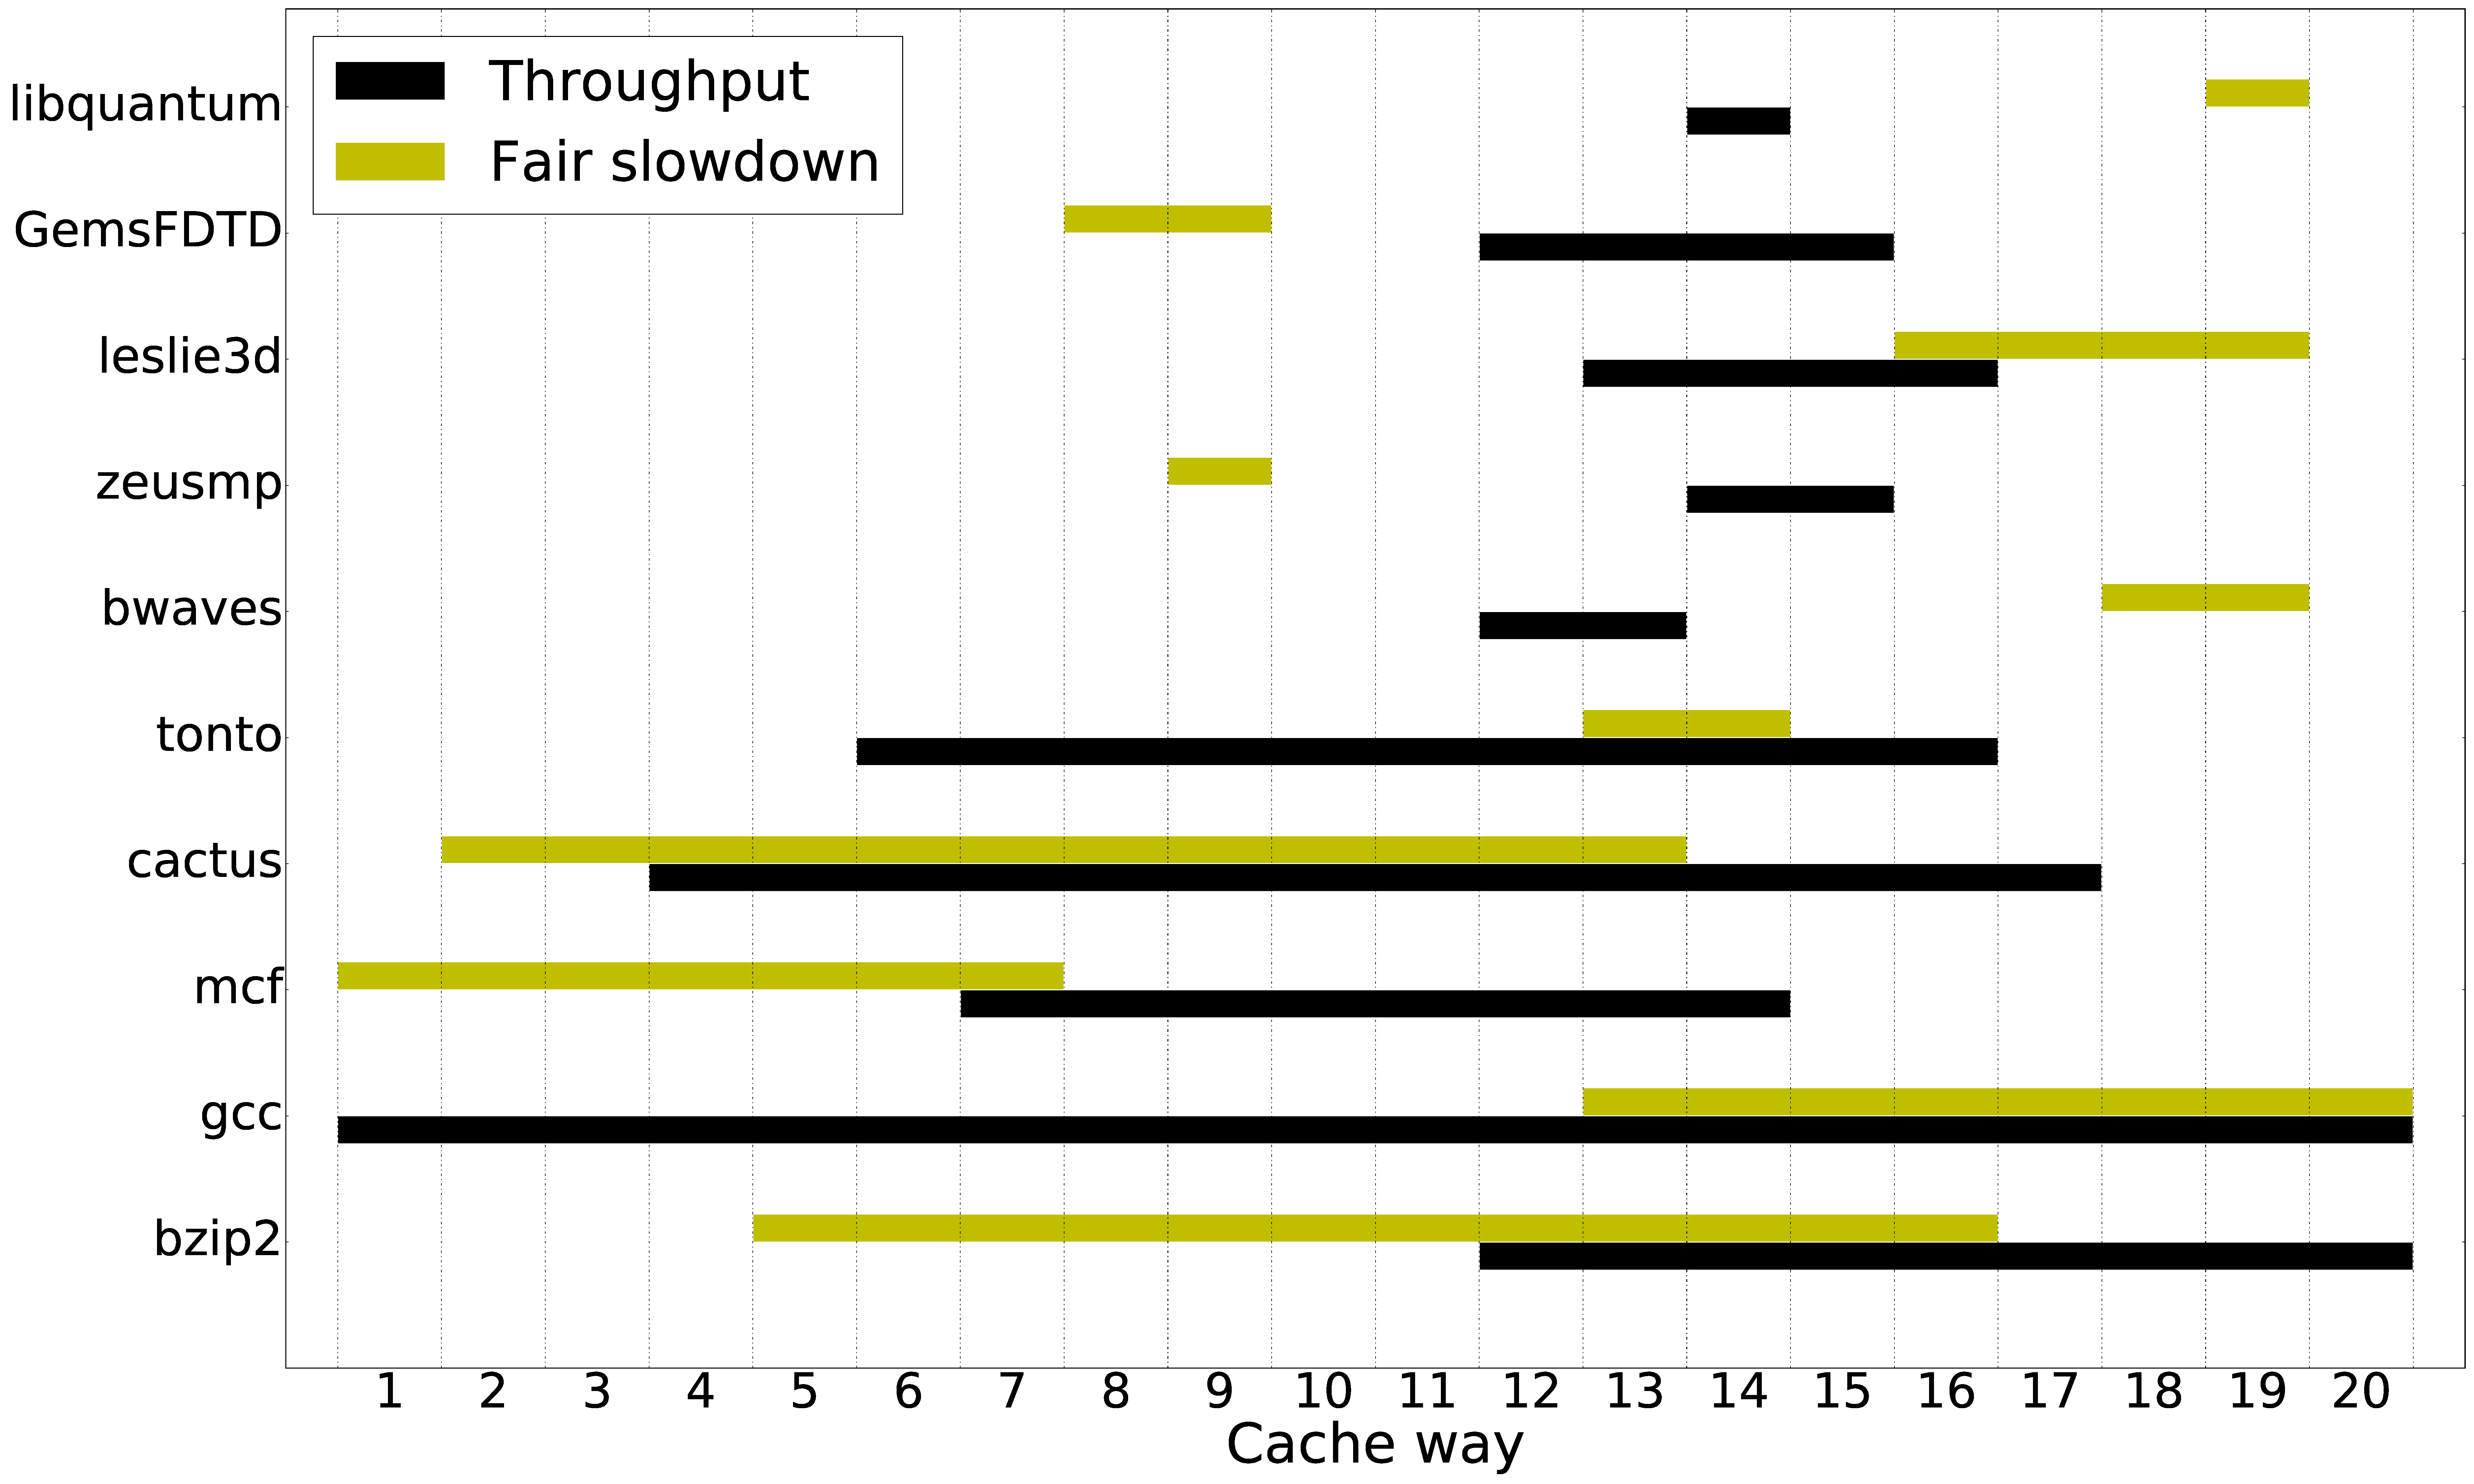
\includegraphics[width=0.95\columnwidth]{figures/case_study.pdf}
\caption{两种分别针对Throughput和Fair slowdown的CAPS分配方案}
\label{fig:case_scheme}
\end{figure} 

\begin{figure}[htbp]
\centering
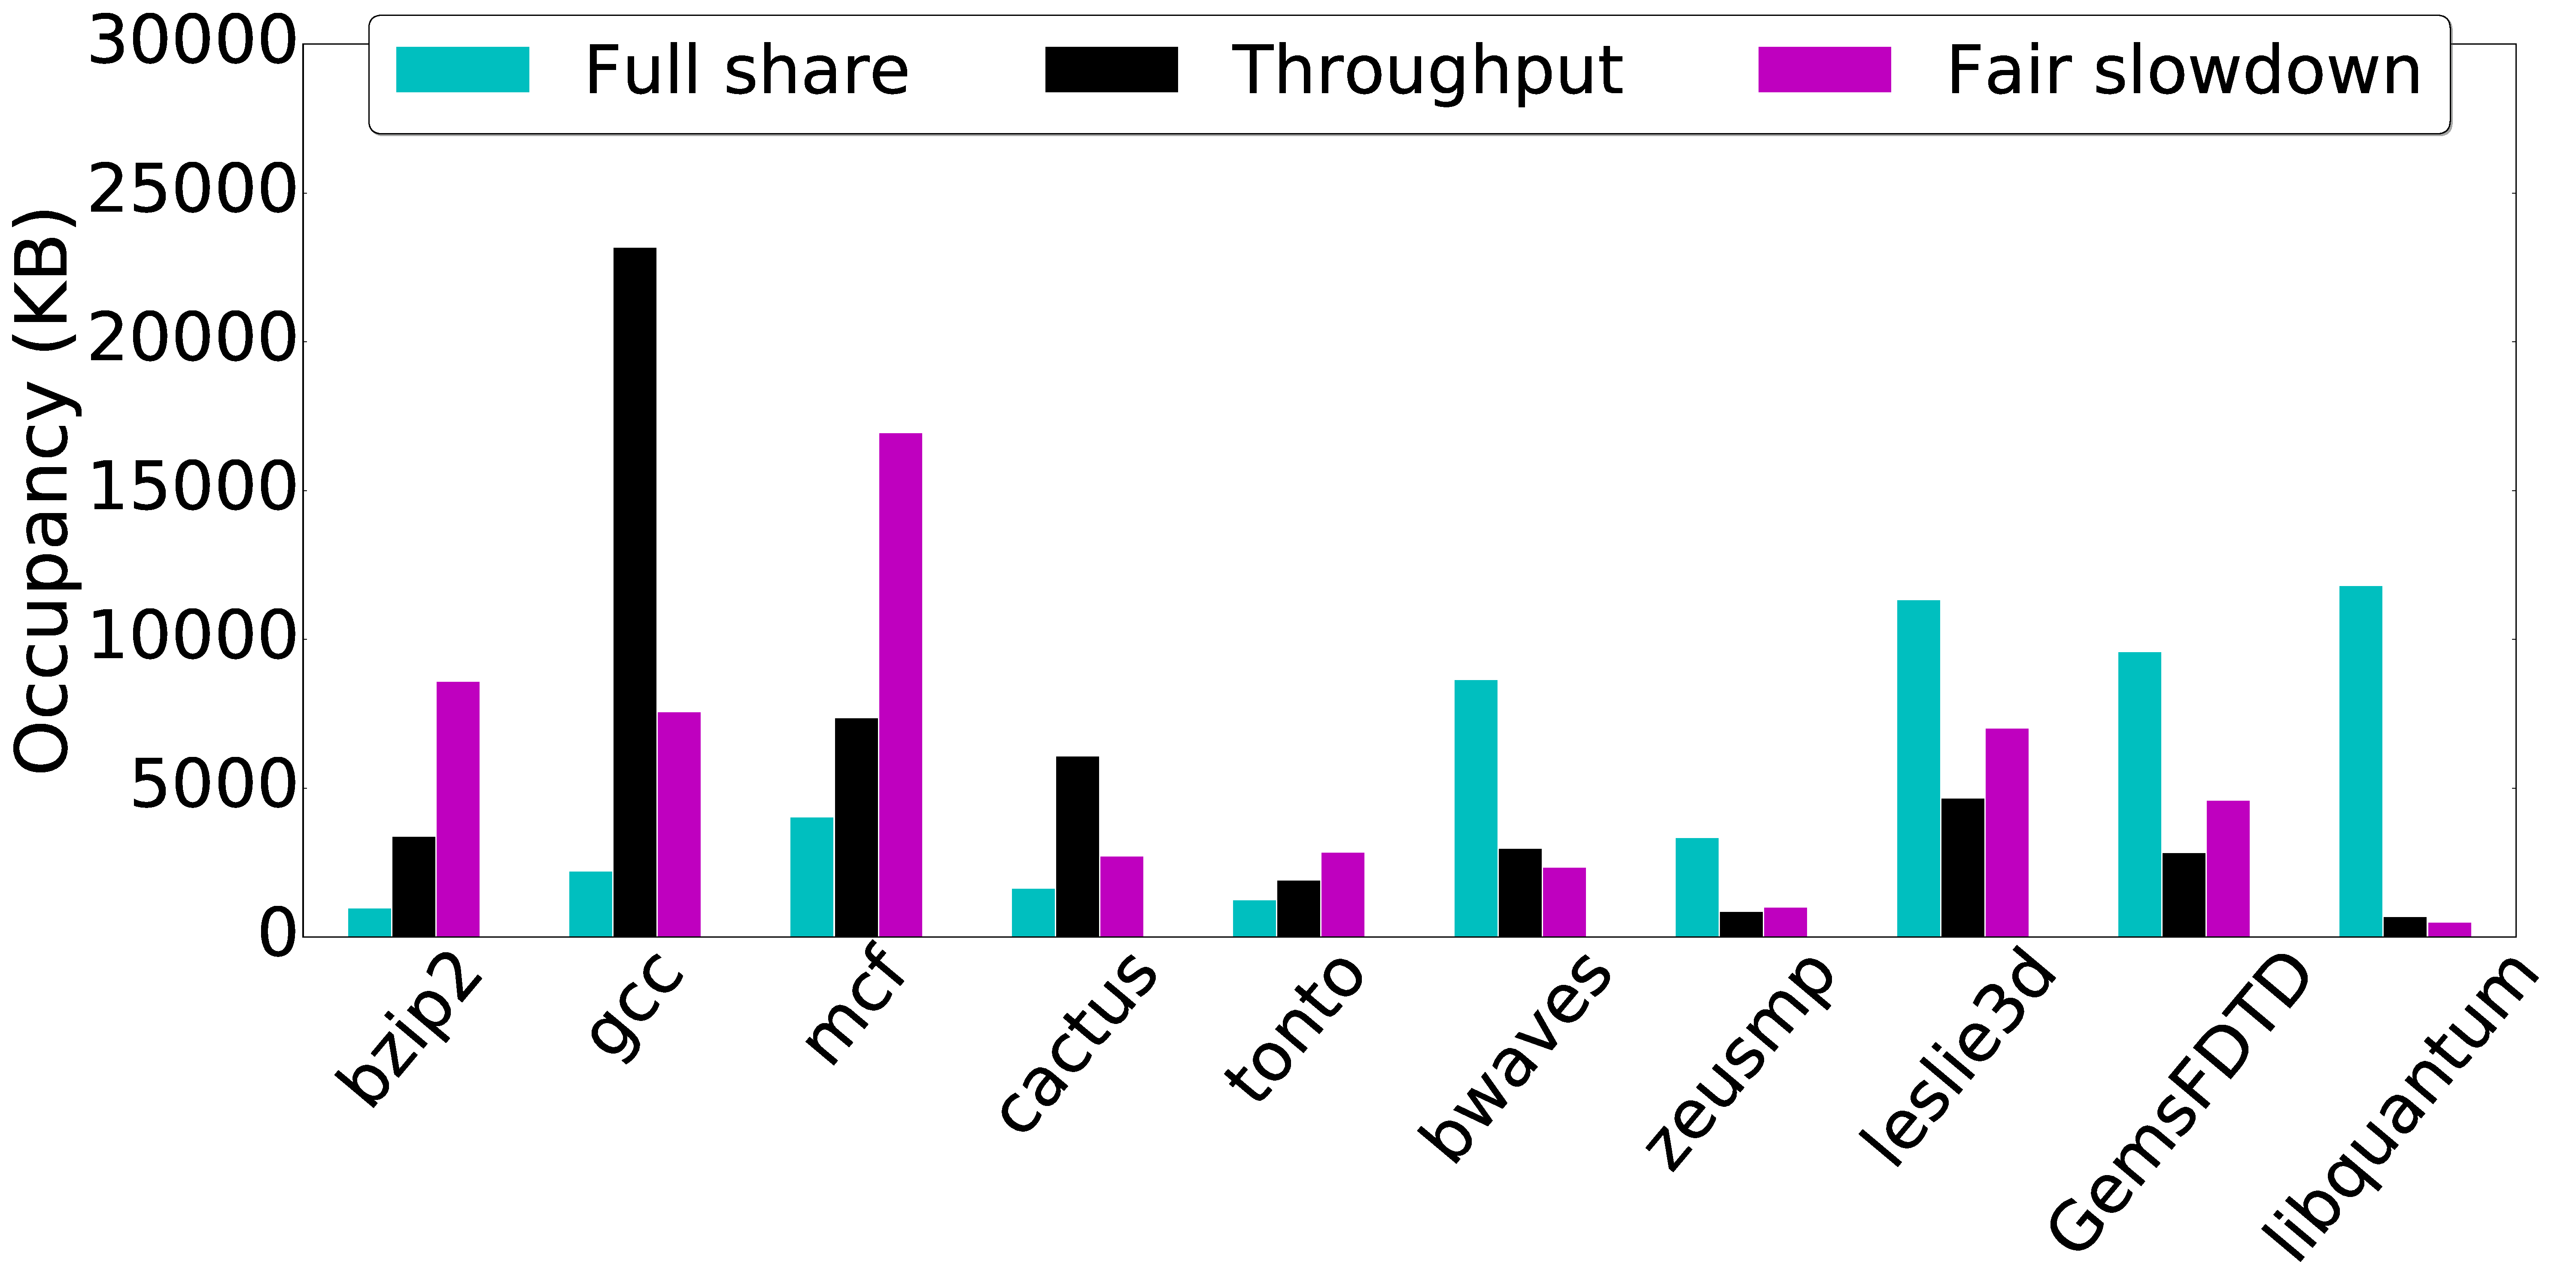
\includegraphics[width=0.9\linewidth]{figures/occ.pdf}
\caption{在自由竞争以及CAPS生成的Throughput和Fair slowdown方案下每个程序的实际缓存占用}
\label{fig:case_occu}
\end{figure} 

可以看出,无论是针对Throughput还是针对Fair slowdown的方案都为A类程序分配了较大的缓存空间,同时限制B类程序的缓存使用,这符合一般缓存优化的逻辑。正如所预料的,测试结果表明5个A类程序的IPC相比于完全竞争的情况都得到了显著的提高,同时B类程序虽然缓存空间被限制在较小的区域,但总体IPC变化幅度不大,所以工作负载总体性能指标就会获得提高,在图\ref{fig:case_ipc}中可以明显观察到这种趋势。然而,无论是针对何种目标的优化,CAPS都会自动地发现并限制B类污染性程序的缓存使用。


\begin{figure}[htbp]
\centering
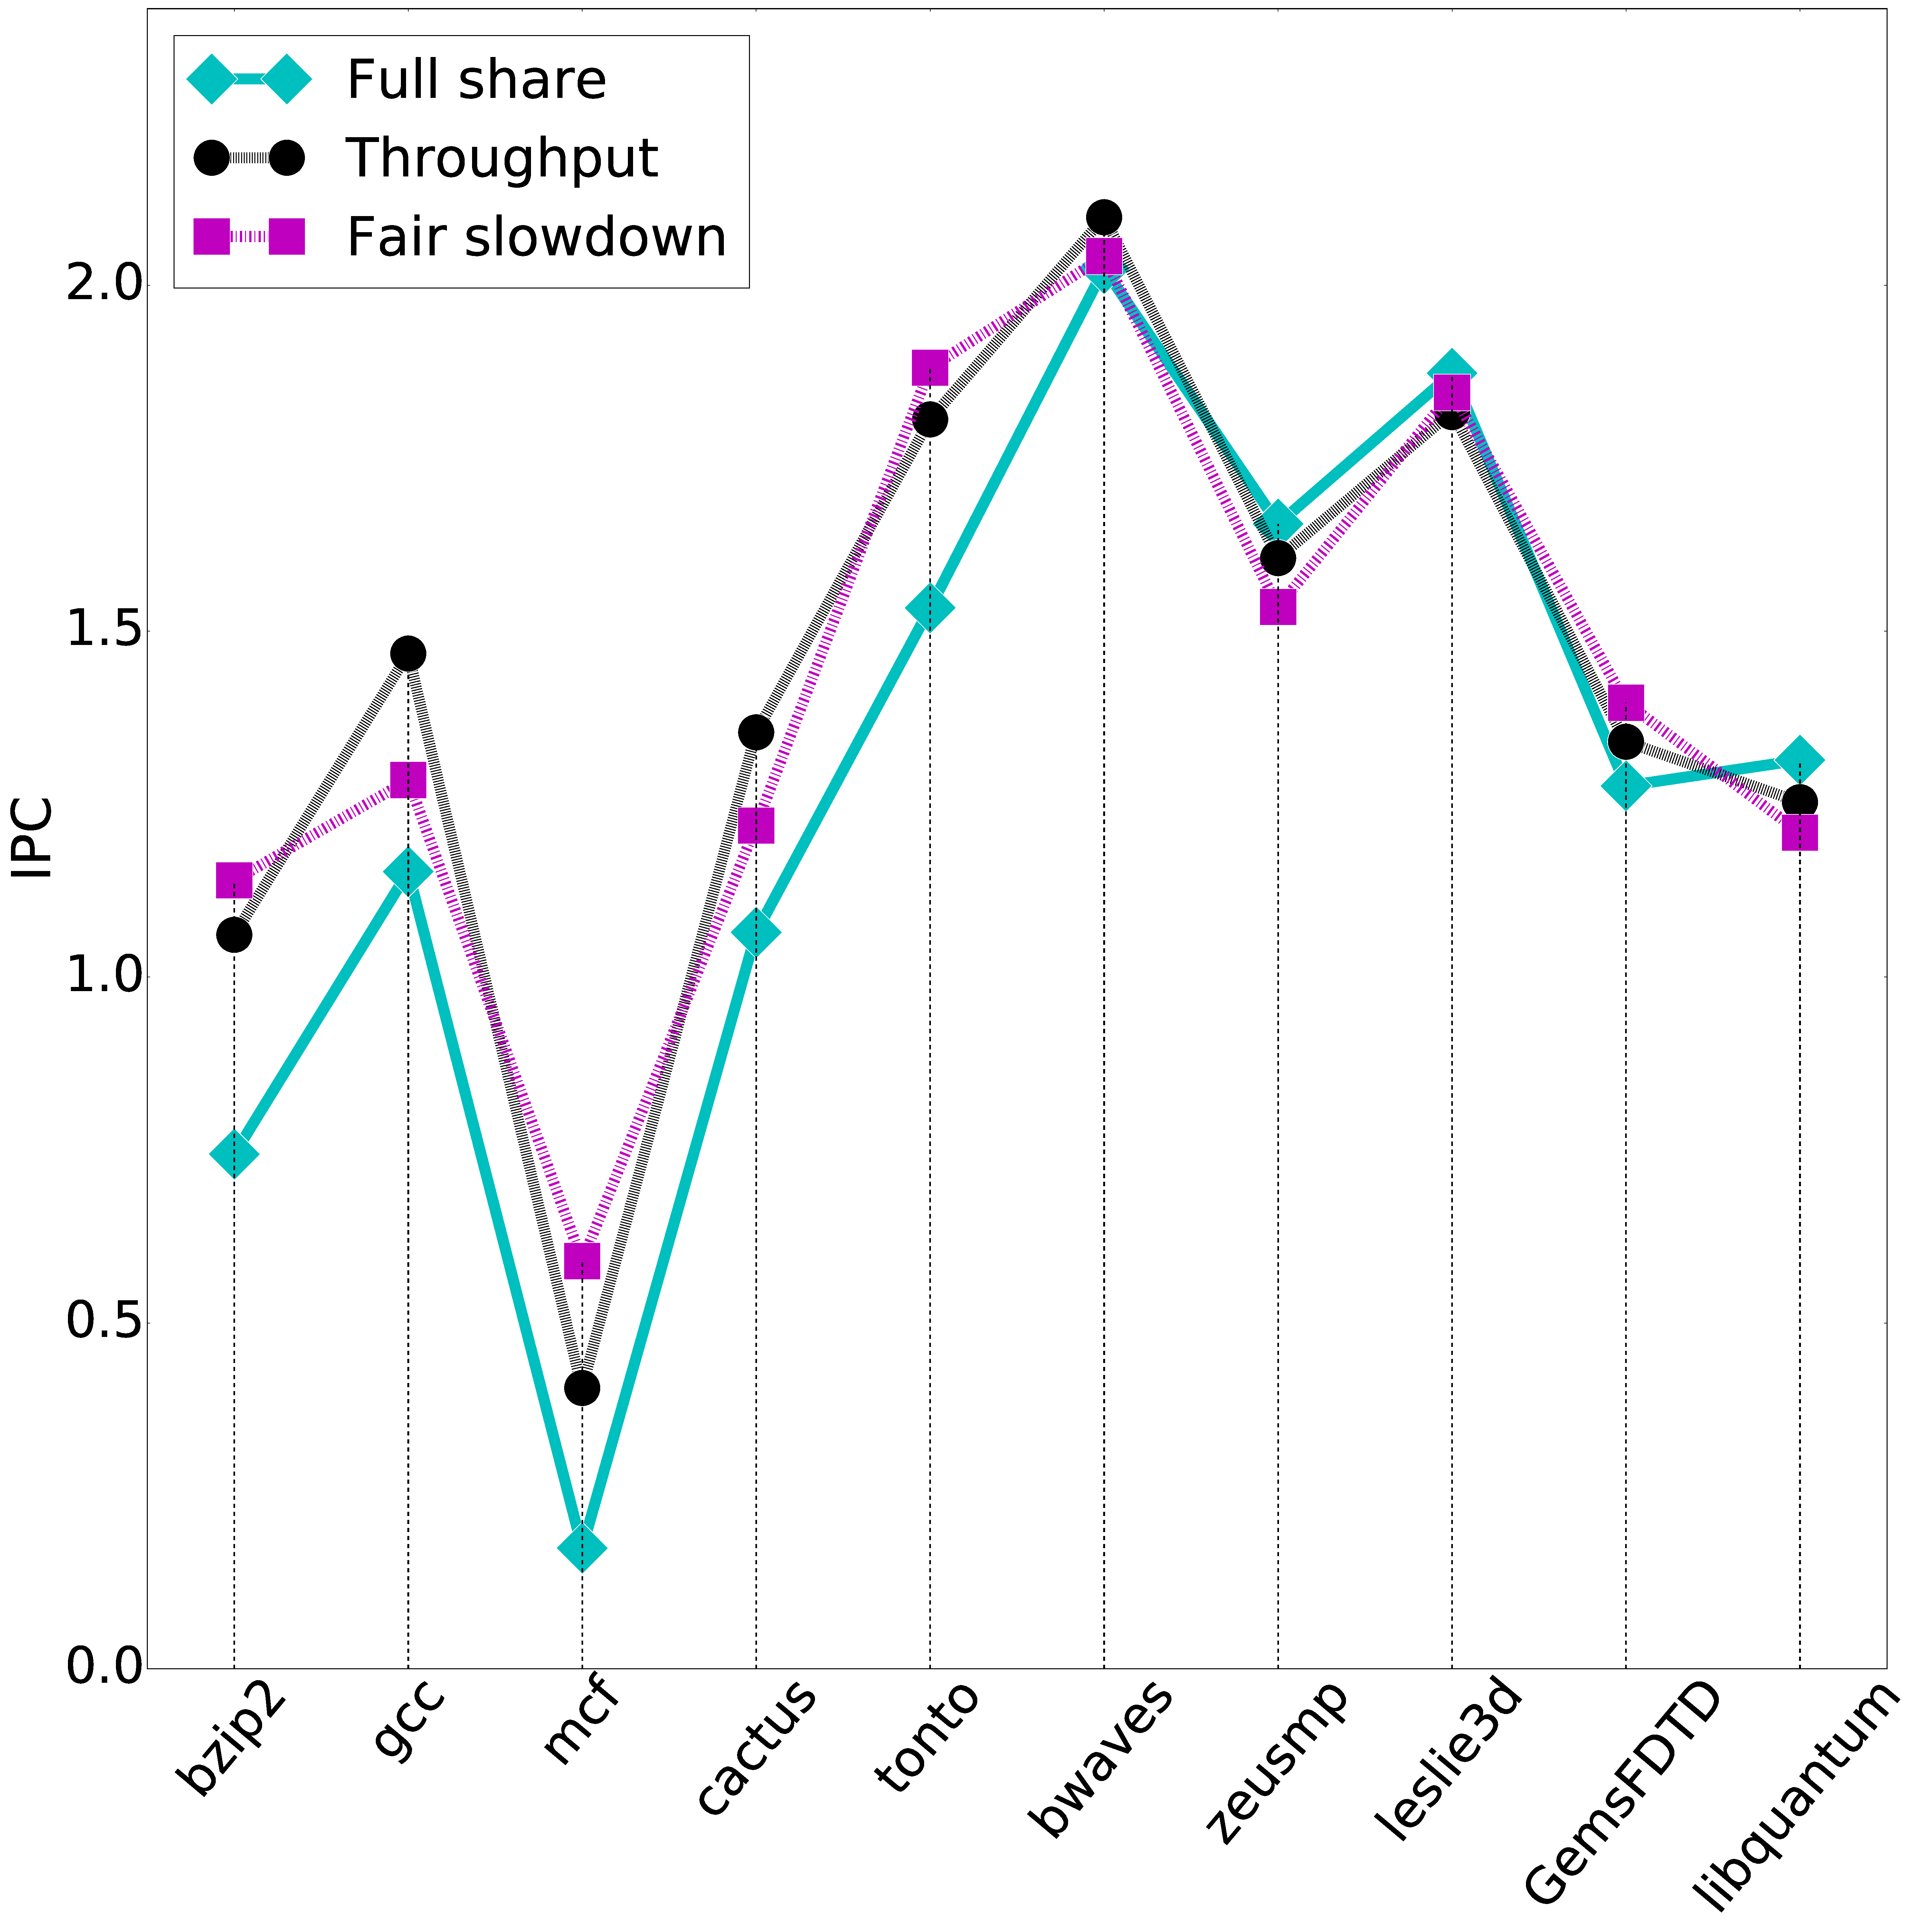
\includegraphics[width=0.8\columnwidth]{figures/case_ipc.pdf}
\caption{在自由竞争以及CAPS生成的Throughput和Fair slowdown方案下每个程序的IPC}
\label{fig:case_ipc}
\end{figure} 

虽然Throughput优化方案和Fair slowdown优化方案都会遵从多分配给A类程序、少分配给B类程序这一基本优化思路,但两种方案还是有一些不同之处。针对Throughput的吞吐量最大化方案会更加注重本身IPC就比较高的程序,因为提供同样大小的缓存给这类程序,往往在IPC数值的收益上会更大,而对于本身IPC较小的程序就会不太友好,因为从系统IPC的角度来看,给这类程序大量缓存空间并不会显著提高IPC的绝对数值。在另一方面,Fair slowdown策略关注的是IPC的变化率而不是绝对数值,因为slowdown就是通过IPC的变化比例来计算的,所以它对待高IPC和低IPC的程序会一视同仁。在这个D10的工作负载中,465.bzip2是一个高IPC程序,在单独运行的时候,它的IPC达到了1.70,而429.mcf是一个低IPC程序,它单独执行时的IPC只有0.58。在Throughput方案中,高IPC程序465.bzip相比于429.mcf得到了更大的缓存分配,因为这能大幅提升系统总体的IPC。而在Fair slowdown策略下,429.mcf的缓存分配反而比465.bzip更多,因为这能更好地缓解系统总体的slowdown。如图\ref{fig:case_ipc}所示,Throughput指标在Througput方案下是14.87,在Fair slowdown方案下是13.95;而Fair slowdown指在Throughput方案下是1.26,而在Fair slowdown方案下是1.21。与预期的一样,这两种方案都在各自锚定的指标上胜出了对方。
	% 结论。
	% Copyright (c) 2014,2016 Casper Ti. Vector
% Public domain.

\chapter{总结} \label{chap:conclusion}

随着多核处理器技术的普及,越来越多的处理器核被集成到单个处理芯片上。虽然这大大提高了处理器并发执行任务的能力,但存储访问的瓶颈问题却日益突出。并发执行的线程由于竞争使用底层共享缓存资源,从而造成严重的性能下降。因此,如何发现、控制和缓解对高速缓存等共享资源的竞争,提高并发系统的性能与隔离性,是多核环境中一个亟需探索的重要课题。

在本文中,我们提出了一个基于部分共享的高速缓存分配优化框架CAPS。这是一个纯软件的多目标优化框架,相比于以往的优化框架,它的主要优势有以下几点:

\begin{itemize}
    \item 可以在较细粒度层面实现对缓存占用的控制和管理
    \item 具有策略灵活性,可以支持多种优化目标
    \item 具有良好的可扩展性,在核数较多的情况下也同样适用
    \item 可以在真实机器上运行
\end{itemize}

CAPS依赖于英特尔最新发布的高速缓存分配技术(CAT),该技术是首次在商用处理器上实现的缓存分配技术。但是CAT本身是一种粗粒度的路分配技术(Way Partitioning),在核数/线程数较多时,效果会大打折扣。而CAPS通过分配之间的部分重叠,突破了CAT技术本身的这种限制,实现了细粒度的缓存分配。

CAPS的核心主要包含预测模型和分配算法两个部分。预测模型对于任意一个CAT分配方案下的多核工作负载可以预测出每个程序的失效率和IPC。分配算法是一个基于模拟退火的优化算法,对于一个指定的优化目标,可以产生一个优化分配方案,这个方案可能是部分重叠的,并可以直接被CAT技术所应用。

同时CAPS可以支持多种优化目标,并且对于不同的目标,只需要改动目标估值函数,而不需要对策略算法做很大的改动。我们在真实环境中对CAPS进行了大量的实验,结果显示CAPS生成的部分重叠方案在五种优化指标上都能起到良好的优化效果。

目前CAPS只支持静态优化,需要离线对程序进行采样分析。在未来,我们希望把CAPS拓展到在线场景中,可以根据当前执行的程序特征,动态地调整优化方案。


	% 正文中的附录部分。
	\appendix
	% 排版参考文献列表。bibintoc 选项使“参考文献”出现在目录中;
	% 如果同时要使参考文献列表参与章节编号,可将“bibintoc”改为“bibnumbered”。
	\printbibliography[heading = bibintoc]
	% 各附录。
	% % Copyright (c) 2014,2016 Casper Ti. Vector
% Public domain.

\chapter{附件}
\pkuthssffaq % 中文测试文字。

% vim:ts=4:sw=4


	% 以下为正文之后的部分,默认不进行章节编号。
	\backmatter
	% 致谢。
	% Copyright (c) 2014,2016 Casper Ti. Vector
% Public domain.

\chapter{致谢}
\pkuthssffaq % 中文测试文字。

% vim:ts=4:sw=4

	% 原创性声明和使用授权说明。
	% Copyright (c) 2008-2009 solvethis
% Copyright (c) 2010-2017 Casper Ti. Vector
% All rights reserved.
%
% Redistribution and use in source and binary forms, with or without
% modification, are permitted provided that the following conditions are
% met:
%
% * Redistributions of source code must retain the above copyright notice,
%   this list of conditions and the following disclaimer.
% * Redistributions in binary form must reproduce the above copyright
%   notice, this list of conditions and the following disclaimer in the
%   documentation and/or other materials provided with the distribution.
% * Neither the name of Peking University nor the names of its contributors
%   may be used to endorse or promote products derived from this software
%   without specific prior written permission.
%
% THIS SOFTWARE IS PROVIDED BY THE COPYRIGHT HOLDERS AND CONTRIBUTORS "AS
% IS" AND ANY EXPRESS OR IMPLIED WARRANTIES, INCLUDING, BUT NOT LIMITED TO,
% THE IMPLIED WARRANTIES OF MERCHANTABILITY AND FITNESS FOR A PARTICULAR
% PURPOSE ARE DISCLAIMED. IN NO EVENT SHALL THE COPYRIGHT HOLDER OR
% CONTRIBUTORS BE LIABLE FOR ANY DIRECT, INDIRECT, INCIDENTAL, SPECIAL,
% EXEMPLARY, OR CONSEQUENTIAL DAMAGES (INCLUDING, BUT NOT LIMITED TO,
% PROCUREMENT OF SUBSTITUTE GOODS OR SERVICES; LOSS OF USE, DATA, OR
% PROFITS; OR BUSINESS INTERRUPTION) HOWEVER CAUSED AND ON ANY THEORY OF
% LIABILITY, WHETHER IN CONTRACT, STRICT LIABILITY, OR TORT (INCLUDING
% NEGLIGENCE OR OTHERWISE) ARISING IN ANY WAY OUT OF THE USE OF THIS
% SOFTWARE, EVEN IF ADVISED OF THE POSSIBILITY OF SUCH DAMAGE.

{
	\ctexset{section = {
		format+ = {\centering}, beforeskip = {40bp}, afterskip = {15bp}
	}}

	% 学校书面要求本页面不要页码,但在给出的 Word 模版中又有页码且编入了目录。
	% 此处以 Word 模版为实际标准进行设定。
	\specialchap{北京大学学位论文原创性声明和使用授权说明}
	\mbox{}\vspace*{-3em}
	\section*{原创性声明}

	本人郑重声明:
	所呈交的学位论文,是本人在导师的指导下,独立进行研究工作所取得的成果。
	除文中已经注明引用的内容外,
	本论文不含任何其他个人或集体已经发表或撰写过的作品或成果。
	对本文的研究做出重要贡献的个人和集体,均已在文中以明确方式标明。
	本声明的法律结果由本人承担。
	\vskip 1em
	\rightline{%
		论文作者签名:\hspace{5em}%
		日期:\hspace{2em}年\hspace{2em}月\hspace{2em}日%
	}

	\section*{%
		学位论文使用授权说明\\[-0.33em]
		\textmd{\zihao{5}(必须装订在提交学校图书馆的印刷本)}%
	}

	本人完全了解北京大学关于收集、保存、使用学位论文的规定,即:
	\begin{itemize}
		\item 按照学校要求提交学位论文的印刷本和电子版本;
		\item 学校有权保存学位论文的印刷本和电子版,
			并提供目录检索与阅览服务,在校园网上提供服务;
		\item 学校可以采用影印、缩印、数字化或其它复制手段保存论文;
		\item 因某种特殊原因需要延迟发布学位论文电子版,
			授权学校在 $\Box$\nobreakspace{}一年 /
			$\Box$\nobreakspace{}两年 /
			$\Box$\nobreakspace{}三年以后在校园网上全文发布。
	\end{itemize}
	\centerline{(保密论文在解密后遵守此规定)}
	\vskip 1em
	\rightline{%
		论文作者签名:\hspace{5em}导师签名:\hspace{5em}%
		日期:\hspace{2em}年\hspace{2em}月\hspace{2em}日%
	}

	% 若需排版二维码,请将二维码图片重命名为“barcode”,
	% 转为合适的图片格式,并放在当前目录下,然后去掉下面 2 行的注释。
	%\vfill\noindent
	%\includegraphics[height = 5em]{barcode}
}

% vim:ts=4:sw=4

\end{document}

% vim:ts=4:sw=4
